% First-pass transcriptions of cote 147 by GPT-6 Astra (ChatGPT Pro mode), 10-11 Nov 2026; not yet second-passed.

% ===== MPL_147_003-047 (first pass) =====
\scanpage{3}
\uline{Structure à l'$\infty$ des $M_{g,\nu}$}

\begin{tabular}{r p{0.79\linewidth} r}
1. & Courbes standard & 1 \\
2. & Graphe associé à une courbe standard\newline \unsure{Maquettes} & 3 \\
3. & Courbes stables, et MD-graphes & 6 \\
4. & Le théorème de Mumford-Deligne & 10 \\
5. & Spécialisation de MD-graphes & 15 \\
6. & Morphismes de générisation de graphes et de \unsure{maquettes} & $16'$ \\
7. & Étude des $\widehat M_{g,\unsure{\nu}}$ de dim $\leq 2$ : a) détermination des graphes correspondants & 25 \\
8. & Structure \unsure{de|des} spécialisation des strates en dim. modulaire ambiante $\leq \unsure{4}$ & $29'$ \\
9. & Structure groupoïdale \deleted{des} multiplicités modulaires de Teichmüller compactes (la MDT-structure) : Construction, morphismes de générisation & 37 \\
10. & Structure MDT analytique : \unsure{action} des morphismes de normalisation entre MD-graphes & 45 \\
11. & Digression : déploiement d'un diviseur à croisements normaux. Structure à l'infini des groupoïdes fondamentaux & 52 \\
12. & Digression (suite) : types canoniques associés à une stratification par croisements normaux, et leur dévissage en ``types élémentaires'' & 74 \\
13. & Digression sur stratifications \inserted{``locales''} générales & 86
\end{tabular}
\mspage{2}
\scanpage{4}
Structure à l'infini des $M_{g,\nu}$

1. \uline{Courbes \unsure{standard|standart}}.

Soit $k$ un corps alg. clos. Une ``courbe \unsure{standard|standart}'' sur $k$ est un\deleted{e \unsure{courbe}} schéma $X$ sur $k$ satisfaisant les conditions suivantes :

a) $X$ quasi-projectif, \inserted{toute composante irréd. est} de dim $1$

b) Tout point de $X$ est soit lisse, soit un ``point quadratique'' (``ordinaire'') -- i.e. isom. (loc. ét) à la courbe $\operatorname{Spec}(k[X,Y]/XY)$ au point $0$.

Il est connu qu'on peut donner une unique ``complétion'' $\widehat X$ de $X$, telle que \inserted{$\widehat X$ soit un schéma propre, \unsure{que}} $X$ s'identifie à un ouvert dense de $\widehat X$, et que $\widehat X$ soit lisse en les pts de $\widehat X\setminus X=I$. Alors $\widehat X$ est une courbe projective, $I$ est \deleted{\unsure{contenu}} une partie finie de $\widehat X(k)$ contenue dans l'ens. ouvert des pts de lissité de $\widehat X$. L'ens. $A$ des pts singuliers de $X$ s'identifie à l'ens. analogue pour $\widehat X$
\[
(1)\qquad
\left\{\begin{aligned}
I&=\widehat X\setminus X\subset\widehat X^{\mathrm{lisse}}(k)
&&\text{``pts à l'infini'' de }X\\
A&=X\setminus X^{\mathrm{lisse}}=\widehat X\setminus\widehat X^{\mathrm{lisse}}\subset X(k)
&&\text{(pts singuliers de }X\text{)}
\end{aligned}\right.
\]
La donnée de $X$ équivaut à celle de
\mspage{3}
\scanpage{5}
$(\widehat X,I)$, où $\widehat X$ est un schéma projectif, dont \unsure{tte} composante irréductible est de dim $1$, et dont l'ensemble singulier est formé de pts quadratiques ordinaires -- et $I$ est un sous-schéma fini étale de $\widehat X^{\mathrm{lisse}}$, ou ce qui revient au $=$, une partie finie de $\widehat X^{\mathrm{lisse}}(k)$.

Soit $\widetilde{\widehat X}=\widehat{\widetilde X}$ le normalisé de $\widehat X$, \deleted{alors}
\[
\widetilde I=\widehat{\widetilde X}\setminus\widetilde X
=\text{Image inverse de }I\text{ par }\widetilde{\widehat X}\to\widehat X
\]
l'ens. des \deleted{ses} ``points à l'infini'' de $\widetilde X$, on a
\[
(2)\qquad\widetilde I\xrightarrow{\sim}I
\]
et nous identifions généralement $\widetilde I$ et $I$, et plus généralement \deleted{$\unsure{\widehat X^{\mathrm{lisse}}}$ \unsure{à}} les pts de $\widehat X^{\mathrm{lisse}}$ aux pts correspondants de $\widetilde{\widehat X}$. Soit $\widetilde A$ l'image inverse de $A$ dans $\widetilde X$ (ou dans $\widehat{\widetilde X}$), alors
\[
(3)\qquad\widetilde A\longrightarrow A
\]
est une application de degré $2$, d'où une involution sans pts \unsure{fixe|fixes} $\sigma_{\widetilde A}$ dans $\widetilde A$.

Ainsi, à la courbe \unsure{standard|standart} $X$ nous avons associé \unsure{le système|les systèmes} de données
\mspage{4}
\scanpage{6}
\mspage{2}
suivant :
\[
(4)\quad\left\{\begin{aligned}
&\text{a) Une courbe projective et lisse }Y(=\widehat{\widetilde X})\deleted{\unsure{sur }k}\\
&\text{b) Deux parties }\inserted{\text{finies}}\text{ disjointes }\widetilde A\text{ et }I\text{ de }Y(k)\\
&\text{(ou encore, deux sous-schémas finis étales}\\
&\text{disjoints }\widetilde A_k\text{ et }I_k\text{ de }Y\text{)}\\
&\text{c) Une involution sans point fixe }\sigma_{\widetilde A}\text{ de}\\
&\widetilde A\text{ (qui est donc de cardinal pair).}
\end{aligned}\right.
\]
Inversement, partant de données a) b) c), on construit une courbe \unsure{standard|standart} $X$ en passant au quotient dans $Y\setminus I_k\supset\widetilde A_k$ par l'involution $\sigma$ -- i.e. $X$ est universel \inserted{(dans (Sch))} pour la donnée $p$ :
\diagram{\begin{tikzcd}
Y\setminus I_k\arrow[r,"p"] & X\\
\bigl(\,\widetilde A_k\arrow[u,"i"]\arrow[ur,dashed] & \bigr)
\end{tikzcd}}
, soumise à $(pi)\sigma=pi$.

Ainsi la catégorie des courbes \unsure{standard|standart} sur $k$ \inserted{(pour les iso)} apparaît comme équivalente à celle des systèmes a) b) c) ci-dessus. (pour les iso)\ldots

\uline{NB} On récupère $\widehat X$ comme quotient de $Y$ par $\sigma$.
\mspage{5}
\scanpage{7}
\uline{Généralisation sur une base quelconque.}

Une \uline{courbe \unsure{standard|standart}} sur $S$ (multiplicité schématique, disons) sera \unsure{définie|défini} constructivement en termes d'un système a) b) c) \inserted{comme} ci-dessus, i.e.
\[
(5)\quad\left\{\begin{aligned}
&\text{a) }Y,\text{ schéma propre et lisse }\inserted{\text{sur }S}\text{ partout de}\\
&\text{dim relative }1;\\
&\text{b) }\widetilde A\text{ et }I,\text{ deux sous-schém. de }Y,\\
&\text{finis étales sur }S,\quad\deleted{\unsure{\text{avec}}}\ \widetilde A\cap I=\varnothing;\\
&\text{c) }\sigma_{\widetilde A}\text{ une involution de }\widetilde A,\text{ opérant}\\
&\text{librement.}
\end{aligned}\right.
\]
On construit alors $\widehat X=\unsure{Y}/\sigma$, contenant $A\simeq\widetilde A/\sigma$ et $I$ comme sous-schémas \inserted{fermés} finis étales sur $S$, et on définit $X=\widehat X\setminus I$. On peut montrer que le foncteur
\[
(6)\qquad(Y,\widetilde A,\inserted{I,}\sigma_{\widetilde A})\longmapsto X
\]
\margin{\uline{NB} NB ce foncteur est compatible aux images inverses\ldots}
des systèmes (5) (pour les iso) vers les schémas relatifs, \inserted{(pour les iso)} est \uline{pleinement fidèle}.
\margin{faux tel quel !}
\mspage{6}
\scanpage{8}
\mspage{3}
\margin{Le foncteur est pl. fid. au mieux sur une base $S$ réduite -- faux p. ex. sur les \unsure{nbs} duaux d'un corps (si $I\neq\varnothing$). Pour avoir un foncteur pl fidèle, il faut \unsure{se placer} dans le contexte \uline{propre}, i.e. \unsure{remplacer} $X$ par $(\widehat X,I)$ (de sorte que $X=\widehat X-I$).}
J'appelle ``courbe \inserted{relative} \unsure{standard|standart}'' sur $S$, tout élément de l'image essentielle. Le système $(Y,\widetilde A,I,\sigma)$ qui lui donne naissance s'appellera le ``complété normalisé'' \inserted{(relatif)} (par abus de \deleted{système définissant} langage, puisque c'est non seulement le schéma relatif $Y$, mais $Y$ avec la structure supplémentaire $\widetilde A,I,\sigma_{\widetilde A}\ldots$).

2. \uline{Graphe associé à une courbe \unsure{standard|standart}.}

Revenons au cas d'un corps de base $k$ alg. clos, pour commencer. Soit $\unsure{X}$ une courbe \unsure{standard|standart}, d'où $Y,\deleted{\unsure{\widetilde A},}I,\widetilde A,\sigma_{\widetilde A}$.

Posons
\[
(7)\qquad S=\pi_0(Y)\simeq\text{ens. des comp. irréd. de }X
\]
On a alors le diagramme d'applications canoniques entre ensembles finis
\[
(8)\qquad
\diagram{\begin{tikzcd}
& I\arrow[d,"p"]\\
\widetilde A\arrow[r,"\unsure{o|\sigma}"]\arrow[d,"q"'] & S\\
A=\widetilde A/\sigma &
\end{tikzcd}}
\]
\mspage{7}
\scanpage{9}
où $q$ est de degré $2$ et définit l'involution $\sigma_{\widetilde A}$. Les applications $o$ et $p$ sont induites par les inclusions $\widetilde A\hookrightarrow Y$, $I\hookrightarrow Y$ en passant aux $\pi_0$.

Le système
\diagram{\begin{tikzcd}
\bigl(\widetilde A\arrow[r,"o"] & S,\sigma_{\widetilde A}\bigr)
\end{tikzcd}}
ou
\diagram{\begin{tikzcd}
\bigl(\widetilde A\arrow[r,"o"]\arrow[d,"\text{deg 2}"'] & S\bigr)\\
A &
\end{tikzcd}}
, peut être considéré comme définissant un \uline{graphe}, dont $S$ est l'ens. des sommets, et $\widetilde A$ l'ens. des \uline{arcs} (ou arêtes orientées) l'application $o$ étant l'application ``origine d'un arc''. Ce graphe ne dépend que de $\widehat X$, pas de $X$ i.e. du choix de $I\subset\widehat X(k)$. C'est pour tenir compte de ce choix que l'on considère, en plus de la structure de graphe, la donnée supplémentaire
\[
(9)\qquad I\longrightarrow S
\]
\mspage{8}
\scanpage{10}
\mspage{4}
Le graphe indique comment les composantes irréductibles de $X$ (\unsure{figurées|figurés} par les sommets) se rencontrent deux à deux -- les pts d'intersection, i.e. les pts singuliers (\inserted{``doubles'', \unsure{sc.}}quadratiques) de $X$, correspondent aux arêtes. Si une composante irréductible $X_\alpha$ de $X$ correspond au sommet $\alpha$ du graphe, alors les boucles fermées en $\alpha$ correspondent biunivoquement aux pts doubles de $X_\alpha$ -- donc dire que les $X_\alpha$ sont lisses signifie que le graphe $G_X$ n'a pas de boucles fermées, i.e. que pour tt arc, l'origine est $\neq$ de l'extrémité.

Il est clair que tout graphe fini peut être obtenu \inserted{(à iso près)} \deleted{à l'aide} par une $\widehat X$ convenable -- et $\unsure{=|\overline m}$ avec des \unsure{compo-}
\mspage{9}
\scanpage{11}
santes $X_\alpha$ de genre \inserted{$g_\alpha$} donné (i.e. des $\widetilde X_\alpha$ de genre $g_\alpha\ldots$). De plus, quand on se donne \deleted{\unsure{des}} $I\to S$ ($I$ ens fini), cela peut être réalisé par un $I\subset\widehat X^{\mathrm{lisse}}$, i.e. par une courbe \unsure{standard|standart} $S$.

La \uline{maquette} d'une courbe \unsure{standard|standart} $X$ consiste, par définition, en les données suivantes
\[
(10)\quad\left\{\begin{aligned}
&\text{a) le graphe }G_X=\biggl(
\underset{\inserted{\substack{\Vert\\\pi_0(\widetilde X)\\\Vert\\\pi_0(\widehat{\widetilde X})}}}{S},
\underset{\inserted{\substack{\Vert\\\unsure{\operatorname{Sing}(X)}}}}{\widetilde A},
\underset{\deleted{\unsure{\widehat X}}}{\sigma_{\widetilde A}}
\biggr)\\
&\text{b) L'}\deleted{\text{application}}\inserted{\text{ensemble}}\ I=\widehat X\setminus X,\text{ et l'application}\\
&\qquad I\longrightarrow S\\
&\text{c) L'application}\\
&\qquad S\xrightarrow{\uline{g}}\mathbb N\\
&\qquad\alpha\longmapsto\text{genre de }Y_\alpha=\widehat{\widetilde X}_\alpha
\end{aligned}\right.
\]
Une structure formée d'un graphe fini $G$\inserted{$=(S,\widetilde A,\sigma_{\widetilde A})$}, d'un ensemble fini $I$ \deleted{\unsure{de}} au dessus de l'ens. des sommets $S$ de $G$, et d'une application \inserted{``genre''} : $S\xrightarrow{\uline{g}}\mathbb N$, sera
\mspage{10}
\scanpage{12}
\mspage{5}
appelé ici une ``maquette''.

\uline{Proposition} \inserted{Considérons la maquette d'une courbe \unsure{standard|standart} $X$.}
a) Soient $\alpha,\beta\in S$, alors $\alpha,\beta$ appartiennent à la $=$ composante conn. du graphe $G$, ssi. $X_\alpha$ et $X_\beta$ appartiennent à la $=$ comp. conn. de $X$. Donc \deleted{\unsure{l'on}} on a une bij. can.
\[
(11)\qquad\pi_0(G_X)\simeq\pi_0(X),
\]
en particulier $X$ est connexe ssi $G_X$ est connexe.

b) Supposons $X$ connexe i.e. $\widehat X$ connexe, i.e. $H^0(\widehat X,\underline O_{\widehat X})\unsure{\xleftarrow{\sim}|\simeq}k$ i.e dim $H^0(\widehat X,\underline O_{\widehat X})=1$.

Posons \deleted{$g(X)=\dim H^1(X,\underline O_X),\quad\chi(X)=\chi$}
\[
(12)\quad\left\{\begin{aligned}
g(\widehat X)&=\dim H^1(\widehat X,\underline O_{\widehat X})\\
\chi_{\mathrm{coh}}(\widehat X)&=\chi(X\deleted{\unsure{g}},\underline O_X)=1-g(X)
\end{aligned}\right.,
\]
on a alors
\[
(13)\quad\chi_{\mathrm{coh}}(\widehat X)
=\deleted{\unsure{\sum_{\alpha\in S}\chi_{\mathrm{coh}}(\widehat{\widetilde X}_\alpha)}}
\inserted{\chi(\widetilde{\widehat X})-\underbrace{\operatorname{card}A}_{\mu}}
=\sum_{\alpha\in S}(1-g_\alpha)-\mu
\]
i.e.
\[
(14)\quad\left\{\begin{aligned}
g(\widehat X)&=\sum g_\alpha+(-\operatorname{card}S+\underbrace{\operatorname{card}A}_{\mu}+1)\\
&=\sum g_\alpha+h_1
\end{aligned}\right.,
\]
\mspage{11}
\scanpage{13}
où \deleted{$\unsure{h_1}$ \unsure{est le}}
\[
(15)\qquad h_1=\operatorname{rg}_{\mathbb Z}H_1(G_X,\mathbb Z).
\]
\uline{Démonstration} \unsure{Standard|Standart} (!) -- la formule (13) résulte d'une suite exacte \inserted{\unsure{standard|standart}} de cohomologie reliant $\underline O_{\widehat X}$, $\underline O_{\widetilde{\widehat X}}$ et les singularités de $\widehat X$, d'ailleurs la formule d'EP pour le graphe $G_X$ nous donne
\[
\chi(G_X)=\underbrace{h_0}_{1}\deleted{\unsure{(G_X)}}-h_1=\operatorname{card}S-\operatorname{card}A
\]
i.e.
\[
1-\operatorname{card}S+\operatorname{card}A=h_1\qquad\text{O.K.}
\]
\uline{Corollaire} Le nb $g(\widehat X)$ ne dépend que de la maquette de $X$, par la formule (14)
\[
g(\widehat X)=\underbrace{\sum_{\alpha\in S}g(\alpha)+h_1}_{\overset{\mathrm{dfn}}{=}\ \text{genre de }G}
\]
-- on l'appelle le \uline{genre} de la maquette.

On appelle \uline{type} de la maquette le couple $(\unsure{\bar g|g},\nu)$, où $g$ est son genre et $\nu=\operatorname{card}I$ est le \uline{poids marqué}. On appelle \uline{poids marqué} d'un sommet l'entier naturel
\mspage{12}
\scanpage{14}
\mspage{6}
\margin{c'est le nb de pts à l'infini de la composante $X_\alpha$}
$\operatorname{card}I_\alpha$ (où $I_\alpha$ est la fibre de $I$ en $\alpha\in S$)
\[
(16)\qquad\nu_\alpha=\operatorname{card}I_\alpha,
\]
et on appelle \uline{poids total} d'un sommet l'entier
\[
(17)\qquad\widehat\nu_\alpha=\nu_\alpha+
\underset{\substack{\Vert\ \mathrm{déf}\\
\text{ordre du sommet }\alpha,\\
\text{i.e. }\operatorname{card}\widetilde A_\alpha,\text{ où }\widetilde A_\alpha\text{ est la fibre}\\
\text{de }\widetilde A\text{ au dessus de }\alpha,\text{ i.e. le}\\
\text{nb d'arcs sortant de }\alpha}}{\omega_\alpha}
\]
c'est donc le nb de ``pts marqués'' (provenant de pts doubles \unsure{et} de pts à l'infini de $X$) sur la composante $Y_\alpha$ de $Y=\widetilde{\widehat X}$.

3. \uline{Courbes ``stables''.} \uline{et} \uline{MD-graphes.}

Une courbe \unsure{standard|standart} \inserted{(sur $k$ alg. clos)} est ``stable'', si elle satisfait à l'une des conditions équivalentes suivantes

a) $\operatorname{Aut}X$ est fini

b) Pour tout $\alpha$, $(Y_\alpha,I_\alpha\cup\widetilde A_\alpha)$ est anabélien
\[
\text{i.e.}\quad 2g_\alpha+\widehat\nu_\alpha\geq3\qquad
\text{i.e.}\quad 2g_\alpha-2+\widehat\nu_\alpha\geq1,\quad\text{i.e.}
\]
\mspage{13}
\scanpage{15}
1°) Si $g_\alpha=1$, on a $\widehat\nu_\alpha\geq1$

2°) Si $g_\alpha=0$ on a $\widehat\nu_\alpha\geq3$

c) Tout champ de vecteurs sur $Y$ nul sur $\deleted{\unsure{\widetilde A}}I\cup\widetilde A$ est nul.

d) $\underline{\operatorname{Aut}}_{(Y,\widetilde A_k,I)}$ est un schéma en groupes fini étale sur $k$.

On voit que cette condition (sous la forme b)) ne dépend que de la \uline{maquette} de la courbe. On dit que $X$ est une \uline{MD-courbe} (MD, initiales de ``Mumford-Deligne'' -- ou de ``modulaire'') si elle est stable, et \inserted{0-}connexe \inserted{(i.e. connexe non vide)}.

Les maquettes de telles courbes sont les maquettes $0$-connexes \inserted{et} stables (i.e. dont les sommets de genre $1$ sont de poids total $\geq1$, et les sommets de genre $0$ sont de poids total $\geq3$), on les appellera les MD-graphes.

\uline{NB} Une maquette est un MD-graphe ssi

a) elle est $0$-connexe (i.e. le graphe $G$ est conn. $\neq\varnothing$)

b) elle n'est pas réduite à un seul sommet de genre $1$, de poids total $0$ (pas d'arête, pas de points marqués)

c) les sommets de genre $0$ sont de poids total $\geq3$.
\mspage{14}
\scanpage{16}
\mspage{7}
\uline{Proposition} Si $(G=(S,\widetilde A,\sigma),I,g:S\to\mathbb N)$ est un MD-graphe, son type $(g,\nu)$ est anabélien, i.e. $2g+\nu\geq3$.

Si on avait $g=1$, $\nu=0$, alors la relation
\[
g=1=\sum g_\alpha+h_1
\]
montre que ou bien tous les $g_\alpha$ sont nuls, et $h_1=1\deleted{\unsure{+1}}$, ou bien tous les $g_\alpha$ sauf un \inserted{$g_{\alpha_0}$} sont nuls, et $g_{\alpha_0}=1$, $h_1=0$ \inserted{(i.e. $G$ est un arbre)}. \inserted{Dans le premier cas,} La relation $s_0-s_1=h_0-h_1=1-1=0$ montre qu'il y a autant de sommets que d'arêtes, dans le deuxième, $s_0-s_1=1-0=1$ il y a un sommet de plus que d'arêtes.

Mais la relation $\nu=0$ implique que les sommets de genre $0$ sont d'ordre $\geq3$. \inserted{$G$ n'est pas réduit à un sommet, puisqu'il est stable de type $(1,0)$.} Mais un \deleted{graphe top. compact \unsure{ou}} \inserted{arbre qui \unsure{n'est réduit} à un seul sommet} a au moins deux bouts, dont l'un au moins sera de genre $0$, ce qui élimine le cas 2°. Donc tous les sommets sont de genre nuls \inserted{(donc aucun sommet n'est un bout)} et $h_1=\unsure{1}$. Mais \deleted{\unsure{comme}} un graphe topologique $0$-connexe avec $h_1=1$ qui n'a pas de \inserted{pt.} bord topologique est homéomorphe au cercle, donc s'il est réalisé par un graphe combinatoire, tous les sommets de celui-ci sont d'ordre $2$, ce qui contredit qu'ils soient d'ordre trois.
\mspage{15}
\scanpage{17}
Éliminons de $=$ le cas $g=0$, $\nu\leq2$. Ici $g=0=\sum g_\alpha+h_1$ implique que les $g_\alpha$ et $h_1$ sont nuls : tous les sommets sont de genre $0$, le graphe est un arbre. Il ne peut être réduit à un seul sommet, donc il a au moins deux bouts, dont les \unsure{poids} marqués doivent être $\geq2$, donc \deleted{\unsure{le}} on a $\nu\geq2+2=4$, absurde.

Soit $G$ une \deleted{\inserted{MD-}graphe}\inserted{maquette}. On dit qu'une \deleted{\inserted{MD-}} courbe \deleted{\unsure{standard|standart}}\inserted{\unsure{standard|standart}} $C$ sur un corps alg. clos est de \uline{type $G$}, si sa maquette est iso à $G$, on dit qu'elle est \inserted{$G$-}\uline{épinglée} si on se donne un iso entre sa maquette et $G$ (c'est donc une structure suppl. sur $\unsure{C|X}$, appelée $G$-épinglage).

Soit $(\widehat X,I)$ une courbe \unsure{standard|standart} sur une base $S$ quelconque, on dit qu'elle est de type $G$ si ses fibres géom. sont de type $G$. Alors les \deleted{\unsure{``types'' des}}\inserted{maquettes} des
\mspage{16}
\scanpage{18}
\mspage{8}
fibres géom. de $(\widehat X,\underline I)$ forment les fibres d'un schéma en maquettes \inserted{(ou en MD-graphes)} sur $\unsure{\mathcal S|S}$
\[
(\deleted{\unsure{\underline G|\underline S}}\underline S,\underline{\widetilde A},\sigma_{\underline{\widetilde A}},\underline I,\ \underline{\widetilde A}\to\underline S,\ \underline I\to\underline S,\ \inserted{\underline S\xrightarrow{\underline g}\mathbb N_{\mathcal S}})
\]
(système de rev. finis étales \inserted{de $\mathcal S$} et de morphismes entre ceux-ci), loc. isomorphes à la maquette $G$ donnée. \deleted{\unsure{Le}} On appelle \inserted{$G$-}épinglage de $(\widehat X,\underline I)$ tout isomorphisme entre $G_{\mathcal S}$ et $\underline G(\widehat X,\underline I)$. Si \deleted{$\unsure{\Gamma}$}
\[
(18)\qquad\Gamma=\operatorname{Aut}G
\]
(groupe fini), les $G$-épinglages de $(\widehat X,\underline I)$ s'identifient aux sections d'un certain $\Gamma_{\mathcal S}$-torseur, \deleted{\unsure{qui est le|qui sera le}}\inserted{appelé} \uline{torseur des $G$-épinglages} de $(\widehat X,\underline I)$.

Considérons, sur une base $\mathcal S$ fixée, la catégorie \inserted{(pour les iso)} des courbes standard $G$-épinglées. Pour tt $\alpha\in S$ (ens. des sommets de la maquette) soit $\widehat I_\alpha=I_\alpha\amalg\widetilde A_\alpha$ l'ensemble (de cardinal $\widehat\nu_\alpha=\text{poids total de }\alpha$) somme
\mspage{17}
\scanpage{19}
des fibres $I_\alpha$ et $\widetilde A_\alpha$ de $I$ et $A$ au dessus de $\alpha$. La donnée d'une courbe \unsure{standard|standart} $G$ épinglée sur $\mathcal S$ équivaut à la donnée, \deleted{de} pour $\forall\ \alpha\in S$, d'une courbe relative (propre lisse \inserted{relt} $0$-connexe) $Y_\alpha$ sur $\mathcal S$, de genre relatif $g_\alpha$, \uline{et} d'un \inserted{$\mathcal S$-}mono. $(\widehat I_\alpha)_{\mathcal S}\hookrightarrow Y_\alpha$.

Désignons, \deleted{par $\mathcal M_{g_\alpha,\deleted{\nu_\alpha}\inserted{\widehat I_{\unsure{\alpha}}}}$} pour \deleted{\unsure{de}}\inserted{un} entier naturel $g\deleted{\unsure{\alpha}}$ et un ens. fini $I$ (de cardinal $\nu$) par
\figure{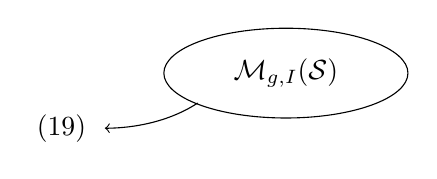
\begin{tikzpicture}[baseline=(m.base)]
\node (m) at (0,0) {$\mathcal M_{g,I}(\mathcal S)$};
\draw (0,0) ellipse (1.55 and .57);
\draw[->] (-1.12,-.38) .. controls (-1.55,-.66) and (-2.05,-.7) .. (-2.3,-.7);
\node at (-2.85,-.7) {$(19)$};
\end{tikzpicture}}
le \deleted{catégorie}\inserted{groupoïde} des courbes relatives $Y$ (propres, lisses, $0$-connexes) sur $\mathcal S$, \uline{$I$-ponctuées} i.e. munies d'un mono. $I_{\mathcal S}\hookrightarrow Y$. On trouve donc, si
\[
(20)\qquad\mathcal M_G(\mathcal S)
\]
désigne le groupoïde des courbes \unsure{standard|standart} $G$-épinglées sur $\mathcal S$, une équivalence
\[
(21)\qquad\mathcal M_G(\mathcal S)\simeq\prod_{\alpha\in S}\mathcal M_{g_\alpha,\widehat I_\alpha}(\mathcal S).
\]
\mspage{18}
\scanpage{20}
\mspage{9}
Cette équivalence est compatible avec les chgts de base, et avec le transport de structure pour $G$ variable.

On voit alors que pour que, pour $\mathcal S$ variable, le champ en groupoïdes
\[
(22)\qquad\mathcal S\longrightarrow\mathcal M_G(\mathcal S)
\]
soit $2$-représentable par une étendue schématique, il f. et s. qu'il en soit de $\unsure{=|\overline m}$ des
\[
\mathcal S\longrightarrow\mathcal M_{g_\alpha,\widehat I_\alpha}(\mathcal S),
\]
ce qui signifie aussi que les types correspondants $(g_\alpha,\widehat\nu_\alpha)$ sont anabéliens, i.e. que la maquette $G$ est stable. Si on suppose \inserted{déjà} $G$ $0$-connexe, cela signifie donc précisément que $G$ est un MD-graphe. On désignera alors par $\mathcal M_G$ la multiplicité modulaire
\mspage{19}
\scanpage{21}
correspondante, \deleted{que} de sorte qu'on aura un iso can.
\margin{plutôt, une \uline{équivalence}}
\[
(23)\qquad\mathcal M_{\unsure{G}}\simeq\prod_\alpha\mathcal M_{g_\alpha,\widehat I_\alpha}.
\]
Notons que $\Gamma=\operatorname{Aut}G$ opère sur $\mathcal M_G$ de façon évidente, et aussi sur le système $(\widehat I_\alpha,g_\alpha)_{\alpha\in S}$ donc sur le deuxième mb de (23), qui est un iso. compatible aux op. de $\Gamma$.

On peut considérer la multiplicité mixte
\[
(24)\qquad(\mathcal M_G,\Gamma)=\mathcal M_{[G]},
\]
qui a priori ne dépend que du type d'isomorphie $[G]$ de $G$, et qui s'interprète, en termes de ce dernier, comme la multiplicité schématique modulaire pour le groupoïde fibré (sur la $2$-cat. des multiplicités schématiques) des courbes \unsure{standard|standart} relatives de type $[G]$.
\mspage{20}
\scanpage{22}
\mspage{10}
\margin{$(g,\nu=\operatorname{card}J)$ anabélien}
\uline{NB} Si $\operatorname{card}J=\nu$, alors $\mathcal M_{g,J}$ est isomorphe au schéma modulaire $\mathcal M^!_{g,\nu}$ (via un iso. $[1,\nu]\cap\mathbb Z\simeq J$), de façon compatible avec les autom. des groupes $\unsure{\mathfrak S_J|\mathfrak G_J}$ et $\unsure{\mathfrak S_\nu|\mathfrak G_\nu}$. On sait que $\mathcal M^!_{g,\nu}$ est lisse de type fini sur $\mathbb Z$. Il en est donc de $\unsure{=|\overline m}$ de $\mathcal M_{g,J}$, donc aussi de $\mathcal M_G$ (pour $G$ semi-stable) et de $\mathcal M_{[G]}=(\mathcal M_G,\Gamma)$.

4. \uline{La théorie de Mumford-Deligne}

Soient $\mathcal S$ une multiplicité schématique, $\unsure{\mathcal X|\mathfrak X}$ un \deleted{courbe} schéma relatif sur $\mathcal S$, propre sur $\mathcal S$, $\underline I$ un sous-schéma fermé de $\mathcal X$. On dit que $(\mathcal X,\underline I)$ est une MD-courbe relative sur $\mathcal S$, si $\mathcal X,\underline I$ sont plats de présentation finie sur $\mathcal S$, et si pour $\forall$ pt géom. de $\mathcal S$, la
\mspage{21}
\scanpage{23}
fibre $(\mathcal X_{\bar s},\underline I_{\bar s})$ est une \inserted{MD-}courbe géométrique sur $\unsure{k(s)|\kappa(s)}$ -- i.e. $\mathcal X_{\bar s}$ est $0$-connexe, de dim $1$, \deleted{\unsure{ainsi q.}} les pts singuliers sont \inserted{$\notin I_{\bar s}$ et sont} des pts doubles ordinaires, et enfin la condition de rigidité infinitésimale \inserted{(en automorphismes)} est satisfaite -- \deleted{donc} i.e. on exige que $\mathcal X_{\bar s}$ ne soit pas de genre $1$ lisse avec $I_{\bar s}=\varnothing$, \unsure{et} que les comp. irréd. de genre $0$ de $\mathcal X_{\bar s}$ soient de ``poids marqué''
\[
\geq 3.
\]
La différence avec les considérations du n° précédent, c'est que maintenant ($\unsure{=|\overline m}$ sur une base $\mathcal S$ connexe, p.ex. \deleted{$\unsure{\mathcal S=}$} un trait) les \uline{types} des fibres géométriques peuvent varier d'un pt géom. à un autre. Mais il est clair que le type \uline{numérique} $(g,\nu)$ ne change pas (invariance de $\chi(\widehat X_s,\underline O_{\widehat X_s})\ldots$ et de $\operatorname{card}\underline I_s$), plus précisément,
\margin{\illegible{1}\ \deleted{\illegible{1}}}
\mspage{22}
\scanpage{24}
\mspage{11}
c'est une fonction localement constante sur $\mathcal S$.

Fixons nous un type numérique $(g,\nu)$\inserted{\uline{anabélien} $(2g+\nu\geq3)$}, et considérons, pour $\mathcal S$ variable, le groupoïde fibré
\[
(24)\qquad\mathcal S\longmapsto\widehat{\mathcal M}_{g,\nu}(\mathcal S)=\begin{gathered}\text{MD-courbes}\\\text{relatives sur }\mathcal S,\text{ de}\\\text{type numérique}\\\text{égal à }(g,\nu)\end{gathered}
\]
On a alors le vraiment \unsure{mirifique} théorème suivant :

\margin{On suppose $2g+\nu\geq3$ (cas anabélien)}
\uline{Théorème de Mumford-Deligne} : Le

\figure{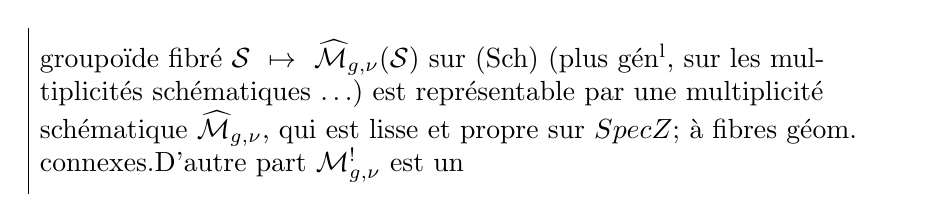
\begin{tikzpicture}
\node[anchor=north west,text width=0.9\linewidth,align=left,inner sep=4pt] (T) at (0,0) {
groupoïde fibré $\mathcal S\mapsto\widehat{\mathcal M}_{g,\nu}(\mathcal S)$ sur $(\mathrm{Sch})$ (plus gén\textsuperscript{l}, sur les multiplicités schématiques $\ldots$) est représentable par une multiplicité schématique $\widehat{\mathcal M}_{g,\nu}$, qui est \uline{lisse} et \uline{propre} sur $\operatorname{Spec}\mathbb Z$; \deleted{à fibres géom. connexes.}\inserted{D'autre part $\mathcal M^!_{g,\nu}$ est un}
};
\draw[line width=0.5pt] (T.north west)--(T.south west);
\end{tikzpicture}}
\mspage{23}
\scanpage{25}
\figure{
\begin{tikzpicture}
\node[anchor=north west,text width=0.9\linewidth,align=left,inner sep=4pt] (T) at (0,0) {
ouvert de Zariski de $\widehat{\mathcal M}_{g,\nu}$, schématiquement dense fibre par fibre.
};
\draw[line width=0.5pt] (T.north west)--(T.south west);
\end{tikzpicture}}

On en déduit aisément p.ex. la connexité des fibres géom. de $\mathcal M_{g,\nu}$ en toute car., à partir de \deleted{\unsure{la}} \unsure{connexité} en car. $0$. D'autre part, pour $\forall$ type $[G]$ de MD-graphe, ayant le type numérique $(g,\nu)$, les courbes \unsure{standard|standart} de type $[G]$ (sur une base quelc. $\mathcal S$) sont manifestement des MD-courbes relatives de type numérique $(g,\nu)$. On en conclut un morphisme canonique
\[
(25)\qquad\mathcal M_{[G]}\hookrightarrow\widehat{\mathcal M}_{g,\nu}
\]
dont on vérifie aisément que c'est une \uline{immersion}. Le cas où $G$ est le
\mspage{24}
\scanpage{26}
\mspage{12}
MD-graphe trivial, ayant un seul sommet de genre $g$, de poids marqué $\nu$, et pas d'arêtes, redonne l'immersion ouverte canonique
\[
(26)\qquad\mathcal M_{g,\nu}\hookrightarrow\widehat{\mathcal M}_{g,\nu}.
\]
Identifiant les $\mathcal M_{[G]}$ à des sous-multiplicités de $\widehat{\mathcal M}_{g,\nu}$, on voit que les $\mathcal M_{[G]}$ (pour tous les types de \unsure{MD}-graphes possibles, de type numérique $g,\nu)$) forment une \uline{partition} de $\widehat{\mathcal M}_{g,\nu}$ en un nb fini de sous-multiplicités.

\uline{Remarque} Considérons l'adhérence d'un $\mathcal M_{[G]}$ dans $\widehat{\mathcal M}_{g,\nu}$, on trouve que c'est une réunion finie de $\mathcal M_{[G']}$. On dit que $[G']$ est spécialisation de $[G]$ si $\mathcal M_{G'}\subset\overline{\mathcal M}_G$ dans $\widehat{\mathcal M}_{g,\nu}$.
\mspage{25}
\scanpage{27}
C'est là une \uline{relation d'ordre} dans l'ens des classes d'iso. de MD-graphes de type numérique $(g,\nu)$, ayant un plus grand élément. Dans la suite, nous allons préciser considérablement cette notion de spécialisation entre MD-graphes, en la reliant à une notion de \uline{morphismes} (de ``générisation'') de MD-graphes.

Notons que chaque $\mathcal M_{[G]}$ \deleted{\unsure{est donné}}\inserted{admet} un revêt\textsuperscript{t} fini $\mathcal M_G$, qui est représentable comme produit fini
\[
\mathcal M_G\simeq\prod_\alpha\underbrace{\mathcal M_{g_\alpha,\widehat I_\alpha}}_{\text{dim }3(g_\alpha-1)+\widehat\nu_\alpha}
\]
donc
\[
\deleted{\unsure{(26)}}(27)\quad\begin{aligned}
\dim\mathcal M_G/\mathbb Z&=\sum_{\alpha\in S}3(g_\alpha-1)+\sum\widehat\nu_\alpha\\
&=3\sum g_\alpha-3\underbrace{\operatorname{card}S}_{s_0}+\sum_{\alpha\in S}\underset{\substack{|\\\text{poids}\\\text{marqué}}}{\nu_\alpha}+\sum_{\alpha\in S}\underset{\substack{|\\\text{ordre}}}{\unsure{\widetilde\mu_\alpha}}\\
&=3\sum g_\alpha-3s_0+\nu+2s_1
\end{aligned}
\]
\mspage{26}
\scanpage{28}
\mspage{13}
où $s_0,s_1$ sont resp. les nbs de sommets et d'arêtes du graphe $G$. Or
\[
-3s_0+2s_1=-3(\underbrace{s_0-s_1}_{1-h_1})-s_1=-3+3h_1-s_1=3(h_1-1)-s_1
\]
d'où
\[
\dim\mathcal M_G/\mathbb Z=3(\underbrace{(\sum g_\alpha)+h_1}_{g}-1)+\nu-s_1
\]
et enfin la formule
\[
(\unsure{28})\qquad\dim\mathcal M_G/\mathbb Z=\underbrace{[3(g-1)+\nu]}_{=\dim\widehat{\mathcal M}_{g,\nu}/\mathbb Z}-s_1,
\]
i.e.
\[
(\unsure{29})\qquad\operatorname{codim}_{\widehat{\mathcal M}_{g,\nu}}\mathcal M_{[G]}=s_1
\]
(nb d'arêtes du MD-graphe $G$, i.e. ``nb de pts doubles'' des courbes \unsure{standard|standart} de type $G$).

L'entier (27) est appelé \uline{dimension modulaire} du MD-graphe $G$
\[
30)\qquad\begin{aligned}
\mu(G)&=\sum_{\alpha\in S}(3g_\alpha-1)+\widehat\nu_\alpha)=3\sum g_\alpha-3s_0+\nu+2s_1\\
&=(3(g-1)+\nu)-s_1,
\end{aligned}
\]
l'entier $s_1=\operatorname{card}A=(\operatorname{card}\widetilde A)/2$ s'appelle la codimension modulaire. Elle est nulle sss $G$ est un MD-graphe trivial (réduit à un pt isolé, sans arêtes, mais
\mspage{27}
\scanpage{29}
avec un poids marqué $\unsure{\nu}$, et bien sûr, un genre donné). Du pt de vue \unsure{structure} de graphe associé au type numérique $g,\nu)$, c'est le plus simple de tous ! On étudiera les plus complexes tantôt, qui correspondent au cas d'une dimension modulaire nulle, \unsure{ou} d'une codimension modulaire maximale, égale à $3(g-1)+\nu$.

Il est tentant d'introduire le compactifié
\[
\widehat{\mathcal M}_G\overset{\mathrm{déf}}{=}\prod_{\alpha\in S}\widehat{\mathcal M}_{g_\alpha,\widehat I_\alpha}
\]
où les $\widehat{\mathcal M}_{g_\alpha,\widehat I_\alpha}$ sont les compactifiés de MD des $\mathcal M_{g_\alpha,\widehat I_\alpha}\simeq\mathcal M_{g_\alpha,\widehat\nu_\alpha}$. \deleted{\unsure{Ils|Il}}\inserted{Pour $\alpha$ fixé, $\widehat{\mathcal M}_{g_\alpha,\widehat I_\alpha}$} \unsure{représente|représentent} le groupoïde fibré
\[
(30)\qquad\begin{aligned}
\mathcal S\longmapsto&\ \text{courbes de MD relatives }\inserted{Y_\alpha}\text{ sur }\mathcal S,\\
&\text{de type }g_\alpha,\widehat I_\alpha\quad\text{i.e. de genre}\\
&g_\alpha,\text{ munies d'un mono}\\
&(\widehat I_\alpha)_{\mathcal S}\hookrightarrow Y_\alpha^{\text{lisse}}
\end{aligned}
\]
de sorte que $\widehat{\mathcal M}_G$ représente le groupoïde fibré
\mspage{28}
\scanpage{30}
\mspage{14}
\[
(31)\qquad\begin{aligned}
\mathcal S\longmapsto&\ \text{groupoïde des }\inserted{\text{systèmes }(Y_\alpha)_{\alpha\in S}\text{ de }}\text{courbes de MD}\\
&\inserted{Y_\alpha\text{ de genre }g_\alpha,}\ \text{\deleted{\unsure{à}} sur }\mathcal S,\text{ munies de mono.}\\
&\widehat I_{\alpha\mathcal S}\hookrightarrow Y_\alpha^{\text{lisse}}.
\end{aligned}
\]
Posant alors
\[
\underset{\text{\deleted{On aura}}}{(32)}\qquad\left\{\begin{aligned}
\widehat I&=\coprod\widehat I_\alpha\simeq I\amalg\widetilde A\\
Y&=\coprod_{\alpha\in S}Y_\alpha
\end{aligned}\right.
\]
on aura un mono
\[
(33)\qquad\widehat I_{\mathcal S}\hookrightarrow Y^{\text{lisse}}
\]
qui permet, d'une part de construire un
\[
(34)\qquad\overset{\deleted{\unsure{\wedge}}}{\mathcal X}=Y/\unsure{(\sigma)_{\widetilde A_{\mathcal S}}|(\sigma_{\widetilde A_{\mathcal S}})},
\]
qui sera manifestement une courbe \deleted{\unsure{standard|standart}\inserted{MD}} sur $\mathcal S$, et d'autre part de définir
\[
(35)\qquad\overset{\deleted{\unsure{\wedge}}}{I}_{\mathcal S}\hookrightarrow\overset{\deleted{\unsure{\wedge}}}{\mathcal X}^{\text{lisse}}
\]
de sorte que $(\mathcal X,\overset{\deleted{\unsure{\wedge}}}{I}_{\mathcal S})$ devient une courbe \deleted{\unsure{standard|standart} sur $\mathcal S$} MD sur $\mathcal S$, ``épinglée'' par l'ens fini $I$. On a donc un morphisme canonique de multiplicités
\[
(36)\qquad\widehat{\mathcal M}_G\longrightarrow\widehat{\mathcal M}_{g,I}
\]
\margin{\uline{NB} Ce morphisme est une imm. locale, mais pas une immersion [il ne correspond pas à un morphisme \unsure{pl. fid.|rel. fid.} des \unsure{gr.} \unsure{à priori définis}].}
compatible d'ailleurs avec l'action de $\Gamma=\operatorname{Aut}G$ sur $\widehat{\mathcal M}_G$, et son action sur $\widehat{\mathcal M}_{g,I}$ via $\Gamma\to\unsure{\mathfrak S_I|\mathfrak G_I}$.
\mspage{29}
\scanpage{31}
On en déduit donc un morphisme can. de multiplicités schématiques
\[
(37)\qquad
\diagram{\begin{tikzcd}[column sep=large,row sep=small]
\widehat{\mathcal M}_{[G]}\arrow[r,hook]&\widehat{\mathcal M}_{g,\nu}\\
(\widehat{\mathcal M}_G,\Gamma)\arrow[u,phantom,"{\unsure{\wr|=}\ \mathrm{déf}}" description] & (\widehat{\mathcal M}_{g,I},\unsure{\mathfrak S_I|\mathfrak G_I})\arrow[u,phantom,"{\unsure{\wr|=}}" description]
\end{tikzcd}}
,
\]
qui est encore une \uline{immersion}, fermée cette \unsure{fois|fois-ci}, de multiplicités schématiques propres et lisses sur $\mathbb Z$. Ainsi se trouve \unsure{explicité|explicitée} l'adhérence de $\mathcal M_{[G]}$ dans $\widehat{\mathcal M}_{g,\nu}$, comme sous-multiplicité propre et lisse sur $\operatorname{Spec}\mathbb Z$ -- qui \unsure{paraît} \inserted{a priori} curieux ! En $\unsure{=|\overline m}$ temps, cette construction permet de décrire de façon pratiquement triviale les types $[G']$ qui sont spécialisation de $[G]$, puisque ce sont ceux qui proviennent de $\widehat{\mathcal M}_G$. Nous allons \deleted{\unsure{y}} revenir là dessus maintenant.
\mspage{30}
\scanpage{32}
\mspage{15}
5. \uline{Spécialisation \deleted{et générisation} de MD-graphes.}

Soit
\figure{\begin{tikzpicture}[baseline=(f.base)]
\node[inner sep=7pt] (f) {$(38)\quad G=(S,\widetilde A,\sigma_{\widetilde A},\deleted{\unsure{\widetilde A|A}}I,\ \underset{\substack{\Vert\\\widetilde A\amalg I}}{\widehat I}\to S\xrightarrow[g]{}\deleted{\unsure{g}}\mathbb N)$};
\draw ([xshift=-.5cm]f.south west)--(f.south west)--(f.north west)--(f.north east)--(f.south east)--([xshift=.1cm]f.south east);
\end{tikzpicture}}
un MD-graphe, de type numérique $(g,\nu)$. Nous allons construire ses \deleted{$\unsure{G}$} spécialisations, comme les \inserted{MD-}graphes associés aux diverses ``strates'' de
\[
\deleted{\unsure{\widehat{\mathcal M}_G}}\qquad\widehat{\mathcal M}_G=\prod_{\alpha\in S}\widehat{\mathcal M}_{g_\alpha,\widehat I_\alpha}.
\]
Une telle strate est obtenue en choisissant, pour $\forall\ \alpha$, une strate de $\widehat{\mathcal M}_{g_\alpha,\widehat I_\alpha}$, c'est à dire une classe d'isomorphie de MD-graphe
\deleted{$G_\alpha=(S_{(\alpha)},\widetilde A_{(\alpha)},\sigma_{\widetilde A_{(\alpha)}},\ I_{(\alpha)}=\widehat I_\alpha\to S_{(\alpha)}\to\mathbb N)$ de type numérique}
de type \deleted{$(g_\alpha,\widehat\nu_\alpha)$} numérique $(g_\alpha,\widehat I_\alpha)$
\[
(39)\quad\deleted{\unsure{(g_\alpha,\widehat\nu_\alpha)}}.\quad
\begin{aligned}
G_{(\alpha)}=(S_{(\alpha)},\widetilde A_{(\alpha)},\sigma_{\widetilde A_{(\alpha)}},\ &I_{(\alpha)}=\widehat I_\alpha,\\
&\deleted{\unsure{I_{(\alpha)}\amalg\widetilde A_{(\alpha)}\to S_{(\alpha)}\xrightarrow{g_\alpha}\mathbb N}}\\
&\inserted{\widehat I_{(\alpha)}\overset{\mathrm{déf}}{=}\widetilde A_{(\alpha)}\amalg I_{(\alpha)}\to S_{(\alpha)}\xrightarrow{\unsure{g_\alpha|\sigma_\alpha}}\mathbb N})
\end{aligned}
\]
(\uline{NB} bien entendu, le cas où $G_{(\alpha)}$ est le MD-graphe trivial de type $(g_\alpha,\widehat\nu_\alpha)$ n'est pas exclu).

Par ``classes d'isomorphie'', il faut entendre ici : pour des isomorphismes induisant l'identité sur $I_{(\alpha)}=\widehat I_\alpha$. Au lieu de travailler avec de telles classes d'isomorphie, nous allons pour commencer travailler
\mspage{31}
\scanpage{33}
avec ces $G_{(\alpha)}$ eux-mêmes.

Le \inserted{MD-}graphe \inserted{$G'$} spécialisé de $G$ associé aux $G_{(\alpha)}$ s'obtient ainsi :
\[
(40)\quad\left\{\begin{aligned}
S'&=\coprod_{\alpha\in S}S_{(\alpha)}\\
\widetilde A'&=\widetilde A\amalg\coprod_{\alpha\in S}\widetilde A_{(\alpha)}\\
\sigma_{\widetilde A'}&\quad\text{induit par }\sigma_{\widetilde A}\text{ et par les }\sigma_{\widetilde A_{(\alpha)}}\\
&\deleted{\unsure{\widetilde A'}}\\
I'&=I\quad\text{donc }\begin{aligned}[t]
&\inserted{\widehat I'\overset{\mathrm{déf}}{=}}\widetilde A'\amalg I'\simeq\underbrace{(\widetilde A\amalg I)}_{\widehat I\simeq\coprod_{\alpha\in S}\widehat I_\alpha=\coprod_{\alpha\in S}I_{(\alpha)}}\amalg\coprod_{\alpha\in S}\widetilde A_{(\alpha)}\\
&\deleted{\unsure{=}}\simeq\coprod_{\alpha\in S}\underbrace{\widehat I_\alpha\amalg\widetilde A_{(\alpha)}}_{I_{(\alpha)}}
\end{aligned}\\
&\deleted{\unsure{\widehat I'\amalg\widetilde A'|I'\amalg\widetilde A'}}.\\
\widehat I'&\to S'\quad\text{induit par les }\widehat I_{(\alpha)}\to S_{(\alpha)}\\
S'&\xrightarrow{g'}\mathbb N\quad\text{induit par les }S_{(\alpha)}\xrightarrow{\deleted{\unsure{g_\alpha}}}\mathbb N
\end{aligned}\right.
\]
Donc ``la ''recette \inserted{pratique''} est la suivante :

\deleted{\unsure{y}} On remplace chaque sommet \inserted{$\alpha\in S$} de $G$ par un MD-graphe $G_{(\alpha)}$, de type numérique $(g_\alpha,\widehat\nu_\alpha)$, où $\widehat\nu_\alpha=\nu_\alpha+\widetilde\mu_\alpha$ ($\nu_\alpha=\operatorname{card}I_\alpha$, poids marqué de $\alpha$, $\unsure{\widehat\mu_\alpha|\widetilde\mu_\alpha}=\text{ordre de }\alpha=\text{nb de}\allowbreak\text{ arcs de }G\text{ sortant de }\alpha$), plus précisément, un MD-graphe de type $(g_\alpha,\widehat I_\alpha)$, où $\widehat I_\alpha=I_\alpha\amalg\widetilde A_\alpha$.
\mspage{32}
\scanpage{34}
\mspage{16}
Cela signifie qu'on se donne, pour $\alpha$ fixé,

1°) un graphe \inserted{connexe} $(S_{(\alpha)},\widetilde A_{(\alpha)},\deleted{\unsure{\widetilde A_{(\alpha)}}}\sigma_{\widetilde A_{(\alpha)}},\widetilde A_{(\alpha)}\to S_{(\alpha)})$

2°) on \deleted{\unsure{se}} donne une application ``genre''
\[
S_{(\alpha)}\xrightarrow{\unsure{\gamma_\alpha|g_\alpha}}\mathbb N
\]

3°) on donne une application $I_\alpha\to S_{(\alpha)}$, i.e. on ``répartit'' les \deleted{\unsure{divers}} ``pts marqués'' au dessus de $\alpha$ \inserted{(i.e. les éléments de $I_\alpha$)} entre les sommets $\beta\in S_{(\alpha)}$ de $G_{(\alpha)}$

4°) on donne une application $\widetilde A_\alpha\to S_{(\alpha)}$, i.e. pour $\forall$ \deleted{flèche}\inserted{arc} du graphe $G$, d'origine $\alpha$, on \deleted{\unsure{se donne}} choisit une \inserted{nouvelle} ``origine'' parmi les sommets $\beta\in S_{(\alpha)}$ du graphe $G_{(\alpha)}$

5°) Les données 1°) : 4°) définissent une maquette, \inserted{0-connexe, $G_{(\alpha)}$} et on prend soin que celle-ci soit un MD-graphe, \deleted{\unsure{ce}} ce qui signifie ici pour pour $\forall\beta\in S_{(\alpha)}$ ``de genre 0'' i.e. tel que $\unsure{\gamma_\alpha|g_\alpha}(\beta)=0$, on ait $\operatorname{card}I_{\alpha,\beta}+\operatorname{card}\widetilde A_{\alpha,\beta}\geq 3$.

Ceci étant, on trouve un nouveau \inserted{MD-}graphe\inserted{$G'$}, \inserted{qui sera} spécialisé du \inserted{MD-}graphe $G$.

Je voudrais préciser de façon symétrique la relation entre les MD-graphes $G$ et $G'$, et j'introduis à cet effet une digression sur
\mspage{33}
\scanpage{35}
une \unsure{extension|catégorie} de la notion de \uline{morphismes de graphes}.

\deleted{\unsure{6}}\qquad\deleted{Soit}

6. \uline{Morphismes de générisation de graphes \deleted{\unsure{quelconques}}\inserted{et de maquettes}}

Soit $G=(S,\widetilde A,\sigma_{\widetilde A},o_{\widetilde A}:\widetilde A\unsure{\to|{-}}S)$ un graphe ordinaire. On lui associe de façon bien connue un \uline{groupoïde fondamental} \inserted{$\Pi_1(G)$}, dont l'ens des objets est $S$, et l'ens des \deleted{\unsure{chemins de}}\inserted{morphismes} de $s$ à $s'$ est l'ens des ``chemins simples'' de $s$ à $s'$, qui correspondent aux classes d'homotopie de chemins de $s$ à $s'$ dans la réalisation topologique du graphe $G$. Le groupoïde $\Pi_1(G)$ dépend fonctoriellement (au sens le plus strict !) du graphe $G$.

D'ailleurs, un morphisme de graphes
\[
(41)\qquad f:G'\longrightarrow G^{\deleted{\unsure{'}}}
\]
\mspage{34}
\scanpage{36}
\mspage{17}
est connu quand on connaît
\[
(42)\qquad\Pi_1(f):\Pi_1(G')\longrightarrow\Pi_1(G^{\deleted{\unsure{'}}}),
\]
puisqu'alors on connaît l'action de $f$ sur $S$ via l'action de $\Pi_1(f)$ sur les objets, et l'action de $f$ sur les arcs via l'action de $\Pi_1(f)$ sur les flèches, grâce au diagramme comm.

(43)\quad\diagram{\begin{tikzcd}
\widetilde A(G')\arrow[r,"\widetilde A(f)"]\arrow[d,hook]&\widetilde A(G)\arrow[d,hook]\\
\operatorname{Fl}(\Pi_1(G'))\arrow[r,"\operatorname{Fl}(\Pi_1(f))"]&\operatorname{Fl}(\Pi_1(G))
\end{tikzcd}}.

En fait, les morphismes de $G$ dans $G'$ s'identifient aux morphismes de groupoïdes $\Pi_1(G')$ dans $\Pi_1(G)$, qui transforment arcs \inserted{de $G'$} en arcs de $G$.

Ceci étant, on généralise la notion de morphisme de graphes en celle de \uline{morphisme généralisé} de $G'$ dans $G^{\deleted{\unsure{'}}}\deleted{\unsure{,}}$, (ou ``\uline{morphisme de générisation}'' de $G'$ dans $G^{\deleted{\unsure{'}}}$)
\mspage{35}
\scanpage{37}
comme étant les morphismes de groupoïdes $\Pi_1(G')\unsure{\to|{-}}\Pi_1(G^{\deleted{\unsure{'}}})$ qui transforment tout arc de $G'$ en une flèche de $\Pi_1(G)$ qui est, \uline{soit} un arc de $G^{\deleted{\unsure{'}}}$, soit une flèche identique. En d'autres termes, appelant \uline{flèche élémentaire} de $\Pi_1(G')$ $\forall$ flèche qui est, soit identique, soit un arc de $G'$ (ensemble \inserted{de flèches} stable par passage à la flèche opposée\ldots), les morphismes \deleted{de} \deleted{\unsure{générisation}}\inserted{\unsure{généralisés}} de $G'$ dans $G^{\deleted{\unsure{'}}}$ sont les morphismes de $\Pi_1(G')$ dans $\Pi_1(G)$ qui transforment fls élémentaires en fl. élémentaires. Cette description a l'avantage de rendre évident que cette notion est stable par composition.

Pratiquement, la donnée d'un morphisme \deleted{de} \deleted{\unsure{générisation}}\inserted{\unsure{généralisé}} \deleted{\unsure{de}} $G'\longrightarrow G^{\deleted{\unsure{'}}}$ est \unsure{définie|défini}
\mspage{36}
\scanpage{38}
\mspage{18}
par une application
\[
(44)\qquad S'\amalg\widetilde A'\longrightarrow S^{\deleted{\unsure{'}}}\amalg\widetilde A^{\deleted{\unsure{'}}}
\]
qui applique $S'$ dans $S^{\deleted{\unsure{'}}}$ (mais pas néc. $\widetilde A'$ dans $\widetilde A^{\deleted{\unsure{'}}}$), qui commute à $\sigma_{G'}$ et $\sigma_{G^{\deleted{\unsure{'}}}}$ (définis via $\sigma_{\widetilde A'}$ et $\sigma_{\widetilde A^{\deleted{\unsure{'}}}}$, avec l'identité sur $S'$ resp. $S^{\deleted{\unsure{'}}}$) et commute à l'application ``origine'' (qui sur $S'$ resp. $S^{\deleted{\unsure{'}}}$ est l'identité).

On peut aussi dire que c'est défini par la donnée
\[
(45)\quad\left\{\begin{aligned}
&\text{1°) d'une application}\qquad f_{\unsure{S|S^0}}:S'\longrightarrow S^{\deleted{\unsure{'}}}\\
&\text{2°) d'une partie }\deleted{\unsure{\widetilde A}}\widetilde B'^{\deleted{\unsure{'}}}\text{ de }\widetilde A',\text{ stable par }\sigma_{\widetilde A'}\\
&\text{3°) d'une application }\widetilde B'\unsure{\to|{-}}\widetilde A^{\deleted{\unsure{'}}}\text{ commutant à }\deleted{\unsure{\sigma}}\\
&\qquad\sigma_{\widetilde A'}|\widetilde B'\text{ et à }\sigma_{\widetilde A^{\deleted{\unsure{'}}}},\text{ et aux applications}\\
&\qquad o_{\widetilde A'}|\widetilde B'\text{ et }o_{\widetilde A^{\deleted{\unsure{'}}}}.
\end{aligned}\right.
\]
\margin{et il faut supposer de plus que pour $\forall\vec a\in\widetilde A'\setminus\widetilde B'$, l'origine et l'extrémité de $\vec a$ ont $\unsure{\overline m|=}$ image dans $S$ par $f_S$}

On peut dire enfin que c'est aussi la donnée d'un sous-graphe $G_{\widetilde B'}$ de \deleted{\unsure{$G$}}$G'$ ayant $\unsure{=_{\mathrm s}|\overline m_{\mathrm s}}$ sommets (cela \unsure{définir|définit} juste \unsure{rev.|un} à donner une partie $\widetilde B'$ de $\widetilde A'$ stable par $\sigma_{\widetilde A'}$), et un morphisme de $G_{\widetilde B'}$ dans $G^{\deleted{\unsure{'}}}$. La composition des morphismes généralisés est alors définie et lue de façon
\mspage{37}
\scanpage{39}
évidente. Ainsi on trouve la catégorie \unsure{étendue} des graphes, dont les objets sont les graphes, les \deleted{morphismes}\inserted{flèches} les morphismes généralisés de graphes. On notera que les iso. dans cette nouvelle catégorie sont les iso au sens ordinaire.

Supposons maintenant que $G',G^{\deleted{\unsure{'}}}$ fassent partie de MD-graphes \inserted{$\underline G',\underline G^{\deleted{\unsure{'}}}$}, i.e. soient munis de plus de \deleted{$\unsure{S}\xrightarrow{\unsure{g}}\mathbb N$},
\[
(46)\quad\left\{\begin{aligned}
&S\overset{\underline g}{\unsure{\longrightarrow|{-}}}\mathbb N,\qquad S'\xrightarrow{\underline{g'}}\mathbb N\\
&I\longrightarrow S,\qquad I'\longrightarrow S'
\end{aligned}\right.
\]
On dit qu'on a un \uline{morphisme de générisation} de $\underline G'$ dans $\underline G^{\deleted{\unsure{'}}}$, si on se donne, en plus du morphisme \inserted{généralisé} $G'\unsure{\to|{-}}G^{\deleted{\unsure{'}}}$, une application bijective
\[
(47)\qquad I'\xrightarrow{\sim}I^{\deleted{\unsure{'}}},
\]
\deleted{\unsure{satisfai|satisfa}} et si les conditions suivantes sont satisfaites :
\mspage{38}
\scanpage{40}
\mspage{19}
a) $S'\longrightarrow S^{\deleted{\unsure{'}}}$ surjectif, $\widetilde B'\longrightarrow\widetilde A^{\deleted{\unsure{'}}}$ \uline{bijectif}

b) \diagram{\begin{tikzcd}
I'\arrow[r,"\sim"]\arrow[d]&I\arrow[d]\\
S'\arrow[r]&S
\end{tikzcd}} commutatif

\margin{donc \diagram{\begin{tikzcd}
\widetilde B'\amalg I'\arrow[r,"\sim"]\arrow[d]&\widetilde A\amalg I\arrow[d]\\
S'\arrow[r]&S
\end{tikzcd}} est comm.}

c) $\forall\alpha\in S$, le sous-graphe $G'(\alpha)$ de $G'$ [formé des \deleted{\unsure{$S$}} $s'\in S'$ au dessus de $\alpha$, et des \deleted{flèches} arcs $a'\in\widetilde A'$ qui sont dans $\inserted{\widetilde C'=}\widetilde A'\setminus\widetilde B'$ (i.e. au dessus de $\operatorname{id}_\alpha$) et dont l'origine (donc l'extrémité \inserted{$(^{+})$} aussi) est dans $S'_\alpha$], muni de \deleted{\unsure{$\widetilde A$}\unsure{ et }\unsure{$A$}} $I'_\alpha\inserted{\amalg\unsure{\widetilde B'_\alpha}}\longrightarrow S'_\alpha$ induit par $\inserted{\widetilde B'\amalg}I'\unsure{\to|{-}}S'$, et de $\gamma_\alpha:S'_\alpha\longrightarrow\mathbb N$ induit par $g':S'\unsure{\to|{-}}\mathbb N$, est un \uline{MD-graphe} \inserted{$\underline G'(\alpha)$} \deleted{\unsure{de type|de genre} $\unsure{g=g(\alpha)|(g_\alpha,\nu_\alpha)}$\unsure{, i.e.}}, i.e. il est \uline{connexe}, \deleted{[NB il \unsure{satisfait automatiquement}} \inserted{et [il satisfait \unsure{tous}}\deleted{\unsure{les}} \inserted{les} conditions de rigidité relatives aux sommets $\beta$ tels que, \deleted{\unsure{$\alpha$}} $g'_\beta\in\{0,1\}$, à savoir que

\margin{\uline{NB} $\widetilde B'_\alpha$ est l'ens des $\vec a'\in\widetilde B'_\alpha$ dont l'origine se trouve dans $S'_\alpha$, i.e. dans $G'(\alpha)$, donc $\widetilde B'_\alpha\xrightarrow{\sim}\widetilde A_\alpha$}

\figure{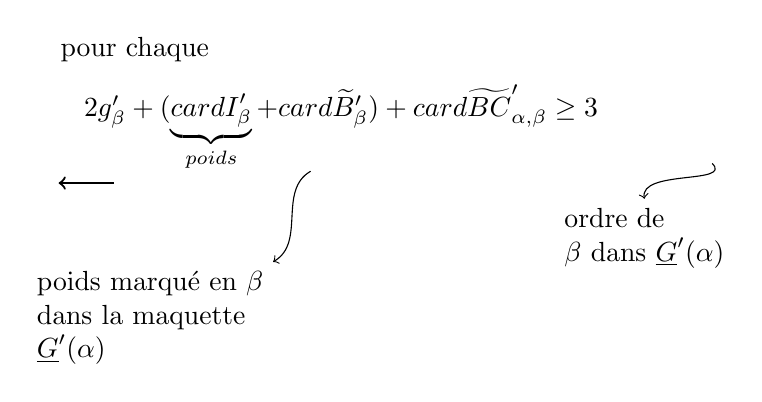
\begin{tikzpicture}[x=1cm,y=1cm]
\node[anchor=west] (eq) at (0,0) {$2g'_\beta+(\underbrace{\operatorname{card}I'_\beta}_{\deleted{\unsure{poids}}}\inserted{+\operatorname{card}\widetilde B'_\beta)}+\operatorname{card}\widetilde{\deleted{B}\inserted{C}}'_{\deleted{\unsure{\alpha}},\beta}\geq3$};
\node[anchor=north west,align=left] (mark) at (-0.6,-1.7) {poids marqué en $\beta$\\dans la maquette\\$\underline G'(\alpha)$};
\node[anchor=north west,align=left] (ord) at (6.1,-0.9) {ordre de\\$\beta$ dans $\underline G'(\alpha)$};
\draw[->,thick] (0.5,-0.7)--(-0.2,-0.7);
\draw[->] (3.0,-0.55) to[out=210,in=30] (mark.north east);
\draw[->] (8.1,-0.45) to[out=-45,in=100] (ord.north);
\node[anchor=west] at (-0.3,1.0) {\deleted{\unsure{pour chaque}}};
\end{tikzpicture}}

\margin{\unsure{car la condition est aut. assur.} \deleted{\unsure{a priori} $\unsure{2g'_\beta}$ \unsure{est}} \deleted{\unsure{puisqu'il est}} \unsure{équiv à} : \figure{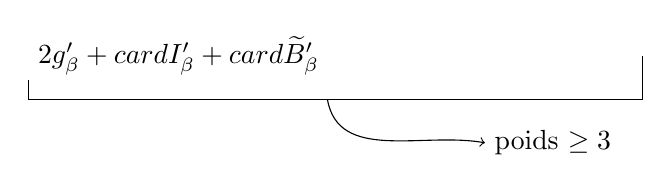
\begin{tikzpicture}[x=1cm,y=1cm]
\node[anchor=west] at (0,0) {$2g'_\beta+\operatorname{card}I'_\beta+\operatorname{card}\widetilde B'_\beta$};
\draw (0,-0.3)--(0,-0.55)--(7.8,-0.55)--(7.8,0);
\draw[->] (3.8,-0.55) to[out=-80,in=170] (5.8,-1.1);
\node[anchor=west] at (5.8,-1.1) {poids $\geq3$};
\end{tikzpicture}}}

\deleted{\unsure{qui a priori} \unsure{$+\operatorname{car}$} $\left[2g'_\beta+\operatorname{card}I'_\beta\geq3\right]$ $2g'_\beta+\operatorname{card}I'_\beta+\operatorname{card}\widetilde A'_\beta\geq3)$ qui a priori est une condition plus faible (puisque $\underline G'$ est un MD-graphe)\ldots}

d) le genre du MD-graphe $\underline G'(\alpha)$ est égal à $g_\alpha$, i.e. on a
\[
\sum_{\beta\in S'_\alpha}\unsure{g'_\beta|\gamma'_\beta}+h_1(G'(\alpha))=g_\alpha.
\]
\mspage{39}
\scanpage{41}
\uline{NB} Pour qu'un morphisme généralisé de graphes $G'\deleted{\unsure{\text{et}}}\longrightarrow G$ corresponde à un morphisme de générisation (pour $I'\simeq I$ convenable), il f. et s. qu'il satisfasse aux conditions suivantes
\[
(48)\quad\left\{\begin{aligned}
&\text{1°) }S'\unsure{\to|{-}}S\text{ surjectif},\quad\widetilde B'\longrightarrow\widetilde A\text{ bijectif, les}\\
&\qquad\inserted{\text{``graphes}}\text{ fibres'' }G'(\alpha)\quad(\alpha\in S)\text{ connexes. (Ces}\\
&\qquad\text{conditions ne dépendent pas des MD-}\\
&\qquad\text{structures sur }G',G\text{)}\\[1em]
&\text{2°) }\forall\alpha\in S,\text{ on a}\\
&\qquad\underbrace{\operatorname{card}I_\alpha}_{\nu_\alpha}=\sum_{\beta\in S'_\alpha}\underbrace{\operatorname{card}I'_\beta}_{\nu'_\beta}\\
&\qquad\text{(cette condition ne dépend que des}\\
&\qquad\text{``poids marqués'' sur }\unsure{\widehat S|S},S',\text{ et bien sûr}\\
&\qquad\text{de }S'\unsure{\to|{-}}S\text{)}\\[1em]
&\unsure{\text{3°)}}\quad\forall\alpha\in S,\text{ on a}\\
&\qquad g_\alpha=\Big(\sum_{\beta\in S'_\alpha}g'_\beta\Big)+h_1(G'(\alpha))\\[1em]
&\deleted{\unsure{\text{4°)}}\quad\forall\unsure{\beta|\alpha'}\in S',\text{ on a (non seulement}}\\
&\deleted{\quad2g'_{\alpha'}+\operatorname{card}I'_{\alpha'}+\operatorname{card}\widetilde A'_{\beta'}\geq3,\text{ mais même)}}\\
&\deleted{\qquad\unsure{2|7}g'_{\alpha}+\operatorname{card}I'_{\alpha'}+\operatorname{card}\unsure{\widetilde C'|\widetilde B'}_{\alpha'}\geq3}
\end{aligned}\right.
\]
\mspage{40}
\scanpage{42}
\mspage{20}
Reprenons un morphisme généralisé de graphes ordinaires $f:G'\to G^{\deleted{\unsure{'}}}$. On dit que $f$ est un \uline{morphisme de générisation} s'il satisfait la condition 1°) de (48). Notons que $G$ et $f$ sont définis alors à iso près par $G'$ et l'ens $\widetilde B'\subset\widetilde A'$ (stable par $\sigma_{\widetilde A'}$), ou ce qui revient au $\unsure{=|\overline m}$, par $G'$ et la \deleted{\unsure{ens}} partie $B'$ de $A'=\widetilde A'/\sigma_{\widetilde A'}$ ($B'$ est donc un ens. d'arêtes de $G'$). En effet, soit $G'_\bullet$ le sous-graphe de $G'$ défini par $S'$ et $A'\setminus B'\subset A'$ (ou $\widetilde A'\setminus\widetilde B'\subset\widetilde A'$) (i.e. \inserted{par $S'$ et} l'ens des \deleted{arêtes} arcs de $G'$ qui sont au dessus des identités de $\Pi_1(G)$). Alors il résulte de la condition $S'\unsure{\to|{-}}S$ surjectif et les $G'(\alpha)$ connexes ($\Longleftrightarrow$ les $G'(\alpha)$ 0-connexes) que \deleted{les fibres} l'homomorphisme canonique
\[
\pi_0(G'_\bullet)\longrightarrow S
\]
est bijectif, d'où
\[
(49)\qquad S\simeq\pi_0(G'_\bullet),
\]
d'ailleurs on a
\[
(50)\qquad\widetilde A\simeq\widetilde B'\qquad\unsure{\text{compatible}}\text{ avec }\sigma_{\widetilde B'}\text{ et }\sigma_{\widetilde A}
\]
\mspage{41}
\scanpage{43}
enfin $\widetilde A\xrightarrow{\unsure{o_G|\sigma_G}}S$ est donné par passage au quotient à partir de $o_G|\widetilde B':\widetilde B'\to S'$, par commutativité dans

(51)\quad\diagram{\begin{tikzcd}
\widetilde B'\arrow[r,"o_{G'}|\widetilde B'"]\arrow[d,"\unsure{\sim|\wr}"']&S'=\text{sommets de }G'_\bullet\arrow[d]\\
\widetilde A\arrow[r]&S\simeq\pi_0(G'_\bullet)
\end{tikzcd}}

Ainsi $G$ est reconstruit à partir de $G'$, et $f$ de $\unsure{\overline m|=}$ bien sûr. On voit que $G$ apparaît comme un quotient de $G'$, et en fait c'est plus une somme amalgamée dans la catégorie des graphes et des morphismes généralisés de graphes :

(52)\quad\diagram{\begin{tikzcd}[column sep=large,row sep=large]
G'_\bullet\arrow[r,hook,"\text{incl. can}"]\arrow[d,"\text{proj. can}"']\arrow[dr,phantom,"\text{cocart}"]&G'\arrow[d]\\
\begin{gathered}S=\pi_0(\unsure{G'_\bullet|S'_\bullet})\\
\text{Graphe }\deleted{\unsure{\text{ponctuel}}}\inserted{\text{discret}}\\
\text{défini par }S\overset{\mathrm{dfn}}{=}\pi_0(G'_\bullet)
\end{gathered}\arrow[r]&G
\end{tikzcd}}

i.e. $G'\longrightarrow G$ est universel parmi les morphismes généralisés de \inserted{$G$ dans un} graphe $G'$, qui transforment les arcs de $\widetilde A'\setminus\widetilde B'$ en des identités. Posons donc
\mspage{42}
\scanpage{44}
\mspage{21}
\[
(53)\qquad\widetilde C'=\widetilde A'\setminus\widetilde B',\qquad C'=A'\setminus B'=\widetilde C'/\sigma_{\widetilde A'},
\]
on écrira
\[
(54)\qquad G=G'/\widetilde C'\quad\text{ou}\quad G=G'/C'
\]
et on dira que $G$ \uline{est déduit de} $G'$ en contractant les arêtes $a'\in C'$ (ou encore, les arcs $\vec a'\in\widetilde C'$) en des pts. Interprétant les morphismes généralisés de graphes, en termes des réalisations \deleted{géométriques}\inserted{topologiques} de ceux-ci, à l'aide d'applications continues qui contractent juste certaines arêtes en des pts, on voit que cette terminologie correspond bien à une intuition topologique correcte. D'ailleurs la somme amalgamée (52) existe quel que soit le sous-graphe $G'_\bullet$ de $G'$ ayant $\unsure{=^{\mathrm s}|\overline m^{\mathrm s}}$ sommets que $G'$, i.e. quel que soit l'ens d'\deleted{flèches}\inserted{arêtes} $C'\subset A'$- de $G'_{\deleted{\unsure{\psi|\alpha}}\bullet}$. [Il s'ensuit que tout morphisme généralisé de graphes $G'\longrightarrow G$ se factorise de façon unique en un
\mspage{43}
\scanpage{45}
composé
\[
(55)\qquad G'\longrightarrow G_0\unsure{\longrightarrow|{-}}G,
\]
où $G'\unsure{\to|{-}}G_0$ est un morphisme de passage au quotient (par l'ens des arêtes de $G'$ contractées par $f$, justement) et où $G_0\longrightarrow G$ est un morphisme \inserted{ordinaire} de graphes.

Supposons maintenant que $G'$ \inserted{soit fixé, et} \deleted{soit} provienne \inserted{$\unsure{\overline m|=}$} d'un MD-graphe $\underline G'$, grâce aux données supplémentaires
\[
\deleted{\unsure{(55)|(56)}}\qquad I'\longrightarrow S',\xrightarrow{\unsure{g'|\underline{g'}}}\mathbb N,
\]
où $I'$ est un ens. fini. Alors $G$ provient canoniquement d'un MD-graphe $\underline G$, en posant $I=I_{\underline G}=I'$, et en définissant $\unsure{I|I'}\unsure{\to|{-}}S$ comme le composé
\[
\underset{\substack{\Vert\,\mathrm{déf}\\I}}{I'}\longrightarrow S'\unsure{\longrightarrow|{-}}S,
\]
et en définissant, pour $\forall\alpha\in S$
\[
(56)\qquad g_\alpha=\Big(\sum_{\alpha'\in\underset{\substack{\Vert\\\text{Sommets}\\\text{de }G'(\alpha)}}{S'_\alpha}}g'_{\alpha'}\Big)+h^1(G'(\alpha)).
\]
\mspage{44}
\scanpage{46}
\mspage{22}
Il faut cependant vérifier encore la condition MD sur la maquette $\underline G$ obtenue. Que $\underline G$ soit connexe résulte aussitôt de la connexité de $\underline G'$. Pour $\forall\alpha\in S$, il faut vérifier que
\[
2g_\alpha+\underbrace{\operatorname{card}I_\alpha+\operatorname{card}\widetilde A_\alpha}_{\widehat\nu_\alpha}\geq3
\]
\deleted{\unsure{or je dis qu'on aura mieux|ou je dis qu'on aura même}}

\deleted{ou}\inserted{i.e.} que $(g_\alpha,\widehat\nu_\alpha)$ est anabélien. Or
\[
\deleted{\operatorname{card}2g_\alpha+\operatorname{card}I_\alpha\geq3}
\]
\deleted{je dis}\inserted{on sait} que $(g_\alpha,\widehat\nu_\alpha)$ est le type numérique de la maquette $\underline{\unsure{G|G'}}(\alpha)$, dont le graphe sous-jacent est la composante connexe de $G'_\bullet$ correspondant à $\alpha$, et l'ens. des ``pts marqués'' est $I'_\alpha\amalg\deleted{\unsure{\widetilde A}}\inserted{\widetilde B}'_\alpha$, \deleted{\unsure{et|à}} où $I'_\alpha=I'|S'_\alpha\simeq I_\alpha$, et $\widetilde B'_\alpha=\deleted{\unsure{\widetilde B|\widetilde A}}\inserted{\unsure{\widetilde A|\widetilde B}}'_\alpha\cap\widetilde B'$ est l'ens des flèches $\in\widetilde B'$ d'origine dans $S'_\alpha$, l'hom de projection
\[
\unsure{I_{(\alpha)}|I^{(\alpha)}}^{\deleted{\unsure{\ast|\alpha}}}\overset{\mathrm{def.}}{=}I'_\alpha\amalg\widetilde B'_\alpha\longrightarrow S'_\alpha
\]
étant induit par $I'\to S'$ et l'application origine. Donc, en vertu de la prop. \unsure{de ce|du} n° 3, on aura $(g_\alpha,\widehat\nu_\alpha)$ anabélien pourvu qu'on sache que $\underline G(\alpha)$ est un MD-graphe. Mais cette condition signifie que l'on a, pour $\forall\beta\in S'_{\deleted{\unsure{\beta|\alpha'}}\inserted{\alpha}}$
\mspage{45}
\scanpage{47}
\[
2g'_\beta+\underbrace{\bigl(\operatorname{card}I'_\beta\deleted{\unsure{(\alpha)}}+\operatorname{card}\widetilde B'_{\unsure{\beta|\alpha}}\bigr)}_{\substack{\text{poids marqué}\\\text{de }\beta\text{ dans }\underline G(\alpha)}}+\underbrace{\operatorname{card}\widetilde C'_\beta}_{\substack{\text{ordre de}\\\beta\text{ dans }\underline G(\alpha)}}\geq3
\]
or cette expression s'écrit aussi, puisque
\[
\widetilde A'=\widetilde B'\amalg\widetilde C'
\]
\[
2g'_\beta+\underbrace{\operatorname{card}I'_\beta}_{\substack{\text{poids marqué}\\\text{de }\beta\text{ dans }\underline G'\deleted{\unsure{\alpha|\xi}}}}+\underbrace{\operatorname{card}\widetilde A_\beta}_{\substack{\text{ordre de }\beta\\\text{dans }\underline G'}}\geq3,
\]
et cette condition n'est autre que la condition \inserted{de rigidité} MD sur $\underline G'$.

Résumons les résultats sur les maquettes.

\uline{Proposition}\quad Soit
\[
\underline G'=\left(\underset{\substack{\Vert\\(S',\deleted{\unsure{\widetilde B}}\inserted{\widetilde A}',\sigma_{\widetilde A'},o_{\widetilde A'})}}{G'},\ I'\longrightarrow S'\xrightarrow{\unsure{g'|\underline{g'}}}\mathbb N\right)
\]
une maquette, et soit $C'\subset A'=\widetilde A'/\sigma_{\widetilde A'}$ un ens d'arêtes de $G'$. Alors on peut de façon unique \deleted{trouver} (à isom unique près) trouver un morphisme de générisation de maquettes
\[
\underline G'\longrightarrow\underline G
\]
\mspage{46}

% ===== MPL_147_048-137 (first pass) =====
\scanpage{48}
\mspage{23}
tel que $B$ soit l'ens des \unsure{arêtes} \inserted{de $\underline{G}'$} qui se ``contractent en un point''. On a
\[
\pi_0(G')\overset{\sim}{\longrightarrow}\pi_0(G)
\]
[donc $G$ est $0$-conn. ssi $G'$ l'est]. \deleted{Pour que} Soit, pour tt $\unsure{\alpha}\in S$ (ens des sommets de $\underline{G}$) $G'_\alpha$ le sous-graphe de $G'$ fibre en $\alpha$ (qui est une composante connexe du ss-graphe $G'_{\unsure{\cdot}}$ de $G'$ défini par $S'$ et $C'$)\deleted{$\unsure{=A'|C'}$}, et $\underline{G}'_\alpha$ le \unsure{m.graphe} déduit de $G'_\alpha$ en considérant l'application ``genre'' $S'_\alpha\mathbin{\text{---}}\mathbf{N}$ induite par $g':S'\mathbin{\text{---}}\mathbf{N}$, et en prenant comme ens de pts marqués $I'_\alpha\amalg\widetilde{B}'_\alpha$ (où $I'_\alpha=I'|S'_\alpha$,
\[
\widetilde{B}'=\widetilde{A}'\setminus\widetilde{C}'\quad\text{avec}\quad
\widetilde{C}'=\widetilde{A}'|C',\qquad
\widetilde{B}'_\alpha=\widetilde{B}'\cap\widetilde{A}'_\alpha).
\]
Alors $\underline{G}'$ \deleted{satisfait la condition} \inserted{est stable (condition de} rigidité MD) ssi les $\underline{G}'(\alpha)$ le sont --- et alors $\underline{G}$ est aussi stable. Par suite, si $\underline{G}'$ est un MD-graphe, alors $\underline{G}$ et les $\underline{G}'(\alpha)$ le sont aussi.
\margin{47}
\scanpage{49}
\uline{\unsure{Rmq|Rem}} On a généralisé par la bande la définition de morphisme de générisation entre MD-graphes aux maquettes (pas néc. $0$-connexes ni stables), pour avoir un plus joli énoncé. Les maquettes déduites de $\underline{G}'$ par le procédé décrit s'appellent les \uline{maquettes générisations} de $\underline{G}'$, ou \uline{maquettes quotients}. Elles forment un ens. ordonné, qui est isomorphe, par $\underline{G}\longleftrightarrow C'$, à l'opposé de l'ens ordonné des parties $C'$ de $A'$ (ens des arêtes de $\underline{G}'$), donc, par $\underline{G}\longleftrightarrow B'=A'\setminus C'$, à l'ens ordonné des parties $B'$ de $A'$. Donc si $\mu'=\operatorname{card}A'$, le nb des générisations de $\underline{G}'$ est $2^{\mu'}$.

Appelons \uline{``écart''} d'un morphisme de générisation $\underline{G}'\mathbin{\text{---}}\underline{G}$ de maquettes l'entier naturel $\delta=\operatorname{card}C'$. Alors l'écart \deleted{\unsure{a priori}} \deleted{est compris} \inserted{(pour $\underline{G}'$ fixé)} \deleted{est} peut prendre ttes les valeurs, entre $0$ et $\unsure{\delta_i}(\underline{G}')=\text{codim modulaire de }\underline{G}'$. Il est nul ssi le morphisme de gén. est un \uline{iso}.
\margin{48}
\scanpage{50}
\mspage{24}
Tout morphisme de générisation se factorise en un composé de morphismes de générisation d'écart $1$. \deleted{de façon unique} \inserted{Le nb. de} façons de factoriser ainsi, à isom. près, est égal à $\delta!$, où $\delta$ est l'écart du morphisme de générisation.

Considérons, pour un MD-graphe donné $\underline{G}$, de type \inserted{numérique} $(g,\deleted{\unsure{I}}\nu)$, \deleted{les} \inserted{inclusions de} schémas modulaires \inserted{propres sur $S$}
\diagram{\begin{tikzcd}[ampersand replacement=\&]
\text{(57)}\quad\widehat M_{[\underline G]}\arrow[r,hook]\&\widehat M_{g,\nu}
\end{tikzcd}}
et aussi l'inclusion
\diagram{\begin{tikzcd}[ampersand replacement=\&]
\text{(58)}\quad\underbrace{(\widehat M_G,\Gamma^!)}_{\deleted{\unsure{\widehat M}}\unsure{C}'_G}\arrow[r,hook]\&\widehat M_{g,\overline I}
\end{tikzcd}}
où
\[
\text{(59)}\qquad
\left\{\begin{array}{l}
\Gamma^!\subset\Gamma=\operatorname{Aut}(\underline G)\\
\Vert_{\mathrm{def}}\\
\{\deleted{\unsure{g}}u\in\Gamma\mid u_I=\operatorname{id}_I\}=\operatorname{Ker}(\operatorname{Aut}(\underline G)\to\unsure{\mathfrak S}_I),
\end{array}\right.
\]
où $I$ est l'ens. des ``pts marqués'' de $\underline G$.

Alors les \inserted{$2^\mu$} générisations de $\underline G$ sont en correspondance biunivoque avec l'ens. des sous-multiplicités (fermées, \deleted{lisses} donc propres sur $\mathbf Z$, et lisses sur $\mathbf Z$) de $\widehat M_{g,\nu}$ (resp. de $\widehat M_{g,\overline I}$) de la forme $\widehat M_{[\underline G']}$ (resp. $(\widehat M_{\underline G'},\Gamma'^!)$) qui contiennent $\widehat M_{[\underline G]}$ (resp. $(\widehat M_G,\Gamma^!)$). C'est
\margin{49}
\scanpage{51}
la situation typique d'une structure à l'infini ``à croisements normaux'', et l'analyse locale \deleted{de} au voisinage d'une \inserted{MD-}courbe géométrique $(\widehat X,I)$ donnée (sur un corps $k$ alg clos), à coups de ``schémas modulaires \deleted{\unsure{local}} formels'' montre qu'on a bel et bien une telle structure à croisements normaux (on y reviendra par la suite).
\margin{50}
\scanpage{52}
\mspage{25}
7. \uline{Étude des} \deleted{\unsure{cas}} $\widehat M_G$ \deleted{\unsure{en dim}} \uline{de dim} $\leq 2$.

a) Détermination des MD-graphes correspondants.

I) \uline{Cas de la dimension $0$.} Les \deleted{MD-\unsure{gr}} \inserted{conditions} suivantes sur le MD-graphe $\underline G$ sont équivalentes

$a)$ $\dim M_G=0\qquad(\Longleftrightarrow\dim\widehat M_G=0)$

$b)$ \deleted{Et} la ``dim. modulaire'' de $\underline G$ est nulle, i.e. le nb $s_1$ d'arêtes de \deleted{$\unsure{\underline G}$} $G$ (la codimension modulaire de $\underline G$) est égale à son maximum $3(g-1)+\nu$.

$c)$ \deleted{\unsure{Toute}\ \illegible{1}} $\underline G$ est minimal parmi les MD-graphes pour la relation de générisation, i.e. tt morphisme de générisation $\underline G'\mathbin{\text{---}}\underline G$ de MD-graphes est un iso.

$d)$ Tout sommet \inserted{$\alpha$} de $\underline G$ est de genre $0$, et est d'ordre \deleted{$\unsure{3}$} $\omega_\alpha\leq3$; \deleted{\unsure{genre}\ \unsure{le poids}} \inserted{le poids marqué} $\nu_\alpha$ est égal à $3-\omega_\alpha$.

On peut alors, \uline{à isom unique près}, trouver une courbe \unsure{standart|standard} \inserted{$\underline G$-épinglée} et une seule sur une base quelconque $S$, \deleted{$\underline G$-épinglée}, i.e.
\[
\text{(60)}\qquad M_G=\unsure{M_{\widehat G}|\widehat M_G}\simeq\operatorname{Spec}\mathbf Z\overset{\mathrm{def}}=S_0,
\]
donc
\[
\text{(61)}\qquad M_{[G]}\simeq B(\Gamma_{S_0})
\]
\margin{(\deleted{\unsure{espace}} \inserted{multiplicité} classifiante pour le schéma en groupes $\Gamma_{S_0}$ sur $S_0=\operatorname{Spec}\mathbf Z$, où $\Gamma=\operatorname{Aut}\underline G$)}
\margin{51}
\scanpage{53}
\[
\text{(62)}\qquad(M_{[G]},\Gamma^!)\simeq B(\Gamma^!_{S_0})
\]
La ``dimension modulaire \inserted{ambiante}'' d'un tel $\underline G$ est égale à :
\deleted{$\unsure{3(h_1(G)-1)+\nu}$ \quad $\unsure{\nu}=\operatorname{card}I$}
\[
\text{(63)}\qquad\dim\operatorname{tot}(G)=3(g-1)+\underset{\substack{\Vert\\\operatorname{card}I}}{\nu}=3(h_1(G)-1)+\nu.
\]
\margin{puisque $g=\underbrace{\sum_\alpha g_\alpha}_{0}+h_1$}
Nous allons faire l'énumération des cas où cette dimension est $\leq2$, ce qui implique déjà $h_1\leq1$, i.e. $h_1\in\{0,1\}$.

\deleted{a) $\unsure{\dim\operatorname{tot}(G)}=0$}

a) $h_1=0$ i.e. $G$ est un \uline{arbre}, la dim. modulaire est $\nu-3$, donc on doit avoir $\nu\geq3$. Si on veut que cette dim soit $\leq\unsure{2}$, cela signifie que $3\leq\nu\leq5$.

Un arbre qui n'est pas réduit à un \deleted{\unsure{arbre}} sommet, ni à un segment, a au moins trois bouts, dont chacun doit avoir un poids marqué $\geq2$, donc $\nu\geq6$ --- donc si $\nu\leq5$, on voit que l'arbre est un sommet, ou un segment. On trouve les cas
\figure{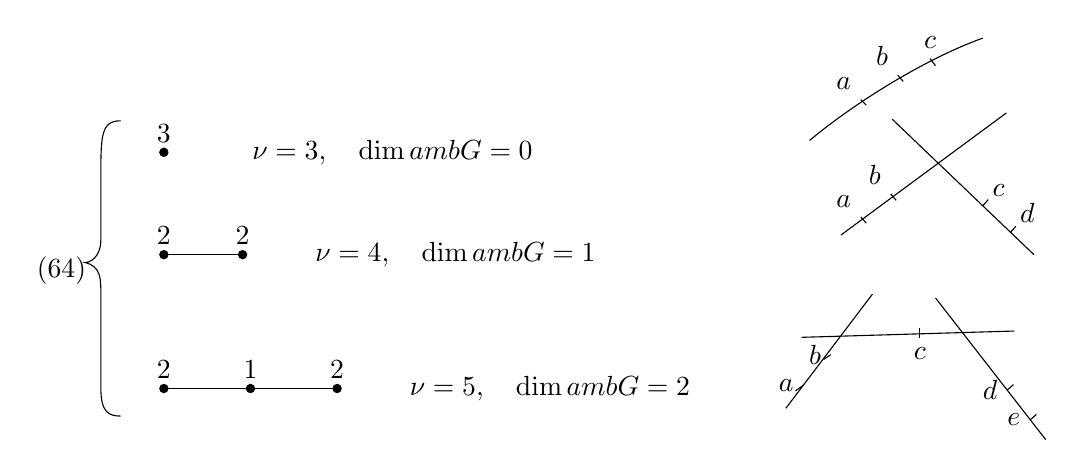
\begin{tikzpicture}[x=1cm,y=1cm]
\node at (-1.3,-1.5) {$(64)$};
\draw (-.55,.4) .. controls (-.8,.4) and (-.8,.2) .. (-.8,-.3) -- (-.8,-1.1) .. controls (-.8,-1.35) and (-.95,-1.4) .. (-1,-1.4) .. controls (-.8,-1.45) and (-.8,-1.6) .. (-.8,-1.8) -- (-.8,-3.0) .. controls (-.8,-3.3) and (-.7,-3.35) .. (-.55,-3.35);
\fill (0,0) circle (1.7pt); \node[above] at (0,0) {$3$};
\node[right] at (1,0) {$\nu=3,\quad\dim\operatorname{amb}G=0$};
\draw (0,-1.3)--(1,-1.3); \fill (0,-1.3) circle (1.7pt); \fill (1,-1.3) circle (1.7pt);\node[above] at (0,-1.3) {$2$};\node[above] at (1,-1.3) {$2$};
\node[right] at (1.8,-1.3) {$\nu=4,\quad\dim\operatorname{amb}G=1$};
\draw (0,-3)--(2.2,-3);\fill (0,-3) circle (1.7pt);\fill (1.1,-3) circle (1.7pt);\fill (2.2,-3) circle (1.7pt);
\node[above] at (0,-3) {$2$};\node[above] at (1.1,-3) {$1$};\node[above] at (2.2,-3) {$2$};\node[right] at (3,-3) {$\nu=5,\quad\dim\operatorname{amb}G=2$};
\draw (8.2,.15) .. controls (8.8,.65) and (9.7,1.2) .. (10.4,1.45);
\draw (8.85,.67)--(8.92,.60);\node[above left] at (8.85,.67) {$a$};\draw (9.32,.98)--(9.39,.90);\node[above left] at (9.32,.98) {$b$};\draw (9.73,1.19)--(9.80,1.10);\node[above] at (9.73,1.19) {$c$};
\draw (8.6,-1.05)--(10.7,.5);\draw (9.25,.42)--(11.05,-1.3);
\draw (8.85,-.82)--(8.92,-.9);\node[above left] at (8.85,-.82) {$a$};\draw (9.23,-.53)--(9.30,-.61);\node[above left] at (9.23,-.53) {$b$};\draw (10.4,-.68)--(10.47,-.60);\node[above right] at (10.4,-.68) {$c$};\draw (10.75,-1.02)--(10.82,-.94);\node[above right] at (10.75,-1.02) {$d$};
\draw (8.1,-2.35)--(10.8,-2.27);\draw (7.9,-3.25)--(9,-1.8);\draw (9.8,-1.85)--(11.2,-3.65);
\draw (8.12,-2.96)--(8.02,-3.03);\node[left] at (8.12,-2.96) {$a$};\draw (8.47,-2.57)--(8.38,-2.63);\node[left] at (8.47,-2.57) {$b$};\draw (9.6,-2.36)--(9.6,-2.23);\node[below] at (9.6,-2.36) {$c$};\draw (10.71,-3.02)--(10.79,-2.95);\node[left] at (10.71,-3.02) {$d$};\draw (11.0,-3.4)--(11.08,-3.33);\node[left] at (11,-3.4) {$e$};
\end{tikzpicture}}
\margin{52}
\scanpage{54}
\mspage{26}
b) $h_1=1$, donc $\dim\operatorname{amb}G=\nu$, on veut $0\leq\nu\leq2$. On voit que le graphe $G$ a au maximum un bout, tous les autres sommets étant donc d'ordre $3$. \deleted{\unsure{Et}} Mais un graphe \inserted{\unsure{top (compact)}} avec $h_1=1$ et n'ayant qu'un seul bout top. est homéom. à
\figure{\begin{tikzpicture}[x=1cm,y=1cm,baseline=-.1cm]
\draw (0,0) .. controls (-1.5,-.8) and (-1.3,1) .. (-.45,.7) .. controls (-.1,.65) and (0,.3) .. (0,0);\draw (0,0)--(1,0.04);\fill (0,0) circle (1.6pt);\fill (1,.04) circle (1.6pt);
\end{tikzpicture}},
et si \deleted{il n'y a pas} \inserted{$G$ n'a pas} de sommets d'ordre $2$, c'est qu'il est \inserted{isom.} au graphe \deleted{\unsure{qui}} combinatoire correspondant à la figure précédente. D'autre part, si le graphe n'a pas de bout, c'est qu'il est homéom. au cercle. Tous ses sommets sont d'ordre $2$, donc de poids marqué $1$, le nb de ces sommets \deleted{de} (il doit être au moins $1$) est \inserted{donc} $1$ \unsure{ou} $2$, ce qui donne
\figure{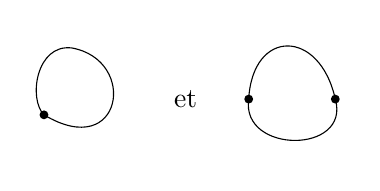
\begin{tikzpicture}[baseline=-.1cm]
\draw (0,0) .. controls (1,-.6) and (1.2,.7) .. (.35,.85) .. controls (-.1,.9) and (-.2,.2) .. (0,0);\fill (0,0) circle (1.6pt);
\node at (1.8,.2) {et};
\draw (2.6,.2) .. controls (2.65,1.1) and (3.5,1.1) .. (3.7,.2) .. controls (3.9,-.5) and (2.5,-.5) .. (2.6,.2);\fill (2.6,.2) circle (1.6pt);\fill (3.7,.2) circle (1.6pt);
\end{tikzpicture}}.
En résumé, on trouve encore trois cas :
\figure{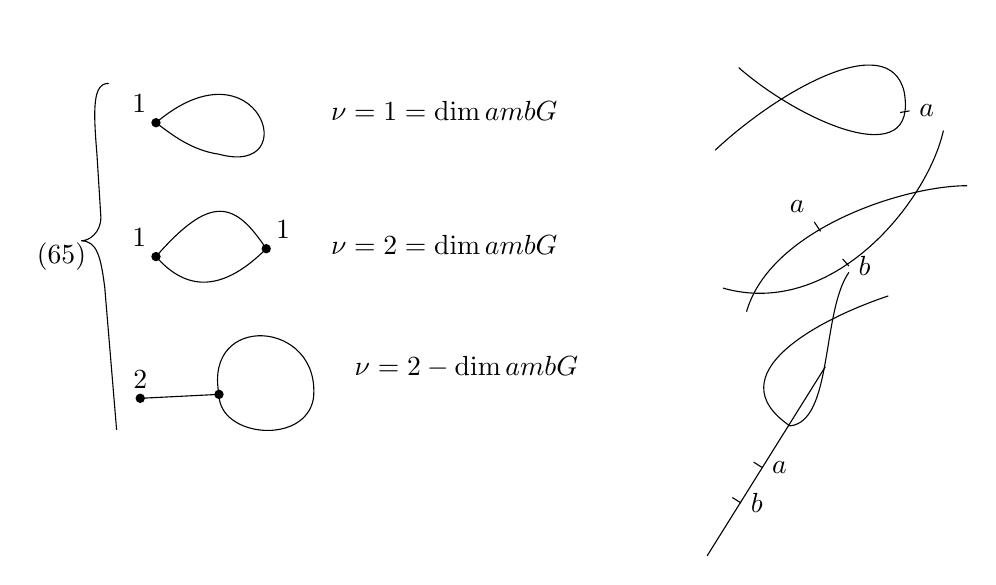
\begin{tikzpicture}[x=1cm,y=1cm]
\node at (-1.2,-1.7) {$(65)$};
\draw (-.6,.5) .. controls (-.8,.5) and (-.8,.2) .. (-.75,-.4) -- (-.7,-1.2) .. controls (-.7,-1.4) and (-.85,-1.5) .. (-.95,-1.5) .. controls (-.75,-1.5) and (-.7,-1.7) .. (-.65,-2.1) -- (-.5,-3.9);
\draw (0,0) .. controls (1.3,1.1) and (1.9,-.7) .. (.8,-.4) .. controls (.45,-.35) and (.2,-.15) .. (0,0);\fill (0,0) circle (1.7pt);\node[above left] at (0,0) {$1$};\node[right] at (2.1,.15) {$\nu=1=\dim\operatorname{amb}G$};
\draw (0,-1.7) .. controls (.7,-.9) and (1,-1) .. (1.4,-1.6) .. controls (.8,-2.2) and (.35,-2.1) .. (0,-1.7);\fill (0,-1.7) circle (1.7pt);\fill (1.4,-1.6) circle (1.7pt);\node[above left] at (0,-1.7) {$1$};\node[above right] at (1.4,-1.6) {$1$};\node[right] at (2.1,-1.55) {$\nu=2=\dim\operatorname{amb}G$};
\draw (-.2,-3.5)--(.8,-3.45);\draw (.8,-3.45) .. controls (.6,-2.4) and (2.1,-2.5) .. (2,-3.5) .. controls (1.9,-4.1) and (.8,-4) .. (.8,-3.45);\fill (-.2,-3.5) circle (1.7pt);\fill (.8,-3.45) circle (1.7pt);\node[above] at (-.2,-3.5) {$2$};\node[right] at (2.4,-3.1) {$\nu=2-\dim\operatorname{amb}G$};
\draw (7.4,.7) .. controls (8.2,0) and (9.7,-.65) .. (9.5,.4) .. controls (9.3,1.2) and (7.9,.4) .. (7.1,-.35);\draw (9.45,.13)--(9.57,.15);\node[right] at (9.57,.15) {$a$};
\draw (7.5,-2.4) .. controls (7.8,-1.35) and (9.5,-.8) .. (10.3,-.8);\draw (7.2,-2.1) .. controls (8.6,-2.5) and (9.8,-1) .. (10,-.1);\draw (8.44,-1.38)--(8.36,-1.26);\node[above left] at (8.36,-1.26) {$a$};\draw (8.72,-1.73)--(8.8,-1.82);\node[right] at (8.8,-1.82) {$b$};
\draw (7,-5.5)--(8.5,-3.1);\draw (8.05,-3.85) .. controls (7.1,-3.2) and (8.4,-2.5) .. (9.3,-2.2);\draw (8.05,-3.85) .. controls (8.6,-3.8) and (8.45,-2.4) .. (8.8,-1.9);\draw (7.7,-4.38)--(7.59,-4.31);\node[right] at (7.7,-4.38) {$a$};\draw (7.43,-4.83)--(7.32,-4.76);\node[right] at (7.43,-4.83) {$b$};
\end{tikzpicture}}
\margin{53}
\scanpage{55}
Nous allons aussi déterminer les groupes modulaires $\Gamma$ et $\Gamma^!$ correspondant à ces six cas :
\margin{MD-graphes \unsure{maximaux|minimaux} (dim mod. nulle), de dim. modulaire ambiante $\leq2$}
\figure{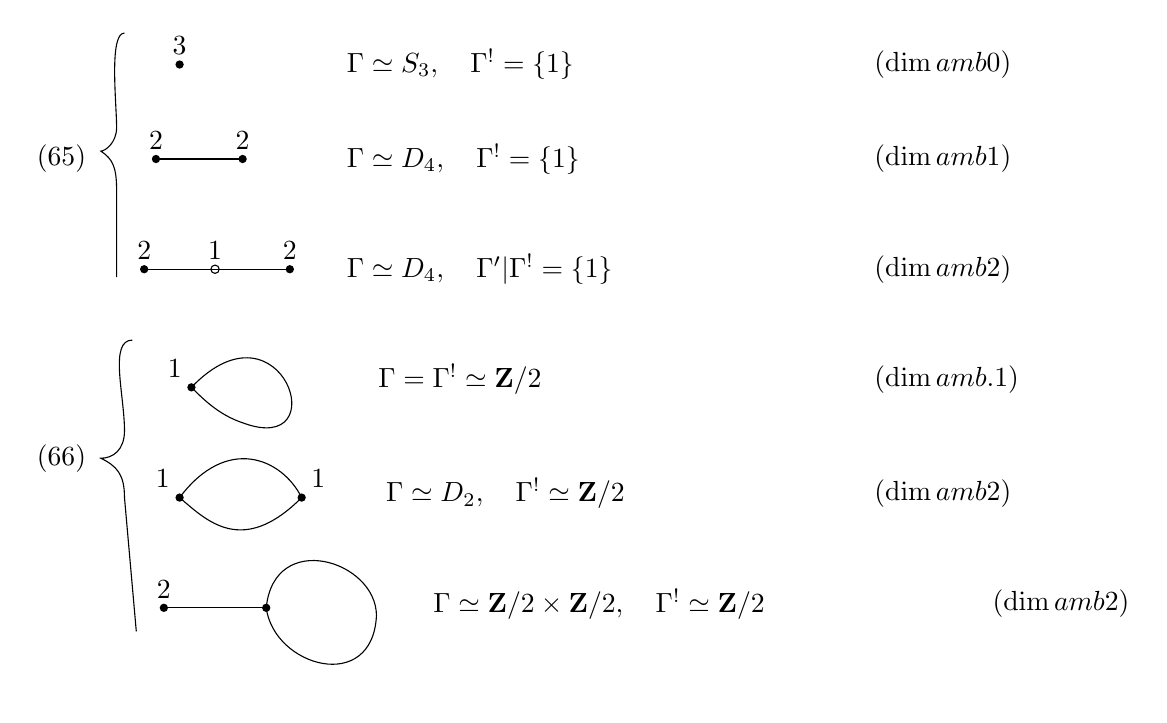
\begin{tikzpicture}[x=1cm,y=1cm]
\node at (-1.5,-1.2) {$(65)$};\draw (-.7,.4) .. controls (-.9,.4) and (-.8,-.5) .. (-.8,-.8) .. controls (-.8,-1) and (-.95,-1.1) .. (-1,-1.1) .. controls (-.85,-1.2) and (-.8,-1.3) .. (-.8,-1.6) -- (-.8,-2.7);
\fill (0,0) circle(1.5pt);\node[above] at (0,0) {$3$};\node[right] at (2,0) {$\Gamma\simeq\unsure{\mathfrak S}_3,\quad\Gamma^!=\{1\}$};\node[right] at (8.7,0) {$(\dim\operatorname{amb}0)$};
\draw (-.3,-1.2)--(.8,-1.2);\fill (-.3,-1.2) circle(1.5pt);\fill (.8,-1.2) circle(1.5pt);\node[above] at (-.3,-1.2) {$2$};\node[above] at (.8,-1.2) {$2$};\node[right] at (2,-1.2) {$\Gamma\simeq D_4,\quad\Gamma^!=\{1\}$};\node[right] at (8.7,-1.2) {$(\dim\operatorname{amb}1)$};
\draw (-.45,-2.6)--(1.4,-2.6);\fill (-.45,-2.6) circle(1.5pt);\draw (.45,-2.6) circle(1.5pt);\fill (1.4,-2.6) circle(1.5pt);\node[above] at (-.45,-2.6) {$2$};\node[above] at (.45,-2.6) {$1$};\node[above] at (1.4,-2.6) {$2$};\node[right] at (2,-2.6) {$\Gamma\simeq D_4,\quad\unsure{\Gamma'|\Gamma^!}=\{1\}$};\node[right] at (8.7,-2.6) {$(\dim\operatorname{amb}2)$};
\node at (-1.5,-5) {$(66)$};\draw (-.6,-3.5) .. controls (-.9,-3.5) and (-.7,-4.2) .. (-.7,-4.65) .. controls (-.7,-4.9) and (-.85,-5) .. (-1,-5) .. controls (-.8,-5.1) and (-.7,-5.2) .. (-.7,-5.5) -- (-.55,-7.2);
\draw (.15,-4.1) .. controls (1.3,-2.9) and (2,-5) .. (.8,-4.55) .. controls (.5,-4.45) and (.3,-4.25) .. (.15,-4.1);\fill (.15,-4.1) circle(1.5pt);\node[above left] at (.15,-4.1) {$1$};\node[right] at (2.4,-4) {$\Gamma=\Gamma^!\simeq\mathbf Z/2$};\node[right] at (8.7,-4) {$(\dim\operatorname{amb}.1)$};
\draw (0,-5.5) .. controls (.6,-4.7) and (1.3,-5) .. (1.55,-5.5) .. controls (.8,-6.25) and (.35,-5.8) .. (0,-5.5);\fill (0,-5.5) circle(1.5pt);\fill (1.55,-5.5) circle(1.5pt);\node[above left] at (0,-5.5) {$1$};\node[above right] at (1.55,-5.5) {$1$};\node[right] at (2.5,-5.45) {$\Gamma\simeq D_2,\quad\Gamma^!\simeq\mathbf Z/2$};\node[right] at (8.7,-5.45) {$(\dim\operatorname{amb}2)$};
\draw (-.2,-6.9)--(1.1,-6.9);\draw (1.1,-6.9) .. controls (1.2,-5.9) and (2.5,-6.3) .. (2.5,-7.0) .. controls (2.45,-8) and (1.2,-7.65) .. (1.1,-6.9);\fill (-.2,-6.9) circle(1.5pt);\fill (1.1,-6.9) circle(1.5pt);\node[above] at (-.2,-6.9) {$2$};\node[right] at (3.1,-6.85) {$\Gamma\simeq\mathbf Z/2\times\mathbf Z/2,\quad\Gamma^!\simeq\mathbf Z/2$};\node[right] at (10.2,-6.85) {$(\dim\operatorname{amb}2)$};
\end{tikzpicture}}
Notons que pour un \inserted{MD-}graphe $G$ de dim modulaire nulle, si $(\mathcal X,I_S)$ est une \inserted{MD-}courbe \deleted{\unsure{à}} $G$-épinglée sur une base $S$ connexe, alors le groupe des autom. de $(\mathcal X,I_S)$ (où on a oublié l'épinglage) est can. isom. à $\Gamma$, et \deleted{alors} le \deleted{$\unsure{X,I}$} sous-groupe qui induit l'identité sur $I_S$ est can. isom. à $\Gamma^!$.
\margin{54}
\scanpage{56}
\mspage{27}
Revenons au cas d'un MD-graphe général $\underline G$. Sa dimension modulaire est
\[
\text{(67)}\qquad\delta(G)=\sum_{\alpha\in S}\underbrace{\bigl(3(g_\alpha-1)+\nu_\alpha+\widetilde\mu_\alpha\bigr)}_{\delta_\alpha}.
\]
Si on veut qu'elle soit égale à $1$ ou $2$, cela signifie que l'on est dans l'un des deux cas :
\[
\left\{\begin{array}{l}
1\text{ ou }2\text{ des }\delta_\alpha\text{ sont égaux à }1,\text{ les autres sont nuls}\\
1\text{ des }\delta_\alpha\text{ est égal à }2,\text{ les autres sont nuls}
\end{array}\right.
\]
Le cas $\delta(G)=1$ correspond au cas où exactement un des $\delta_\alpha$ est $=1$, les autres étant nuls.

II) $\underline G$ \uline{de dim modulaire $1$}

Cela signifie qu'il existe un sommet $\alpha_0$ (et un seul, \deleted{de fait}) de $\underline G$ qui \deleted{soit de genre} \inserted{satisfasse la} condition
\[
\begin{aligned}
\text{(68)}\quad &(\alpha_0\text{ de genre }1,\text{ et son poids total }\nu_{\alpha_0}+\widetilde\mu_{\alpha_0}\text{ est ég. à }\unsure{1},\\
&\qquad\text{i.e. }\alpha_0\text{ est d'ordre }1,\text{ ou sommet isolé de poids marqué }1)\\
&\uline{\text{ou}}\quad(\alpha_0\text{ de genre }0,\text{ et son poids total }\nu_{\alpha_0}+\widetilde\mu_{\alpha_0}=4,\\
&\qquad\text{i.e. }(\nu_{\alpha_0},\widetilde\mu_{\alpha_0})\in\{(4,0),(3,1),(2,2),(1,3),(0,4)\}),
\end{aligned}
\]
avec en plus
\[
\begin{aligned}
\text{(69)}\quad&\text{les sommets }\alpha\ne\alpha_0\text{ sont de genre }0,\\
&\text{d'ordre }\widetilde\mu_\alpha\leq3,\text{ et pour un tel }\alpha\text{ le poids}\\
&\text{marqué }\nu_\alpha\text{ est égal à : }3-\widetilde\mu_\alpha.
\end{aligned}
\]
\deleted{On voit que la MD-structure d'un tel graphe}
\margin{55}
\scanpage{57}
\deleted{est déterminée par la structure de graphe avec un sommet particulier \unsure{par le}}

Les cas les plus simples sont les cas élémentaires (graphes \deleted{à un \unsure{pt}} \inserted{ponctuels})
\margin{MD-graphes élémentaires (sommet isolé \inserted{\unsure{i.e. de dim modulaire nulle|i.e. en dim modulaire nulle}}) de dim. modulaire $1$ \deleted{\illegible{1}} \deleted{\unsure{de dim}\ $1$}}
\figure{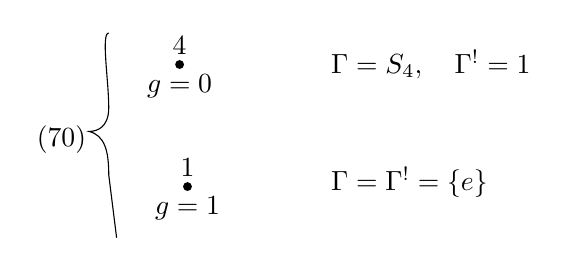
\begin{tikzpicture}[x=1cm,y=1cm]
\node at (-1.3,-.75) {$(70)$};\draw (-.7,.6) .. controls (-.8,.6) and (-.7,0) .. (-.7,-.35) .. controls (-.7,-.6) and (-.85,-.65) .. (-.95,-.65) .. controls (-.75,-.7) and (-.7,-.9) .. (-.7,-1.2) -- (-.6,-2);
\fill (.2,.2) circle(1.6pt);\node[above] at (.2,.2) {$4$};\node[below] at (.2,.2) {$g=0$};\node[right] at (2,.2) {$\Gamma=\unsure{\mathfrak S}_4,\quad\Gamma^!=1$};
\fill (.3,-1.35) circle(1.6pt);\node[above] at (.3,-1.35) {$1$};\node[below] at (.3,-1.35) {$g=1$};\node[right] at (2,-1.3) {$\Gamma=\Gamma^!=\{e\}$};
\end{tikzpicture}}
Les autres cas sont ceux des \inserted{MD-}graphes ``\uline{rationnels}'' (tous les $g_\alpha$ nuls) tels que tous les $\widehat\nu_\alpha$ soient égaux à trois (donc les sommets d'ordre $1\leq\widetilde\mu_\alpha\leq3$) \deleted{\unsure{et un}} \inserted{sauf l'}un d'eux, qui est égal à $4$ (donc $1\leq\widetilde\mu_{\alpha_0}\leq4$), ou bien des \inserted{MD-}graphes qui ont tous leurs sommets sauf un rationnels et $\widehat\nu_\alpha=3$, \deleted{(donc} sauf un \inserted{$\alpha_0$} qui est un sommet-bout ($\widetilde\mu_\alpha=1$) et de genre $1$, $\nu_{\alpha_0}=0$ --- donc ici tous les sommets sont d'ordre $1\leq\widetilde\mu_\alpha\leq3$, et les $\nu_\alpha$ \inserted{pour $\alpha\ne\alpha_0$} sont égaux à $3-\widetilde\mu_\alpha$, \deleted{pour $\alpha\ne$} et $\nu_{\alpha_0}=0$.

Dans l'un et l'autre cas \inserted{($g_{\alpha_0}=0$, $g_{\alpha_0}=1$)} on aura un iso can. de multiplicités
\[
\text{(71)}\qquad\widehat M_G\simeq\widehat M_{g_{\alpha_0},\widehat I_{\alpha_0}}
\]
\margin{avec $\widehat I_{\alpha_0}=I_{\alpha_0}+\widetilde A_{\alpha_0}$ (de cardinal $4$ ou $1$ suivant que $g_{\alpha_0}=0$ ou $g_{\alpha_0}=1$)}
\margin{56}
\scanpage{58}
\mspage{28}
\deleted{\unsure{(71)}} et. l'action de $\Gamma_{\underline G}=\Gamma$ sur $\widehat M_G\simeq\widehat M_{g_{\alpha_0},\widehat I_{\alpha_0}}$ est triviale si $g_{\alpha_0}=1$, et elle se fait à travers
\diagram{\begin{tikzcd}[ampersand replacement=\&]
\text{(72)}\quad\Gamma_{\underline G}\arrow[r]\&\unsure{\mathfrak S}_{\widehat I_{\alpha_0}}\quad(\simeq\unsure{\mathfrak S}_4)
\end{tikzcd}}
dans le cas où $g_{\alpha_0}=0$. L'image de $\Gamma_{\underline G}$ dans $\mathfrak S_4$ doit pouvoir être n'importe quel sous-groupe de $\mathfrak S_4$, sauf erreur. Explicitons déjà quels sont les cas où la dim. ambiante est $\leq2$. Le cas de la dim. ambiante $1$ \inserted{i.e. où la codim modulaire \inserted{$s_1$} de $\underline G$ est $0$,} est évidemment celui donné par (70), où $G$ est réduit à un sommet isolé.

Considérons donc le cas de la dim mod ambiante $2$, i.e. codim modulaire $1$, i.e. \uline{une} arête. On trouve soit
\figure{\begin{tikzpicture}[baseline=-.1cm]\draw (0,0) .. controls (.8,.9) and (1.4,-.4) .. (.55,-.3) .. controls (.2,-.2) and (.1,-.1) .. (0,0);\fill (0,0) circle(1.5pt);\node at (1.7,0) {, soit};\draw (2.6,0)--(3.6,0);\draw (2.6,0) circle(1.5pt);\fill (3.6,0) circle(1.5pt);\end{tikzpicture}}.
\inserted{On trouve les trois cas de dim modulaire} \deleted{Dans le cas $g_{\alpha_0}=0$ tous les sommets sauf $1$ sont d'ordre $\unsure{2}$} ambiante $2$, dim. modulaire $1$
\margin{MD-graphes de dim mod $1$, dim. modulaire ambiante $2$.}
\figure{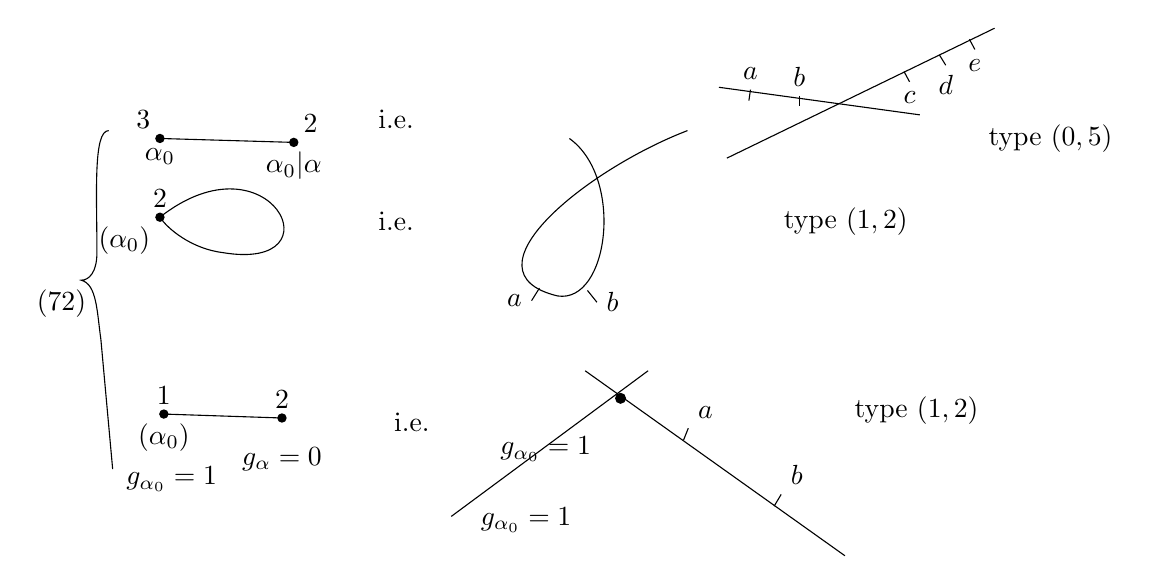
\begin{tikzpicture}[x=1cm,y=1cm]
\node at (-1.25,-1.7) {$(72)$};\draw (-.65,.5) .. controls (-.85,.5) and (-.8,-.3) .. (-.8,-1.05) .. controls (-.8,-1.3) and (-.9,-1.4) .. (-1,-1.4) .. controls (-.8,-1.45) and (-.8,-1.8) .. (-.75,-2.15) -- (-.6,-3.8);
\draw (0,.4)--(1.7,.35);\fill (0,.4) circle(1.7pt);\fill (1.7,.35) circle(1.7pt);\node[above left] at (0,.4) {$3$};\node[below] at (0,.4) {$\alpha_0$};\node[above right] at (1.7,.35) {$2$};\node[below] at (1.7,.35) {$\unsure{\alpha_0|\alpha}$};\node at (3,.65) {i.e.};
\draw (0,-.6) .. controls (1.4,.5) and (2.3,-1.3) .. (.8,-1.05) .. controls (.4,-1) and (.1,-.75) .. (0,-.6);\fill (0,-.6) circle(1.7pt);\node[above] at (0,-.6) {$2$};\node[below left] at (0,-.6) {$(\alpha_0)$};\node at (3,-.65) {i.e.};
\draw (.05,-3.1)--(1.55,-3.15);\fill (.05,-3.1) circle(1.7pt);\fill (1.55,-3.15) circle(1.7pt);\node[above] at (.05,-3.1) {$\deleted{\unsure{1}}$};\node[above] at (1.55,-3.15) {$2$};\node[below] at (.05,-3.1) {$(\alpha_0)$};\node[below] at (.15,-3.65) {$g_{\alpha_0}=1$};\node[below] at (1.55,-3.4) {$g_\alpha=0$};\node at (3.2,-3.2) {i.e.};
\draw (7.1,1.05)--(9.65,.7);\draw (7.2,.15)--(10.6,1.8);\draw (7.5,1.02)--(7.48,.88);\node[above] at (7.5,1.02) {$a$};\draw (8.12,.94)--(8.12,.81);\node[above] at (8.12,.94) {$b$};\draw (9.45,1.25)--(9.52,1.12);\node[below] at (9.52,1.12) {$c$};\draw (9.9,1.46)--(9.98,1.33);\node[below] at (9.98,1.33) {$d$};\draw (10.28,1.66)--(10.35,1.53);\node[below] at (10.35,1.53) {$e$};\node[right] at (10.4,.4) {type $(0,5)$};
\draw (5.2,.4) .. controls (5.9,-.1) and (5.7,-1.7) .. (5.05,-1.6) .. controls (3.8,-1.3) and (5.4,0) .. (6.7,.5);\draw (4.82,-1.5)--(4.72,-1.66);\node[left] at (4.72,-1.66) {$a$};\draw (5.43,-1.53)--(5.55,-1.68);\node[right] at (5.55,-1.68) {$b$};\node[right] at (7.8,-.65) {type $(1,2)$};
\draw (3.7,-4.4)--(6.2,-2.55);\draw (5.4,-2.55)--(8.7,-4.9);\fill (5.85,-2.9) circle(2pt);\node at (4.9,-3.55) {$\deleted{\unsure{g_{\alpha_0}}=1}$};\node at (4.65,-4.45) {$g_{\alpha_0}=1$};\draw (6.65,-3.43)--(6.71,-3.28);\node[above right] at (6.71,-3.28) {$a$};\draw (7.8,-4.27)--(7.89,-4.12);\node[above right] at (7.89,-4.12) {$b$};\node[right] at (8.7,-3.05) {type $(1,2)$};
\end{tikzpicture}}
(NB les sommets, ou branches des courbes, dont le genre \inserted{ou poids marqué} n'est pas marqué en dessous, sont de genre \inserted{ou poids marqué} zéro; les poids marqués sont indiqués sur le graphe \unsure{au|en} dessus des sommets)
\margin{57}
\scanpage{59}
Les groupes d'automorphismes de ces MD-graphes sont
\figure{\begin{tikzpicture}[x=1cm,y=1cm]
\node at (-1.25,-1) {$(73)$};\draw (-.7,.6) .. controls (-.9,.6) and (-.8,0) .. (-.8,-.5) .. controls (-.8,-.7) and (-.9,-.8) .. (-1,-.8) .. controls (-.8,-.9) and (-.8,-1.1) .. (-.75,-1.5) -- (-.65,-2.4);
\draw (0,.35)--(1.5,.35);\fill (0,.35) circle(1.5pt);\fill (1.5,.35) circle(1.5pt);\node[above] at (0,.35) {$3$};\node[above] at (1.5,.35) {$\unsure{3|2}$};\node[below] at (0,.35) {$\alpha_0$};\node[right] at (2.4,.4) {$\Gamma=\unsure{\mathfrak S}_3\times\mathfrak S_2,\quad\Gamma^!=1,\quad\operatorname{Im}(\Gamma\to\mathfrak S_4)\simeq\mathfrak S_3$};
\draw (0,-.85) .. controls (2,.3) and (2.25,-1.3) .. (1,-.95) -- (0,-.85);\fill (0,-.85) circle(1.5pt);\node[above] at (0,-.85) {$2$};\node[below] at (0,-.85) {$(\alpha_0)$};\node[right] at (2.4,-.8) {$\Gamma\simeq\mathfrak S_2\times\mathfrak S_2,\quad\Gamma^!\simeq\mathfrak S_2,\quad\operatorname{Im}(\Gamma\to\mathfrak S_4)\simeq\underset{\substack{\Vert\\\mathfrak S_2\times\mathfrak S_2}}\Gamma$};
\draw (0,-2.2)--(1.7,-2.2);\fill (0,-2.2) circle(1.5pt);\fill (1.7,-2.2) circle(1.5pt);\node[above] at (1.7,-2.2) {$2$};\node[below] at (0,-2.2) {$g_{\alpha_0}=1$};\node[right] at (2.4,-2.1) {$\Gamma\simeq\mathfrak S_2,\quad\Gamma^!\simeq1\quad\deleted{\unsure{\operatorname{Im}(\Gamma\to\mathfrak S_4)=1}}$};
\end{tikzpicture}}

III) \uline{Dim. modulaire $2$}

Correspond par (67) aux deux cas suivants :

$1^\circ)$ Tous les $\alpha\in S$ sauf un seul \inserted{$\alpha_0$} sont de genre $0$, et de poids total $3$ (i.e. d'ordre \inserted{$\widetilde\mu_\alpha$} $\leq3$, et de poids marqué $3-\widetilde\mu_\alpha$), et $(\unsure{\alpha_0|g_{\alpha_0}},\widehat\nu_{\alpha_0})$ est d'un des deux types $(0,5)$, $(1,2)$ \deleted{$\unsure{(2,0)}$}, i.e. $\alpha_0$ est de genre $0$, d'ordre \inserted{$\widetilde\mu_{\alpha_0}$} $\leq5$ et de poids marqué $5-\widetilde\mu_{\alpha_0}$, \uline{ou} $\alpha_0$ de genre $1$, d'ordre \deleted{$\unsure{\leq2}$} \inserted{$\widetilde\mu_{\alpha_0}\in\{1,2\}$} et de poids marqué $2-\widetilde\mu_{\alpha_0}\in\{1,0\}$.
\margin{donc deux cas en réalité}

$2^\circ)$ Tous les $\unsure{\alpha=S|\alpha\in S}$ sauf deux exactement $\alpha_0$ et $\alpha_1$, sont de genre $0$, \inserted{et} de poids total $3$ (i.e. d'ordre $1\leq\widetilde\mu_\alpha\leq3$, et de poids marqué égal à $3-\widetilde\mu_\alpha$), $\alpha_0$ et $\alpha_1$ sont chacun \deleted{soit} de type $(\unsure{\alpha_i|g_i},\unsure{\widehat\mu_i|\widehat\nu_i})$ égal soit $(0,4)$, soit à $(1,1)$.
\margin{Cela fait donc trois cas, suivant que les deux types de dim mod $1$ qui interviennent sont tous deux $(0,4)$, ou l'un $(0,4)$, l'autre $(1,1)$, ou tous deux $(1,1)$.}

La \deleted{\unsure{schéma|variété}} \inserted{mult.} modulaire $\widehat M_G$ est alors isomorphe, suivant les cas, à l'une des suivantes :
\margin{58}
\scanpage{60}
\mspage{29}
\margin{\unsure{multiplicités} modulaires de dim $2$ $(\widehat M_G)$}
\[
(74)\quad\left\{\begin{array}{ll}
\widehat M^!_{0,5}&\Gamma\text{ opère via }\Gamma\longrightarrow\mathfrak S_{\widehat I_{\alpha_0}}\ (\simeq\mathfrak S_5)\\
\widehat M^!_{1,2}&\Gamma\text{ \unsure{---} }\quad\Gamma\longrightarrow\mathfrak S_{\widehat I_{\alpha_0}}\simeq\mathbf Z/2\mathbf Z\\
\widehat M^!_{0,4}\times\widehat M^!_{0,4}&\Gamma\text{ --- }\quad\Gamma\longrightarrow\deleted{\unsure{\mathfrak S_{\alpha_0,\alpha_1}}}\mathfrak S_{\deleted{\unsure{\widehat I}}(\widehat I_{\alpha_0}\amalg\widehat I_{\alpha_1})}\simeq\mathfrak S_8\\
\widehat M^!_{0,4}\times\widehat M^!_{1,1}&\Gamma\text{ --- }\quad\Gamma\longrightarrow\mathfrak S^{\unsure{\deleted{*}|*}}_{\widehat I_{\alpha_0}}\simeq\mathfrak S_4\\
\widehat M^!_{1,1}\times\widehat M^!_{1,1}&\Gamma\text{ opère trivialement.}
\end{array}\right.
\]

\uline{NB} \deleted{\unsure{à}} Dans le cas $3^\circ$ de $\widehat M_{0,4}\times\widehat M_{0,4}$, $\Gamma$ \deleted{opère}\inserted{s'envoie} dans $\mathfrak S_8$ par l'intermédiaire de
\[
\Gamma\longrightarrow\underbrace{\mathbf Z/2\mathbin{\cdot}(\mathfrak S_4\times\mathfrak S_4)}_{\text{prod. }\frac12\text{ direct}}
\]

On peut considérer que par rapport aux schémas modulaires \inserted{$\widehat M_G$} de dim $1$, \deleted{\unsure{qui sont}}\inserted{ils sont deux :}
\margin{(cas élémentaires!)}
\[
(75)\quad\left\{\begin{array}{ll}
\widehat M^!_{0,4}&\Gamma\text{ opère via }\Gamma\longrightarrow\mathfrak S_{\widehat I_{\alpha_0}}\simeq\mathfrak S_4\\
\widehat M^!_{1,1}&\Gamma\text{ opère trivialt},
\end{array}\right.
\]
les ``cas nouveaux'' de (74) sont $\widehat M^!_{0,5}$ et $\widehat M^!_{1,2}$.

Cela fait en tous essentiellement quatre cas ``élémentaires'' à étudier à fond, pour le cas des dim. modulaires $\leq2$. J'ai l'impression qu'une compréhension plus ou moins complète de la structure des $\pi_1$ \inserted{discrets (i.e. dans le contexte analytique)} impliqués dans ces cas, donnerait la clef pour une compréhension complète dans le cas général.
\margin{59}
\scanpage{61}
Partant des MD-graphes ``élémentaires'' correspondants, je voudrais expliciter dans les quatre cas la structure \inserted{de spécialisation entre} des strates des $\widehat M_{g,\nu}$ et $\widehat M^!_{g,\nu}$.

8) \uline{Structure de spécialisation des strates en dim modulaire $\leq2$.}

$1^\circ)$ \uline{Cas de} $\widehat M^!_{0,4}$ \uline{et} $\widehat M_{0,4}$

Commençons par $\widehat M^!_{0,4}$.
\[
(76)\quad\left\{\diagram{\begin{array}{c|c}
\text{Codim }0&\text{Codim }1\\\hline
\figure{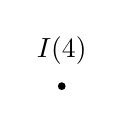
\begin{tikzpicture}[baseline=-2pt]\fill (0,0) circle (1.4pt);\node[above] at (0,.15) {$I(4)$};\end{tikzpicture}}\quad\xrightarrow{3}&
\figure{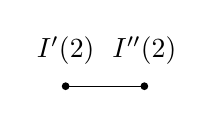
\begin{tikzpicture}[baseline=-2pt]\draw (0,0)--(1,0);\fill (0,0) circle (1.4pt);\fill (1,0) circle (1.4pt);\node[above] at (0,.15) {$I'(2)$};\node[above] at (1,.15) {$I''(2)$};\end{tikzpicture}}
\end{array}}\right.
\]
Le diagramme signifie que l'ens. marqué $I$ de cardinal $4$, \inserted{\unsure{se partageant}} suivant l'une quelc. des trois partitions de $I$ en $I'$ et $I''$ de cardinal $2$ chacun, donne $3$ spécialisations différentes de la strate maxima --- cela correspond bien sûr aux trois pts à l'infini de $U_{0,3}$

on aura
\[
(77)\qquad \widehat M^!_{0,4}\simeq\mathbf P^1_{\mathbf Z},\quad M^!_{0,4}\simeq(U_{0,3})_{\mathbf Z}=\mathbf P^1_{\mathbf Z}\smallsetminus\{0,1,\infty\}
\]
Pour bien faire, il faudrait aussi expliciter
\margin{60}
\scanpage{62}
\mspage{30}
la courbe modulaire $\widehat X^!_{0,4}$ sur $\widehat M^!_{0,4}$, avec ses quatre sections $s_0,s_1,s_\infty,s_\lambda$ (ou $t_1,t_2,t_3,t_4$) et avec l'opération de $\mathfrak S_4$ \deleted{dessus} sur $\widehat X^!_{0,4}\longrightarrow\widehat M^!_{0,4}$, échangeant ces quatre sections entre elles. Je vais pas le faire ici --- cela donnera du $=$ coup les \deleted{schémas}\inserted{multiplicités} modulaires $\widehat M_{0,4}$ et $\widehat X_{0,4}$. Pour $\widehat M_{0,4}$, il y a lieu de remplacer le diagramme (76) par un diagramme purement numérique
\[
(78)\quad\left\{\diagram{\begin{array}{c|c}
\text{codim }0&\text{codim }1\\\hline
\figure{\begin{tikzpicture}[baseline=-2pt]\fill (0,0) circle (1.4pt);\node[above] at (0,.15) {$4$};\end{tikzpicture}}\quad\xrightarrow{1}&
\figure{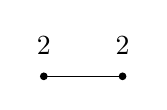
\begin{tikzpicture}[baseline=-2pt]\draw (0,0)--(1,0);\fill (0,0) circle (1.4pt);\fill (1,0) circle (1.4pt);\node[above] at (0,.15) {$2$};\node[above] at (1,.15) {$2$};\end{tikzpicture}}
\end{array}}\right.
\]
il n'y a plus qu'un seul pt à l'infini, correspondant aux trois pts à l'infini de $\widehat M^!_{0,4}$, permutés transitivement entre eux par $\mathfrak S_4$.

Caractéristiques d'EP fractionnaires. On trouve
\[
\begin{aligned}
\chi_!(M^{!\,\mathrm{an}}_{0,4})&=\chi_!(U^{\mathrm{an}}_{0,3})=2-2\underset{\substack{\Vert\\0}}{g}-\underset{\substack{\Vert\\3}}{\nu}=-1\\
\chi_!(\widehat M^{!\,\mathrm{an}}_{0,4})&=\chi_!(\mathbf P^{1\,\mathrm{an}})=2\\
\chi_!(\overset{\deleted{\unsure{\widehat{\phantom M}\,!}}}{M}{}^{\mathrm{an}}_{0,4})&=\chi_!(\unsure{U|\mathbf P}^{\mathrm{an}}_{0,3},\mathfrak S_4)\\
&=\chi_!\bigl(U^{\mathrm{an}}_{0,3}\smallsetminus\{\unsure{-\bar j},-j\}\smallsetminus\{\tfrac12,2,-1\},\mathfrak S_4\bigr)\\
&\qquad+\chi_!(\{\unsure{-\bar j},-j\},\mathfrak S_4)+\chi_!(\{\tfrac12,2,-1\},\mathfrak S_4)\\
&=-1+\frac13+\frac12=-\frac1{\unsure{24|6}}
\end{aligned}
\]
\margin{\uline{NB} On peut écrire directement $\chi_!(U^{\mathrm{an}}_{0,3}):[\mathfrak S_4]=-\frac1{24}$}
\margin{61}
\scanpage{63}
\[
\chi_!(\widehat M^{\mathrm{an}}_{0,4})=\underbrace{\chi_!(U^{\mathrm{an}}_{0,3},\mathfrak S_4)}_{-1/24}+\underbrace{\chi_!(\{0,1,\infty\},\mathfrak S_4)}_{1/8}=\frac1{12}.
\]
De façon plus fine, dans un ``groupe de Grothendieck'' convenable, on aura
\margin{valable au dessus de $\mathbf Z[\frac16]$ --- \unsure{je me dispense|pour dispenser} de faire le calcul plus fin au dessus de $\operatorname{Spec}\mathbf Z\ldots$}
\[
79\quad\left\{\begin{aligned}
[M^!_{0,4}]&=[U_{\unsure{0,4|0,3}}]=\underbrace{T(1)}_{\substack{\text{``Tate''}\simeq[\unsure{\mathbf E^1|\mathbf A^1}]\\(\text{d'augmentation }1)}}-2\\
[M_{0,4}]&=\deleted{\unsure{\tfrac1{24}(T(1)-2)}}\frac14(T(1)-2)+\frac1{12}+\frac18=\frac14(T(1)-1)-\frac1{24}\\
[\widehat M_{0,4}]&=[M_{0,4}]+\frac18=\deleted{\unsure{\tfrac1{24}(T(1)+1)}}=\frac14(T(1)-1)+\frac1{12}.
\end{aligned}\right.
\]
Ces trois quantités sont d'augmentation égale respt : $-1,-1/24,1/12$.

$2^\circ)$ \uline{Cas de} $\widehat M_{1,1}$.
\[
(77)\qquad\diagram{\begin{array}{c|c}
\text{codim }0&\text{codim }1\\\hline
\figure{\begin{tikzpicture}[baseline=-2pt]\fill (0,0) circle (1.4pt);\node[above] at (0,.15) {$1$};\node[below] at (0,-.12) {$\underline1$};\end{tikzpicture}}\quad\xrightarrow{1}&
\figure{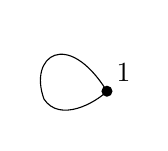
\begin{tikzpicture}[baseline=-2pt]\draw (0,0)..controls(-.5,.8)and(-1,.45)..(-.8,-.1)..controls(-.6,-.4)and(-.15,-.15)..(0,0);\fill (0,0) circle (2pt);\node[above right] at (0,0) {$1$};\end{tikzpicture}}
\end{array}}
\]
Il y a exactement un point à l'infini.

On a un morphisme (\uline{au dessus de} $\mathbf Z[\frac12]$)
\[
(78)\qquad \widehat M_{1,1}\longrightarrow\widehat M'_{\unsure{1,4|0,4}}\overset{\mathrm{déf}}=(\widehat M^!_{\unsure{1,4|0,4}},\mathfrak S_3)
\]
qui fait de $\widehat M_{1,1}$ une gerbe (de groupe constant $\{\pm1\}$) au dessus de $\widehat M'_{\unsure{1,4|0,4}}$ (en ca. $\neq2$) d'où
\[
[M_{1,1}]=\frac12[U_{0,3},\mathfrak S_3]=2[M_{0,4}]\deleted{\unsure{=\tfrac1{12}[\mathbf E^1]-\tfrac14}}\inserted{\unsure{T(1)}}
\]
\margin{62}
\scanpage{64}
\mspage{31}
d'où, au moins au dessus de $\mathbf Z[\frac12]$
\[
(79)\quad\left\{\begin{aligned}
[M_{1,1}]&=\deleted{\unsure{\tfrac1{12}(T(1)-2)}}\frac12(T(1)-1)-\frac1{12}\\
[\widehat M_{1,1}]&=[M_{1,1}]+\underset{\substack{\Vert\\1/2}}{[\widehat M^\infty_{1,1}]}=\deleted{\unsure{\tfrac{T(1)}{12}+\tfrac13}}\frac12(T(1)-1)+\frac5{12}
\end{aligned}\right.
\]
Voici un autre calcul de $[M_{1,1}]$. On considère le morphisme modulaire
\[
M_{1,1}\longrightarrow\mathbf E^1
\]
\deleted{et} en découpant $\mathbf E^1$ suivant les deux sections $S_0$ (correspondant à la courbe elliptique harmonique de groupe d'automs $\mathbf Z/4\mathbf Z$) et $S_1$ \deleted{\unsure{$\simeq\mathbf Z$}} (courbe ell. \unsure{bonne} \unsure{avec un bon} gr. d'automs $\mathbf Z/6\mathbf Z$), qui ne se coupent qu'en les pts $2$ et $3$, qui correspondent (sauf erreur) à des groupes d'automs d'ordre $24$, et $12$. On a donc une partition
\[
\mathbf E^1=\deleted{\unsure{E}}U\amalg S'_0\amalg S'_1\cup a_2\cup a_3
\]
où \deleted{\unsure{$a_1,a_0$}}
\[
\left\{\begin{aligned}
U&=\mathbf E^1\smallsetminus(S_0\cup S_1)\\
\{\underset{\substack{|\\\text{car }2}}{a_2},\underset{\substack{|\\\text{car }3}}{a_3}\}&=S_0\cap S_1\\
S'_0&=S_0\smallsetminus\{a_2,a_3\},\quad S'_1=S_1\smallsetminus\{a_2,a_3\}
\end{aligned}\right.
\]
On trouve donc
\margin{63}
\scanpage{65}
\[
M_{1,1}=\frac12[U]+\frac14[S'_0]+\frac16[S'_1]+\frac1{24}[a_2]+\frac1{12}[a_3]
\]
et on a
\[
\begin{aligned}
[U]&=[\mathbf E^1]-[S_0]-[S_1]+[a_2]+[a_3]\\
&=T(1)-2+\zeta_2+\zeta_3
\end{aligned}
\]
où de façon générale on pose, pour un nb premier $p$
\[
\unsure{\zeta_p|\xi_p}=[\operatorname{Spec}\mathbf Z/p\mathbf Z]=i_{p!}(1)
\]
où
\[
i_{p!}:K_!(\mathbf Z_p)\longrightarrow K_!(\mathbf Z).
\]
De $=$
\[
\begin{aligned}
[S'_0]&=[S_0]-[a_2]-[a_3]=1-\zeta_2-\zeta_3\\
[S'_1]&=[S_1]-[a_2]-[a_3]=1-\zeta_2-\zeta_3
\end{aligned}
\]
d'où
\[
\begin{aligned}
[M_{1,1}]&=\frac12(T(1)-2+\zeta_2\unsure{+|-}\zeta_3)+\overbrace{\left(\frac14\deleted{\unsure{+}}+\frac16\right)}^{5/12}(1-\zeta_2-\zeta_3)\\
&\qquad+\frac1{24}\zeta_2+\frac1{12}\zeta_3\\
&=\frac12T(1)-7/12\deleted{\unsure{\zeta}}+\frac18\zeta_2+\frac16\zeta_3\\
&=\frac12(T(1)-1)-\frac1{12}+\frac18\zeta_2+\frac16\zeta_3,
\end{aligned}
\]
donc
\[
(80)\quad\left\{\begin{aligned}
[M_{1,1}]&=\frac12(T(1)-1)-\frac1{12}+\frac18\zeta_2+\frac16\zeta_3\\
[\widehat M_{1,1}]&=[M_{1,1}]+\frac12=\frac12T(1)-\frac1{12}+\frac18\zeta_2+\frac16\zeta_3
\end{aligned}\right.
\]
\margin{64}
\scanpage{66}
\mspage{32}
$3^\circ)$ \uline{Cas de} $\widehat M^!_{0,5}$, ou $\widehat M_{0,I}$
\[
(81)\quad\diagram{\begin{array}{c|c|c}
\text{codim }0&\text{codim }1&\text{codim }2\\\hline
\figure{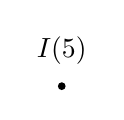
\begin{tikzpicture}[baseline=-2pt]\fill (0,0) circle (1.4pt);\node[above] at (0,.15) {$I(5)$};\end{tikzpicture}}\xrightarrow{(10)}&
\figure{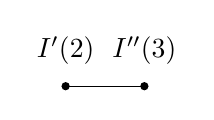
\begin{tikzpicture}[baseline=-2pt]\draw (0,0)--(1,0);\fill (0,0) circle (1.5pt);\fill (1,0) circle (1.5pt);\node[above] at (0,.15) {$I'(2)$};\node[above] at (1,.15) {$I''(3)$};\end{tikzpicture}}\xrightarrow{(3)}&
\figure{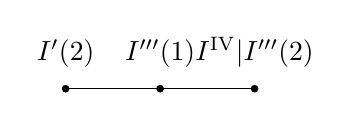
\begin{tikzpicture}[baseline=-2pt]\draw (0,0)--(1.2,0)--(2.4,0);\foreach \x in {0,1.2,2.4}{\fill (\x,0) circle (1.4pt);}\node[above] at (0,.15) {$I'(2)$};\node[above] at (1.2,.15) {$I'''(1)$};\node[above] at (2.4,.15) {$\unsure{I^{\mathrm{IV}}|I'''}(2)$};\end{tikzpicture}}
\end{array}}
\]
Dans $\widehat M^!_{0,5}$ il y a dix ``diviseurs à l'infini'' \inserted{$(I'(2),I'')$}, dont chacun est un $\widehat M^!_{0,4}$ \deleted{\unsure{$\simeq\mathbf P$}}, \deleted{\unsure{$\mathbf P^1_{0,3}\mathfrak S_3$}} \inserted{(plus précisément, un $\widehat M_{0,I''(3)\amalg(*)}\simeq(\mathbf P^1_{I''})_{\mathbf Z}$)} (ayant comme on avait vu, et \unsure{avait|aurait}) trois points à l'infini --- les pts à l'infini sont en nb total $\frac{30}{2}=15$, correspondant aux partitions de $I(5)$ de type $(2,2,1)$, alors que les diviseurs à l'infini correspondent aux parties \inserted{$I'$} de $I$ de cardinal $2$. Deux tels diviseurs, correspondant à des parties $I',I''\in\mathfrak P_2(I)$, se rencontrent sss \deleted{elles} on a $I'\cap I''=\varnothing$, i.e. si $I',I''$ et $I\smallsetminus(I'\cup I'')$ forment justement une partition de $I$ de type $(2,2,1)$.
\margin{$\mathbf P^1_{I''}\overset{\mathrm{déf}}=\unsure{\mathbf P^1_{\mathbf Z}\wedge_{\mathfrak S_3}\widetilde{I''}}$}

D'après l'étude combinatoire de l'\unsure{icosaèdre}, choisissant une orientation de $I$ --- ce qui détermine un \unsure{icosaèdre} orienté, ou encore un icos. graphe) les $10$ diviseurs à l'infini de $\widehat M_{0,I}$, i.e. les \inserted{$10$} éléments de $\mathfrak P_2(I)$, \deleted{\unsure{en ordre}} \inserted{ou (par} \deleted{\unsure{correspon-}}
\margin{65}
\scanpage{67}
passage aux complémentaires) les dix ``triangles'' de $I$, correspondent aux dix faces de l'icosaèdre gauche ($\simeq$ paires de faces opposées de l'icos. ordinaire), tandis que les $15$ partitions de type $(2,2,1)$ de $I$, qu'on peut interpréter comme les structures carrées sur quatre parmi les $5$ pts de $I$
\figure{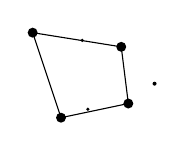
\begin{tikzpicture}[scale=.9]\draw (0,1.1)--(1.25,.9)--(1.35,.1)--(.4,-.1)--cycle;\foreach \p in {(0,1.1),(1.25,.9),(1.35,.1),(.4,-.1)}{\fill \p circle (2pt);}\fill (.7,.99) circle (.7pt);\fill (.78,.02) circle (.7pt);\fill (1.72,.38) circle (.8pt);\end{tikzpicture}}
(en associant à un tel carré les deux paires de sommets diagonalement opposés) correspondent aux $15$ arêtes dudit icosaèdre gauche.
\margin{NB on associe à un côté $a$ le jeu des ``couleurs'' des $4$ autres côtés des faces adjacentes, groupées \deleted{\unsure{deux}} en deux paires \unsure{des deux faces}.
\figure{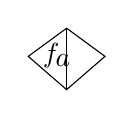
\begin{tikzpicture}[scale=.65]\draw (0,0)--(.75,.55)--(1.5,0)--(.75,-.65)--cycle;\draw (.75,.55)--(.75,-.65);\node at (.45,.02) {$f$};\node at (.68,-.08) {$a$};\end{tikzpicture}}}
Un côté \inserted{$a$} est contenu \deleted{dans}\inserted{(incident)} à une face \inserted{$f$} de l'icosaèdre, sss le ``triangle'' $\subset I$ correspondant à $f$ a comme intersection avec le carré correspondant à $a$, \deleted{deux}\inserted{l'un des} \deleted{\unsure{côt}} $2$ sommets \deleted{consécutifs}\inserted{opposés} du carré, \deleted{On voit donc.}\inserted{i.e. ssi le complémentaire du triangle est formé de l'une des deux paires définissant le carré.}
\inserted{Donc on voit que} la relation d'incidence des diviseurs à \unsure{sommets} de la structure $\widehat M_{0,I}$, correspond à celle des faces et arêtes de l'icosaèdre gauche, ou par dualité, à celle des \deleted{arêtes}\inserted{sommets} et des \deleted{faces}\inserted{arêtes} du dodécaèdre.

On a donc trouvé :
\margin{66}
\scanpage{68}
\mspage{33}
\uline{Proposition} Le diviseur à l'infini \inserted{$M^\infty_{0,I}$} de $\widehat M_{0,I}$ est une courbe \unsure{stable|semi-stable} \inserted{déployée} sur $\operatorname{Spec}\mathbf Z$, dont le graphe est isomorphe au \deleted{celui du} $1$-squelette du dodécaèdre gauche défini par $I$ (muni d'une orientation convenable).
\margin{\uline{NB} $\widehat M_{0,I}\longrightarrow$ un vrai schéma projectif et lisse \unsure{et tant} --- le groupoïde qu'il représente est en effet rigide. Il en \unsure{va} pour tous les $M_{0,I}\simeq M^!_{0,\nu}$ quelque soit $\nu\in\mathbf N\ldots$}

Bien entendu, les genres des composantes irréductibles sont nuls. Il n'y a pas \inserted{lieu de mettre} des ``pts marqués'' sur \deleted{\unsure{toutes}} les \inserted{$10$} composantes irréductibles de $M^\infty_{0,I}$, qui est de toutes façons une MD-courbe \deleted{stable} à MD-graphe maximal (tous les genres nuls, tous les sommets d'ordre $3$, pas de pieds marqués).

L'isom. de la prop. précédente tient compte des opérations de $\mathfrak S_I^+$ \inserted{$\simeq\operatorname{Aut}\text{ du dodécaèdre gauche}$} sur $M^\infty_{0,I}$, mais pas de celles de $\mathfrak S_I$ \deleted{tout} entier --- il faudrait le comprendre du pt de vue de la géométrie de l'icosaèdre \inserted{gauche} (ou du dodécaèdre \inserted{gauche}\ldots) --- ça doit être lié bien sûr au \uline{bi-icosaèdre} gauche combinatoire)

Quand on passe à la multiplicité modulaire
\margin{67}
\scanpage{69}
\[
(82)\qquad\widehat M_{0,5}=(\widehat M^!_{0,5},\mathfrak S_5)=(\widehat M_{0,I},\mathfrak S_I)
\]
Il n'y a plus, par ``passage au quotient'' par $\mathfrak S_5$, qu'un seul diviseur à l'infini, et un seul pt \inserted{critique} à l'infini (les $10$ diviseurs à l'infini, ainsi que les $15$ pts critiques à l'infini, de $\widehat M_{0,I}$ sont permutés transitivement entre eux par $\mathfrak S_I$).
\margin{68}
\scanpage{70}
\mspage{34}
$4^\circ)$ \uline{Cas de} $\widehat M^!_{1,2}\simeq\widehat M^{\deleted{\unsure{!}}}_{1,I}$ $(\operatorname{card}I=2\deleted{\unsure{\}}},\ I=\{a,b\})$
\[
(83)\quad\left\{\diagram{\begin{tikzcd}[ampersand replacement=\&, column sep=18pt,row sep=14pt,
execute at end picture={
\draw ([xshift=9pt]scan070-codim-zero.east |- scan070-codim-zero.north) -- ([xshift=9pt]scan070-codim-zero.east |- current bounding box.south);
\draw ([xshift=-9pt]scan070-p-one.west |- scan070-codim-zero.north) -- ([xshift=-9pt,yshift=-4pt]scan070-p-one.west |- current bounding box.south);
}]
|[alias=scan070-codim-zero]|\text{codim }0\&\text{codim }1\&\text{codim }2\\
\& G_0={\figure{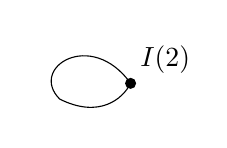
\begin{tikzpicture}[baseline=-2pt]\draw (0,0)..controls(-.5,.7)and(-1.3,.2)..(-.9,-.2)..controls(-.4,-.45)and(-.1,-.2)..(0,0);\fill(0,0) circle(2pt);\node[above right]at(0,0){$I(2)$};\end{tikzpicture}}}\arrow[r,"2"]\arrow[dr,"1"']\&
{\figure{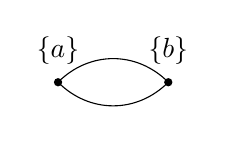
\begin{tikzpicture}[baseline=-2pt]\draw (0,0)..controls(.4,.4)and(1,.4)..(1.4,0);\draw (0,0)..controls(.4,-.4)and(1,-.4)..(1.4,0);\fill(0,0)circle(1.5pt);\fill(1.4,0)circle(1.5pt);\node[above]at(0,.1){$\{a\}$};\node[above]at(1.4,.1){$\{b\}$};\end{tikzpicture}}}=P_0\\
{\figure{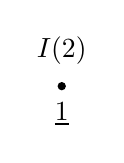
\begin{tikzpicture}[baseline=-2pt]\fill(0,0)circle(1.5pt);\node[above]at(0,.15){$I(2)$};\node[below]at(0,-.08){$\underline1$};\end{tikzpicture}}}\&
G_1={\figure{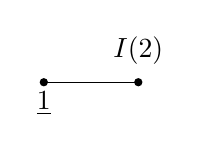
\begin{tikzpicture}[baseline=-2pt]\draw(0,0)--(1.2,0);\fill(0,0)circle(1.5pt);\fill(1.2,0)circle(1.5pt);\node[below]at(0,0){$\underline1$};\node[above]at(1.2,.1){$I(2)$};\end{tikzpicture}}}\arrow[r,"1"]\&
|[alias=scan070-p-one]|{\figure{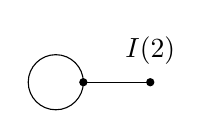
\begin{tikzpicture}[baseline=-2pt]\draw (0,0) circle(.35);\draw (.35,0)--(1.2,0);\fill(.35,0)circle(1.5pt);\fill(1.2,0)circle(1.5pt);\node[above]at(1.2,.1){$I(2)$};\end{tikzpicture}}}=P_1
\end{tikzcd}}\right.
\]
\margin{$D_\circ$ ``D boucle''\quad $D_{\bullet-\bullet}$ ``D segment''}
Il y a deux diviseurs à l'infini, \inserted{$D_\circ$ et $D_{\bullet-\bullet}$,} et deux points \inserted{critiques} à l'infini, \deleted{dont}\inserted{$P_0$ et $P_1$,} l'un \inserted{$P_0$} est contenu dans $D_\circ$ et dans $D_{\bullet-\bullet}$, et l'autre n'est contenu que dans $D_{\bullet-\bullet}$.

Essayons de \inserted{bien} saisir la structure de la multiplicité schématique à l'infini $\widehat M^\infty_{1,I}\simeq\widehat M^{!\,\infty}_{1,2}$, qui est la réunion amalgamée des deux multiplicités lisses \deleted{\unsure{$\widehat M$}} $D_\circ$ et $D_{\bullet-\bullet}$.
$D_\circ$ est isomorphe à $(\widehat M^{\unsure{!}}_{G_0},\Gamma^!_0)$, où $G_0$ est le \inserted{MD-}graphe
\figure{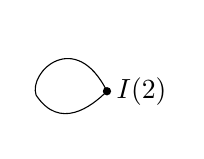
\begin{tikzpicture}[baseline=-2pt]\draw (0,0)..controls(-.4,.8)and(-1,.25)..(-.9,-.05)..controls(-.6,-.5)and(-.2,-.2)..(0,0);\fill(0,0)circle(1.5pt);\node[right]at(0,0){$I(2)$};\end{tikzpicture}},
$\Gamma_0$ son groupe d'automorphismes, et $\Gamma^!_0=\operatorname{Ker}(\Gamma_0\longrightarrow\mathfrak S_{I(G_0)})\simeq\mathbf Z/2$.
D'ailleurs $\widehat M_{G_0}\simeq\widehat M^!_{0,4}\simeq\mathbf P^1_{\mathbf Z}$, sur lequel $\Gamma^!_0\simeq\mathbf Z/2$ opère en fixant un des \inserted{trois} pts à l'infini de $U_{0,3\,\mathbf Z}$, \inserted{soit $1$,} et en transposant les deux autres, \inserted{soit $\{0,\infty\}$,} \deleted{De façon plus intrinsèque,} (ceci correspond au choix d'un élément de $I$ comme $1$, et les deux éléments de $\widetilde A(G_0)$ comme $0$ et $\infty$) donc on trouve le ``quotient'' par $z\longmapsto z^{-1}$. De façon
\margin{69}
\scanpage{71}
plus intrinsèque, le graphe $G_0$ \deleted{\unsure{se déploie}} \unsure{associe|associé} à l'ens $I\amalg\widetilde A'_0$ de card $4$, muni d'une partition de type $(2,2)$, (et \unsure{$=$} d'une partie \inserted{$I$} (de card $2$), l'ens \inserted{$J$} des \inserted{$3$} partitions de type $(2,2)$ a donc un pt marqué $\varepsilon_1$, les deux autres pts correspondent aux élts de l'ens $J':=I\wedge_{\mathbb Z/2}\widetilde A'_0$ :
\[
(84)\qquad J=\{\varepsilon_1\}\amalg J'\qquad J'=I\wedge_{\mathbb Z/2}\widetilde A'_0.
\]
Ceci posé, $\mathbb P^1_J=\mathbb P^1_{\{\varepsilon_1\}\amalg J'}\deleted{\unsure{\mathfrak S_{J'}}}$ peut être considéré comme le compactifié de $\mathbb G_m^{\unsure{1}}\wedge_{\pm1}J'$ et \deleted{$\unsure{\mathfrak S_2}$} $\mathfrak S_{J'}\simeq\mathbb Z/2$ y opère par transfert de structure. On a :
\margin{$\varepsilon_1$ correspond au point $1$}
\[
(85)\qquad
\left\{\begin{aligned}
\widehat M_{G_0}&\simeq(\mathbb P^1_{\{\varepsilon_1\}\amalg J'}\deleted{\unsure{\mathfrak S_{J'}}})\\
(\widehat M_{G_0},\unsure{\Gamma'_0})&\simeq(\mathbb P^1_{(\varepsilon_1\amalg J')},\mathfrak S_{J'})
\end{aligned}\right.
\]
\margin{$(\unsure{\widehat M_{D_0\bar\varepsilon}})$}
sur lesquels $\mathfrak S_I$ opère via $\mathfrak S_{J'}$, donc $\mathfrak S_I$ \uline{opère trivialt sur} $\widehat M_{D_0}$. Les deux pts à l'infini de $\widehat M_{D_0}$ correspondent : la trajectoire $J'$ d'une part \inserted{(pt. $P_0$)}, la trajectoire $\varepsilon_1$ d'autre part (point $P_1$). On a
\[
(86)\qquad M_{D_0}\simeq\unsure{\mathbb E^1_{\mathbb Z}|\mathbb A^1_{\mathbb Z}}\setminus\{\text{section }2\}=\operatorname{Spec}\mathbb Z[T]_{(T-2)}
\]
\[
\text{via}\quad\left\{\begin{aligned}M_{G_0}&\longrightarrow M_{D_0}\\ T&\longrightarrow T+\frac1T\end{aligned}\right.
\]
\[
(87)\qquad\widehat M_{D_0}\simeq\bigl(\mathbb P^1_{\mathbb Z},\text{ avec ``signature'' }2\text{ le long de la section }T=2\bigr)
\]
\margin{70}
\scanpage{72}
\mspage{35}
dans ce dernier iso, $P_0$ correspond à la section à l'infini, et $P_1$ à la section $2$ de $\mathbb P^1_{\mathbb Z}$.

D'autre part, on a
\[
(88)\qquad \widehat M_{D_1}=\widehat M_{G_1}\simeq\widehat M_{1,1}
\deleted{\simeq\bigl(\mathbb P^1_{\mathbb Z},\text{ avec signatures }4\text{ et }6\text{ le long des sections }0\text{ et }j_1=2^{\unsure{\alpha}}3^{\unsure{\beta}}\text{ (correspondant à la courbe elliptique d'autom }\unsure{\mathbb Z/6\mathbb Z|\mathbb Z/4\mathbb Z}\bigr)}
\]
\deleted{dans le dernier iso, \deleted{\unsure{lorsque}} la section à l'infini de $\widehat M_{D_1}$}

Je me rends compte qu'il me faudrait mieux comprendre la structure de $\widehat M_{1,1}$ (et \unsure{$=$} de $M_{1,1}$), à commencer dans le cadre transcendant (analytique complexe, avec \unsure{évt.} la structure réelle explicite -- i.e. considération de la conjugaison complexe\ldots). J'y reviendrai plus loin.

\uline{Notons déjà}

\uline{Proposition} Si $\dim M_G\geq2$, alors $M_G^\infty$ est \inserted{\unsure{géom.}} connexe \inserted{(fibre par fibre)}.

Dém. Écrivons
\[
(89)\qquad\left\{\begin{aligned}
\widehat M_G&\simeq\prod_{\alpha\in S}\widehat M^{\unsure{!|'}}_{g_\alpha,\widehat\nu_\alpha}\\
M_G&\simeq\prod_{\alpha\in S}M^{\unsure{!|'}}_{g_\alpha,\widehat\nu_\alpha}
\end{aligned}\right.
\]
\margin{71}
\scanpage{73}
et utilisant le fait que les $\widehat M^{!}_{g_\alpha,\widehat\nu_\alpha}$ sont connexes, on voit que $\widehat M_G^\infty=\widehat M_G\setminus M_G$ est connexe dès que \deleted{deux} parmi les facteurs $\widehat M^{!}_{g_\alpha,\widehat\nu_\alpha}$, il y en a au moins deux qui sont de dim $\geq1$ (en utilisant le fait que pour un tel $\alpha$, on a $M^\infty_{g_\alpha,\widehat\nu_\alpha}\ne\varnothing$). Donc il suffit de regarder le cas où $\widehat M_G\simeq\widehat M^{!}_{g,\nu}\inserted{\simeq\widehat M_{g,I}}$, avec \inserted{le cas où $3(g-1)+\nu=2$ est déjà vu, donc \unsure{DPS} $N\geq3$.} \inserted{$(\dim M_{g,\nu}=)$} $N=\unsure{2|3}(g-1)+\nu\geq2$. \deleted{Dans ce cas,} Il suffit de voir que deux diviseurs à l'infini peuvent être joints par une chaine de tels div. dont deux consécutifs ont une intersection non vide, compte tenu que ces diviseurs sont eux aussi connexes. Or les diviseurs à l'infini correspondent aux \deleted{types} \inserted{MD-}graphes suivants
\figure{\begin{tikzpicture}[x=1cm,y=1cm]
\node at (-1.5,-1.35) {$(90)$};
\draw (-.8,.8) .. controls (-1,.7) and (-.75,-.1) .. (-.95,-.4) .. controls (-1.05,-.55) and (-1.12,-.62) .. (-1.2,-.65) .. controls (-.83,-.7) and (-.8,-.95) .. (-.8,-1.2) -- (-.8,-2.5);
\node at (-.3,.25) {a)};
\fill (1,.25) circle (1.5pt);
\draw (1,.25) .. controls (1.75,.8) and (2.5,.75) .. (2.5,.25) .. controls (2.4,-.25) and (1.55,-.05) .. (1,.25);
\node[above] at (1,.4) {$I$}; \node[below] at (1,.15) {$g-1$};
\node at (4,.3) {$(\text{si }g\geq1)$};
\node at (-.3,-1.4) {b)};
\node at (1.6,-1.45) {\deleted{$\unsure{g'}$}};
\draw (1,-1.15)--(2.3,-1.8) (1,-1.8)--(2.1,-1.15) (1.15,-1.9)--(2.2,-1.25) (1.15,-1.25)--(2.45,-1.7);
\fill (2.8,-1.4) circle (1.5pt); \fill (4.1,-1.4) circle (1.5pt); \draw (2.8,-1.4)--(4.1,-1.4);
\node[above] at (2.8,-1.2) {$I'$}; \node[above] at (4.1,-1.2) {$I''$};
\node[below] at (2.8,-1.5) {$g'$}; \node[below] at (4.1,-1.5) {$g''$};
\node[anchor=north west,align=left] at (5,-1) {$\left\{\begin{aligned}
I&=I'\amalg I''\\
g'+g''&=\unsure{0|g}\\
&\deleted{2g'+\operatorname{card}I'\geq2}\\
&\deleted{2g''+\operatorname{card}I''\geq2}\\
&\inserted{\text{si }g'\text{ (resp }g'')=0,\text{ alors}}\\
&\inserted{\operatorname{card}I'\geq2\text{ (resp }\operatorname{card}I''\geq2\text{)}}
\end{aligned}\right.$};
\end{tikzpicture}}
\margin{72}
\scanpage{74}
\mspage{36}
On a comme spécialisation du cas a)
\figure{\begin{tikzpicture}[x=1cm,y=1cm]
\node at (-1,.1) {$(91)$}; \node at (0,.3) {$\unsure{a'}$)};
\fill (2,.2) circle (1.4pt); \fill (4,.2) circle (1.4pt);
\draw (2,.2)..controls (1.25,1.1) and (.25,.6)..(.6,-.1)..controls (.8,-.65) and (1.6,-.1)..(2,.2);
\draw (2,.2)--(4,.2); \draw (2.1,.35)..controls (2.8,.55) and (3.6,.55)..(3.9,.3);
\foreach \x in {2.2,2.35,...,3.8}{\draw (\x,.37)--(\x+.12,.5);}
\node[above] at (2,.65) {$I_1$};\node[below] at (2,.1) {$g_1$};
\node[above] at (4,.65) {$I_2$};\node[below] at (4,.1) {$g_2$};
\node[anchor=west,align=left] at (5.5,.15) {$\begin{gathered}I_1\amalg I_2=I\\g_1+g_2=g-1\\\text{si }g_2=0\quad\deleted{\unsure{quelconque}}\ \inserted{\text{on a }\operatorname{card}I_2\geq2}\\\deleted{\text{on a }I_1\ne\varnothing\text{ (et }I_2\ne\varnothing\text{)}}\end{gathered}$};
\end{tikzpicture}}
\margin{NB \unsure{OPS} $g_2=1$, $g_1=g-2$ pourvu que $g\geq2$; $(I_1,I_2)$ partition quelc. de $I$.}
On a comme spécialisation du cas b), \deleted{\unsure{si on suppose} $g'$}
\figure{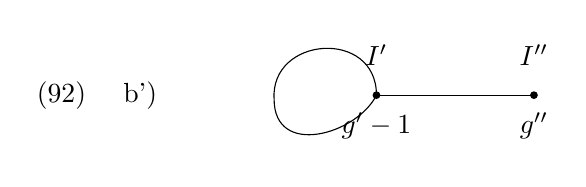
\begin{tikzpicture}[x=1cm,y=1cm]
\node at (-1,0) {$(92)$};\node at (0,0) {b')};
\fill (3,0) circle (1.4pt);\fill (5,0) circle (1.4pt);\draw (3,0)--(5,0);
\draw (3,0)..controls (3,.85) and (1.65,.75)..(1.7,-.05)..controls (1.7,-.8) and (2.75,-.5)..(3,0);
\node[above] at (3,.25) {$I'$};\node[below] at (3,-.1) {$g'-1$};
\node[above] at (5,.25) {$I''$};\node[below] at (5,-.1) {$g''$};
\end{tikzpicture}}
Donc si $g\geq1$ (de sorte que le cas a) existe) alors prenant dans b) \deleted{\unsure{avec} $g'\ne$} les notations $g',g''$ de sorte que $g'\ne0$ i.e. $g'\geq1$ (quitte à éch. $g',g''$), on voit que l'on a une spécialisation \inserted{b') $=$ a')} commune aux cas a) et b). Cela démontre notre assertion lorsque $g\ne0$. \deleted{Si $g$} Dans le cas $g=0$, \inserted{donc $\operatorname{card}I\geq6$}, il n'y a que les cas b), \deleted{et \unsure{OPS}} \deleted{\unsure{a il y a}} Or on a \deleted{\unsure{pour} $\operatorname{card}I'\geq\operatorname{card}I''$, donc $\operatorname{card}I'\geq3$; \unsure{qui a donc} la spécialisation} une spécialisation de la forme
\figure{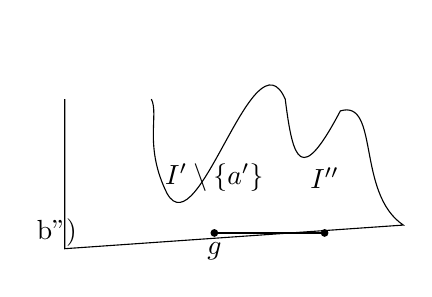
\begin{tikzpicture}[x=1cm,y=1cm]
\node at (0,0) {\deleted{b'')}};
\node at (2,.7) {\deleted{$I'\setminus\{a'\}$}};\node at (3.4,.7) {\deleted{$I''$}};
\fill (2,0) circle (1.4pt);\fill (3.4,0) circle (1.4pt);\draw (2,0)--(3.4,0);
\node[below] at (2,0) {\deleted{$\unsure{g}$}};
\draw (.1,1.7)--(.1,-.2)--(4.4,.1)..controls (3.8,.5) and (4.1,1.7)..(3.6,1.55)..controls (3.1,.6) and (3,0.9)..(2.9,1.7)..controls (2.5,2.6) and (1.8,-.2)..(1.4,.5)..controls (1.1,1.1) and (1.3,1.5)..(1.2,1.7);
\end{tikzpicture}}
\figure{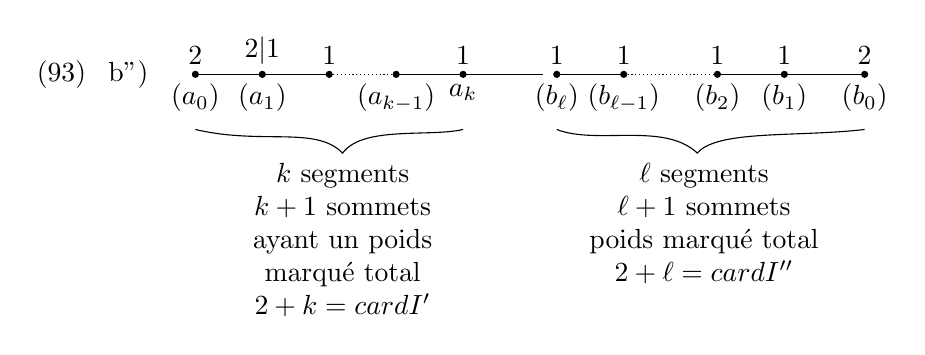
\begin{tikzpicture}[x=.85cm,y=1cm]
\node at (-2,0) {$(93)$}; \node at (-1,0) {b'')};
\draw (0,0)--(2,0) (3,0)--(5.2,0) (5.4,0)--(6.4,0) (7.8,0)--(10,0);
\draw[densely dotted] (2,0)--(3,0) (6.4,0)--(7.8,0);
\foreach \x in {0,1,2,3,4,5.4,6.4,7.8,8.8,10}{\fill (\x,0) circle (1.3pt);}
\node[above] at (0,0) {$2$};\node[below] at (0,0) {$(a_0)$};
\node[above] at (1,0) {$\unsure{2|1}$};\node[below] at (1,0) {$(a_1)$};\node[above] at (2,0) {$1$};
\node[below] at (3,0) {$(a_{k-1})$};\node[above] at (4,0) {$1$};\node[below] at (4,0) {$a_k$};
\node[above] at (5.4,0) {$1$};\node[below] at (5.4,0) {$(b_\ell)$};
\node[above] at (6.4,0) {$1$};\node[below] at (6.4,0) {$(b_{\ell-1})$};
\node[above] at (7.8,0) {$1$};\node[below] at (7.8,0) {$(b_2)$};
\node[above] at (8.8,0) {$1$};\node[below] at (8.8,0) {$(b_1)$};
\node[above] at (10,0) {$2$};\node[below] at (10,0) {$(b_0)$};
\draw (0,-.7)..controls (1,-.9) and (1.8,-.65)..(2.2,-1)..controls (2.5,-.65) and (3.5,-.8)..(4,-.7);
\draw (5.4,-.7)..controls (6,-.9) and (7,-.6)..(7.5,-1)..controls (7.8,-.7) and (9,-.8)..(10,-.7);
\node[anchor=north,align=center] at (2.2,-1) {$k$ segments\\$k+1$ sommets\\ayant un poids\\marqué total\\$2+k=\operatorname{card}I'$};
\node[anchor=north,align=center] at (7.6,-1) {$\ell$ segments\\$\ell+1$ sommets\\poids marqué total\\$2+\ell=\operatorname{card}I''$};
\end{tikzpicture}}
\margin{73}
\scanpage{75}
diagramme qui est déterminé, à isom. unique près, en se donnant un ordre total sur $I$, \inserted{(défini} mod \deleted{\unsure{interversion}} \inserted{transposition} des deux premiers él, et des deux derniers). Pour montrer que deux ordres totaux sur $I$ définissent \deleted{une} des pts de $M^\infty_{0,\nu}$ qui appartiennent à une $=$ composante connexe, il \inserted{suffit de} montrer que deux ordres totaux déduits l'un de l'autre par transposition des deux élts consécutifs \inserted{$c_i,c_{i+1}$} sont dans la $=$ composante connexe. Or on le voit en notant qu'on a deux morphismes de spécialisation \deleted{de} \inserted{dans}
\figure{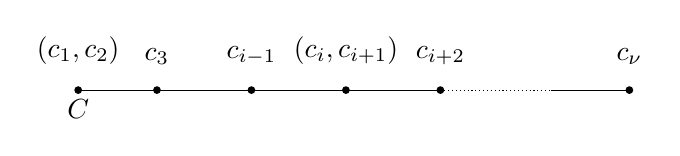
\begin{tikzpicture}[x=1cm,y=1cm]
\draw (0,0)--(1,0)--(2.2,0)--(3.4,0)--(4.6,0);
\draw[densely dotted] (4.6,0)--(6,0);\draw (6,0)--(7,0);
\foreach \x in {0,1,2.2,3.4,4.6,7}{\fill (\x,0) circle (1.4pt);}
\node[above] at (0,.2) {$(c_1,c_2)$};\node[below] at (0,0) {$C$};
\node[above] at (1,.2) {$c_3$};\node[above] at (2.2,.2) {$c_{i-1}$};
\node[above] at (3.4,.2) {$(c_i,c_{i+1})$};\node[above] at (4.6,.2) {$c_{i+2}$};
\node[above] at (7,.2) {$c_\nu$};
\end{tikzpicture}}
provient de
\figure{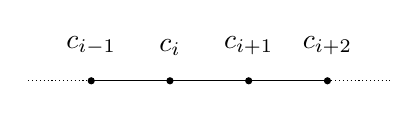
\begin{tikzpicture}[x=1cm,y=1cm]
\draw[densely dotted] (-.8,0)--(0,0) (3,0)--(3.8,0);\draw (0,0)--(1,0)--(2,0)--(3,0);
\foreach \x in {0,1,2,3}{\fill (\x,0) circle (1.3pt);}
\node[above] at (0,.2) {$c_{i-1}$};\node[above] at (1,.2) {$c_i$};
\node[above] at (2,.2) {$c_{i+1}$};\node[above] at (3,.2) {$c_{i+2}$};
\end{tikzpicture}}
et de
\figure{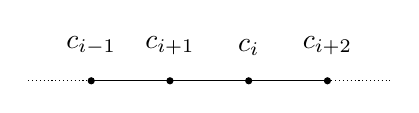
\begin{tikzpicture}[x=1cm,y=1cm]
\draw[densely dotted] (-.8,0)--(0,0) (3,0)--(3.8,0);\draw (0,0)--(1,0)--(2,0)--(3,0);
\foreach \x in {0,1,2,3}{\fill (\x,0) circle (1.3pt);}
\node[above] at (0,.2) {$c_{i-1}$};\node[above] at (1,.2) {$c_{i+1}$};
\node[above] at (2,.2) {$c_i$};\node[above] at (3,.2) {$c_{i+2}$};
\end{tikzpicture}}
en contractant la \deleted{\unsure{seg}} \inserted{arête} qui joint $c_i$ et $c_{i+1}$, OK.
\margin{74}
\scanpage{76}
\mspage{37}
9) \uline{La structure groupoïdale des \inserted{\uline{espaces modulaires de}} Teichmüller \unsure{modules|variétés}} (la \unsure{MDT|MDS}-structure) : cas transcendant, morphismes de générisation.

Nous travaillons maintenant avec les $M^{\mathrm{an}}_{g,\nu}$, $\widehat M^{\mathrm{an}}_{g,\nu}$ etc -- et pour ne pas traîner les exposants ``an'' (pour ``analytique''), nous les faisons tomber.

Considérons pour tout MD-graphe $\underline G$, la multiplicité modulaire (analytique) $M_{\underline G}$, et son groupoïde fondamental, que je note $\Pi M_{\underline G}$. C'est une \inserted{``grosse''} catégorie, par la suite nous allons voir comment la remplacer \inserted{\unsure{canoniqt}} par une \deleted{catégorie} \inserted{groupoïde} dont l'ens des objets soit fini. Dans nos constructions, il est en effet licite de remplacer un groupoïde tel que $\Pi M_{\underline G}$ par un groupoïde équivalent, pourvu que \deleted{l'équivalence} \inserted{dans celui-ci} \deleted{\unsure{un groupe}} \inserted{le groupe}
\[
(94)\qquad \Gamma_{\underline G}=\operatorname{Aut}\underline G
\]
opère, et que l'équivalence commute à l'action de ce groupe.

Notons déjà que $\Pi M_{\underline G}$ est un groupoïde
\margin{75}
\scanpage{77}
connexe, dont le $\pi_1$ est isomorphe (en tant que \uline{groupe extérieur}) :
\[
(95)\quad\pi_1(\Pi M_{\underline G})=\pi_1(M_{\underline G})\simeq\prod_{\alpha\in S(G)}\pi_1(M_{g_\alpha,\widehat I_\alpha})\simeq\prod_\alpha\mathcal T^+_{g_\alpha,I_\alpha}\simeq\prod_\alpha\mathcal T^{!+}_{g_\alpha,\nu_\alpha}.
\]
\margin{où les $\mathcal T^{!+}_{g,\nu}$ sont des groupes de Teichmüller}
Les opérations de $\unsure{\Gamma^{!}_{\underline G}|\Gamma_{\underline G}}$ sur $\Pi M_{\underline G}$ définissent un groupoïde mixte $(\Pi M_{\underline G},\Gamma_{\underline G})$, dont le groupe fondamental (extérieur) s'insère \deleted{de \unsure{par}} \inserted{dans} une structure d'extension
\[
(96)\quad1\longrightarrow\pi_1(\Pi M_{\underline G},\Gamma_{\underline G})\longrightarrow\pi_1(\Pi M_{\underline G},\Gamma_{\underline G})\unsure{-|\longrightarrow}\Gamma_G\longrightarrow1
\]
Nous allons définir une \inserted{sorte de} variance des $\Pi M_{\underline G}$ relativement à deux sortes de ``morphismes'' pour les MD-graphes $\underline G$. 

Tout d'abord une \uline{``variance de générisation''}, qui est composée de la \uline{variance pour isomorphismes} de MD-graphes (que j'admets comme ``triviale'', et qu'il est inutile de préciser) et une ``variance de passage au quotient de MD-graphes''.
\margin{76}
\scanpage{78}
\mspage{38}
Soit donc $\underline G'$ un MD-graphe quotient de $\underline G$ -- par un ens. \inserted{$C$} d'arêtes du graphe $G$ sous-jacent à $\underline G$,
\[
(96)\qquad\underline G'=\underline G/C.
\]
On a alors un \inserted{diagramme de} morphismes canoniques
\diagram{\begin{tikzcd}[ampersand replacement=\&, row sep=large,column sep=large]
\overset{\deleted{\unsure{\wedge}}}{M}_{\underline G}\arrow[d,hook]\arrow[r,phantom,"\deleted{\longrightarrow}"] \& \deleted{\unsure{\widehat M_{\underline G'}}}\arrow[d,phantom,"\deleted{\downarrow}"]\\
\widehat M_{\underline G}\arrow[r] \& \widehat M_{\underline G'}
\end{tikzcd}\quad(97)}
\margin{\unsure{développer|distinguer} la déf. de $\Gamma^!_{\underline G,\underline G'}$ !}
Si on désigne par $\Gamma^!_{\underline G,C}$ ou $\Gamma^!_{\underline G,\underline G'}$ le sous-groupe de $\Gamma_{\underline G}$ qui est formé des autom qui transforment $C$ en lui-$=$, et qui induisent l'identité sur $\underline G'$, la \unsure{flèche} \deleted{\unsure{verticale}} \inserted{horizontale} de (97) se factorise \deleted{donc} en une immersion de multiplicités
\diagram{\begin{tikzcd}[ampersand replacement=\&]
(\widehat M_{\underline G},\Gamma^!_{\underline G,\underline G'})\arrow[r,hook] \& \widehat M_{\underline G'}
\end{tikzcd}\quad(98)}
\margin{Ce ne sont peut-être que des immersions \uline{locales}, il me semble -- à vérifier\ldots}
Je désigne par $\widehat M_{\underline G,\underline G'}$ le \uline{germe de multiplicité} défini par l'inclusion (98), et par $M_{\underline G,\underline G'}$ le germe défini par l'inclusion induite
\diagram{\begin{tikzcd}[ampersand replacement=\&]
(M_{\underline G},\Gamma^!_{\underline G,\underline G'})\arrow[r,hook] \& \widehat M_{\underline G'}
\end{tikzcd}\quad(99)}
\margin{Il vaut mieux considérer le germe de multiplicité défini par l'\uline{immersion locale} $M_{\underline G}\longrightarrow\widehat M_{\underline G'}$, et faire opérer $\Gamma^!_{\underline G,\underline G'}$ dessus, \unsure{et ce sera} $M_{\underline G,\underline G'}$.}
\margin{77}
\scanpage{79}
Je désigne par $\widehat M^*_{\underline G,\underline G'}$, $\overset{\deleted{\unsure{\wedge}}}{M}{}^*_{\underline G,\underline G'}$ les germes de multiplicités obtenus en \deleted{enlevant (``l'infini'') $\widehat M_{\underline G}$ resp. $M_{\underline G}$, $\unsure{\Gamma^!_{\underline G,\underline G'}}$ (les traces de la \unsure{réunion} des diviseurs de $\widehat M_{\underline G'}$ \unsure{qui contiennent} $(\widehat M_{\underline G},\Gamma^!_{\underline G,\underline G'})$)}
\inserted{\deleted{prenant les traces de $M$} enlevant les traces des diviseurs à l'infini de $\widehat M_{\underline G'}$ \deleted{\unsure{non seuls}} qui contiennent $M_{\underline G}$ -- dans le cas de $M^*_{\underline G,\underline G'}$, on prend la \uline{trace} de $M_{\underline G'}$ sur $\widehat M_{\underline G,\underline G'}$.}
Ils sont donc des filtres d'ouverts de la multiplicité $M_{\underline G'}$, et les groupoïdes \unsure{fondamentals|fondamentaux} \deleted{$\unsure{\Pi}$}
\[
(100)\qquad\unsure{\Pi M^*_{\underline G,\underline G'}|\Pi\widehat M^*_{\underline G,\underline G'}},\qquad\Pi M^*_{\underline G,\underline G'}
\]
sont définis comme des Catégories $\underset{\longrightarrow}{\lim}$ des catégories de revêtements \unsure{universels}, ou comme des catégories des revêtts \unsure{du connexe} desdits germes de multiplicités (comparer [5], n°5, p. $768'$).

On a alors des diagrammes de germes de multiplicités analytiques
\diagram{\begin{tikzcd}[ampersand replacement=\&, column sep=large,row sep=large]
\& M^*_{\underline G,\underline G'}\arrow[r,dash]\arrow[d] \& M_{\underline G'}\deleted{\unsure{M}}\\
(M_{\underline G}\deleted{\unsure{,\Gamma^!}})\arrow[r,"{\text{(équiv. d'homotopie !)}}"'] \& M_{\underline G,\underline G'} \&
\end{tikzcd}\quad(101)}
donnant lieu à des morphismes de groupoïdes
\margin{78}
\scanpage{80}
\mspage{39}
\[
\tag{102}
\diagram{\begin{tikzcd}[ampersand replacement=\&, column sep=large,row sep=large]
\& \Pi M^*_{\underline G,\underline G'} \arrow[r] \arrow[d] \& \Pi M_{G'} \\
\Pi(M_G\deleted{,\unsure{\Gamma^!_{\underline G,\underline G'}}}) \arrow[r,"\simeq"] \& \Pi M_{G,G'}
\end{tikzcd}}
\]
\margin{ceci est une équivalence de groupoïdes}
qu'on va réécrire comme
\[
\tag{103}
\diagram{\begin{tikzcd}[ampersand replacement=\&, column sep=large,row sep=large]
\Pi M^*_{\underline G,\underline G'} \arrow[r,"\unsure{\psi_{\underline G,\underline G'}|\gamma_{\underline G,\underline G'}}"] \arrow[d,"\varphi_{G,G'}"] \& \Pi M_{G'} \\
\Pi(M_G\deleted{,\Gamma^!_{\underline G,\underline G'}})
\end{tikzcd}}
\]
\margin{« diagramme de générisation pour les groupoïdes fondamentaux, \unsure{pour} le quotient de $\underline G\to\underline G'$ »}
\deleted{pour la suite, il sera plus commode d'écrire $\Pi M_{G,G'}$ au lieu de $\Pi(M_G,\Gamma^!_{\underline G,\underline G'})$}

L'hom des groupoïdes $\varphi_{G,G'}$ a les propriétés de \deleted{\unsure{la}} l'hom sur les $\pi_1$ dans une fibration de base $(M_G\deleted{,\Gamma_{\underline G,\underline G'}\inserted{\text{op. de }\Gamma^!_{G,G'}}})$, \deleted{de} fibre un produit de disques épointés (ou de cercles, si on préfère) --- on peut considérer $\Pi M^*_{\underline G,\underline G'}$ comme une « \uline{extension} » canonique des groupoïdes $\Pi(M_G\deleted{,\Gamma^!_{\underline G,\underline G'}})$ par $\mathbf Z^C$, où $C$, on le rappelle, est l'ens. des \deleted{frontières}\inserted{arêtes} de $\underline G$

\margin{Attention, il faut regarder $\mathbf Z^C$ comme un syst. local sur $(M_G,\Gamma_{\underline G,\underline G'})$, via les op. de $\Gamma^!_{\underline G,\underline G'}$ sur $C$\ldots}
\margin{\uline{NB} $(M_G\deleted{,\Gamma_{\underline G,\underline G'}})$ est un $K(\pi,1)$, et par conséquent \unsure{dans|on a dans} la suite exacte des $\pi_1$ de la fibration \unsure{qui précède} \unsure{incluse, on a bien un $1$ à gauche|des inclusions et bien un $1$ à gauche}.}
\margin{79}
\scanpage{81}
qu'on a contracté pour former la générisation $\underline G'$. \deleted{\unsure{Plus}} (On reviendra sur la structure de cette extension, comme un produit fibré d'extensions, un peu plus bas\ldots) L'hom $\gamma_{\underline G\deleted{\unsure{'}},\underline G'}$ s'appelle \uline{l'hom de générisation sur les groupoïdes fondamentaux}, associé à l'hom de générisation $\underline G\to\underline G'$.

On va dégager une propriété de transitivité sur ces homs de générisation, pour un composé d'homs de générisation
\[
\tag{104}
\diagram{\begin{tikzcd}[ampersand replacement=\&]
\underline G \arrow[r] \& \underline G' \arrow[r] \& \underline G''
\end{tikzcd}}
\]
qui donne naissance à un diagramme de groupoïdes
\deleted{\[
\diagram{\begin{tikzcd}[ampersand replacement=\&, row sep=large,column sep=large]
\Pi M^*_{\underline G,\underline G'} \arrow[r] \arrow[d] \& {} \\
\Pi M_{\underline G}
\end{tikzcd}}
\]}
\margin{80}
\scanpage{82}
\mspage{(40)}
\[
\tag{105}
\diagram{\begin{tikzcd}[ampersand replacement=\&, column sep=small,row sep=large]
\Pi M^*_{G,\deleted{\unsure{G'}},G''}
 \arrow[rr,dashed] \arrow[d,dashed]
 \arrow[dd,bend right=35,"\varphi_{G,G''}"']
 \arrow[rrr,bend left=22,"\gamma_{G,G''}"]
\&\& \Pi M^*_{G',G''} \arrow[r,"\gamma_{G',G''}"] \arrow[d] \& \Pi M_{G''} \\
\Pi M^*_{\underline G,\underline G'} \arrow[r,"\gamma_{G,G'}"] \arrow[d]
\& \deleted{\unsure{\Pi M_{G'}}} \arrow[r,"\deleted{\mathrm{can}}"]
\& \begin{gathered}\Pi M_{G'\deleted{,G''}}\\(\simeq\Pi(M_{G'},\Gamma^!_{G',G''}))\end{gathered}
\& \text{(103) pour }(G',G'')\\
\Pi M_{G\deleted{,\unsure{G'}}} \& \text{(103)}
\end{tikzcd}}
\]
\margin{(2 cart)}
\deleted{$(\unsure{\simeq\Pi M})$}

Dans ce diagramme, on a \deleted{\unsure{enlevé|oublié}} laissé tomber les soulignés pour les MD-graphes, \deleted{et on a remplacé la notation $\Pi(M_{G,G'},\Gamma^!_{G,G'})$ par la notation plus légère $\Pi M_{G,G'}$, de $=$ pour $\Pi M_{G',G''}$.} On \deleted{\unsure{tire de (105)}}\deleted{a défini} \unsure{retrouve}
\[
\tag{106}
\Pi M^*_{G,G''\deleted{,\unsure{G'}}}
\]
dans (105) comme un produit 2-cartésien --- c'est donc un groupoïde connexe, ext. de $\Pi M^*_{G,G'}$ par un $\mathbf Z^{C'}$ (tordu), et il se trouve que c'est aussi, \unsure{en tant qu'ext.} de $\Pi M_{G\deleted{,\unsure{G'}}}$ (de noyau une ext. de $\mathbf Z^C$ tordu par $\mathbf Z^{C'}$ tordu) une extension de $\Pi M_{G\deleted{,\unsure{G'}}}$ par un $\mathbf Z^{C\amalg C'}$ tordu.

De façon plus précise, on tire de (105) le diagramme
\[
\tag{107}
\diagram{\begin{tikzcd}[ampersand replacement=\&, column sep=large,row sep=large]
\Pi M^*_{G,\deleted{\unsure{G'}},G''} \arrow[r,dash,"\gamma_{G,\deleted{\unsure{G'}},G''}"] \arrow[d,dash,"\varphi_{G,G''\deleted{,\unsure{G'}}}"] \& \Pi M_{G''} \\
\Pi M_{G\deleted{,\unsure{G'}}}
\end{tikzcd}}
\]
\margin{81}
\scanpage{83}
\deleted{que je voudrais comparer au diagramme de \deleted{spécialisation}\inserted{générisation} pour $G'\unsure{-|\to}G''$ :
\[
\tag{108}
\diagram{\begin{tikzcd}[ampersand replacement=\&, column sep=large,row sep=large]
\Pi M^*_{G,G''} \arrow[r,"\gamma_{G'',G}"] \arrow[d,"\varphi_{G,G''}"] \& \Pi M_{G''} \\
\Pi M_{G\deleted{,\unsure{G''}}}
\end{tikzcd}}
\]}

\deleted{Pour ceci, notons qu'on a un morphisme canonique
\[
\tag{109}
\diagram{\begin{tikzcd}[ampersand replacement=\&]
\Pi M_{G,G'} \arrow[r] \& \Pi M_{G,G''}
\end{tikzcd}}
\]
qu'on peut décrire, soit via \deleted{\unsure{l'inclusion}}\inserted{le morphisme} canonique de germes de multiplicités
\[
\diagram{\begin{tikzcd}[ampersand replacement=\&]
M_{G,G'} \arrow[r,hook] \& M_{G,G''},
\end{tikzcd}}
\]
soit, mieux, en \unsure{notant} qu'on a
\[
\tag{110}
\Gamma^!_{G,G'}\subset\Gamma^!_{G,G''}
\]
d'où
\[
\tag{111}
\diagram{\begin{tikzcd}[ampersand replacement=\&, column sep=large,row sep=large]
\Pi(M_G,\Gamma^!_{G,G'}) \arrow[r,"\mathrm{can}"] \arrow[d,"\sim"'] \& \Pi(M_G,\Gamma^!_{G,G''}) \arrow[d,"\sim"] \\
M_{G,G'} \& M_{G,G''}
\end{tikzcd}}
\]}

Ceci posé, \deleted{je dis} on aura un diagramme, \deleted{que je} est commutatif
\margin{82}
\scanpage{84}
\mspage{(41)}
\deleted{\[
\tag{112}
\diagram{\begin{tikzcd}[ampersand replacement=\&, column sep=large,row sep=large]
\Pi M^*_{G,G',G''} \arrow[rr,"\gamma_{G,G',G''}"] \arrow[dr] \arrow[dd] \&\& \Pi M_{G''} \arrow[dr,Rightarrow] \\
\& \Pi M^*_{G,G''} \arrow[rr,"\gamma_{G,G''}"] \arrow[dd] \&\& \Pi M_{G''}\\
\Pi M_{G\deleted{,\unsure{G'}}} \arrow[dr,Rightarrow,"\mathrm{can}"'] \\
\& \Pi M_{G,G''}
\end{tikzcd}}
\]
où le carré vertical est 2-cartésien. En d'autres termes, le produit 2-cartésien $\Pi M^*_{G,G',G''}$ défini formellement via (105) comme composé de deux extensions successives de $\Pi M_{G,G'}$, s'interprète canoniquement comme l'extension image inverse de $\Pi M^*_{G,G''}$ sur $\Pi M_{G,G''}$ par
\[
\diagram{\begin{tikzcd}[ampersand replacement=\&]
\Pi M_{G,G'} \arrow[r] \& \Pi M_{G,G''}.
\end{tikzcd}}
\]}

Considérons maintenant le cas d'un morphisme de générisation $G\to G'$, où $G'$ est le graphe de MD \uline{discret} défini par $G$ --- c'est donc la \deleted{\unsure{spécial}}\inserted{générisation} « la plus grossière » de toutes. On \deleted{désignera}\inserted{posera} \deleted{par $S\Pi\unsure{\mathfrak G|\Gamma}M_G$}
\margin{83}
\scanpage{85}
\[
\tag{113}
S_A\Pi M_G\overset{\mathrm{def}}=\Pi M^*_{G,G'},
\]
\margin{ici $A$ désigne l'ens. de toutes les arêtes de $G$.}
\unsure{$\ast$} c'est donc une extension de $\Pi M_{G,G'}$ \margin{$=$\deleted{$(\Pi(M_G,\unsure{\Gamma_G}))$}} par $\mathbf Z^{A(G)}$ \deleted{de}, où $A(G)$ est l'ens. des arêtes de $G$.

Bien entendu, le groupe $\Gamma=\operatorname{Aut}G$ opère non seulement sur $M_G$ et sur $\Pi M_G$, mais aussi sur $S_A\Pi M_G$ \deleted{$=\Gamma$} (via son action sur $M^*_{G,G'}$), de façon à commuter au morphisme canonique
\[
\tag{114}
\diagram{\begin{tikzcd}[ampersand replacement=\&]
S_A\Pi M_G \arrow[r] \& (\Pi M_G\deleted{,\Gamma_G})
\end{tikzcd}}
\]
ce qui permet, pour $\forall$ sous-groupe \deleted{$\Gamma'$}
\[
\Gamma'\subset\Gamma_G
\]
de définir une extension
\margin{expliciter un peu\ldots}
\[
\tag{115}
\diagram{\begin{tikzcd}[ampersand replacement=\&, column sep=large,row sep=small]
(S_A\Pi M_G,\Gamma') \arrow[r] \& (\Pi M_G,\deleted{\unsure{\Gamma_G}}\inserted{\Gamma'})\\
\text{ou } S_A\Pi(M_G,\Gamma') \arrow[r,dash] \& \Pi(M_G,\Gamma')
\end{tikzcd}}
\]
\deleted{Soit $C$ un ensemble d}
dont le « noyau » est le système local $\mathbf Z^{A(G)}$ sur $(\Pi M_G,\Gamma')$, tordu grâce à l'action de $\Gamma'$ sur $A(G)$. Si $C\subset A(G)$ est stable par l'action de $\Gamma'$, alors on a un hom
\[
\tag{116}
\diagram{\begin{tikzcd}[ampersand replacement=\&]
\mathbf Z^{A(G)} \arrow[r] \& \mathbf Z^C
\end{tikzcd}}
\]
\margin{84}
\scanpage{86}
\mspage{42}
de systèmes locaux, qui permet de construire une extension quotient de $(S\Pi M_G,\Gamma')$, extension du groupoïde $(\Pi M_G,\Gamma')$ par $\mathbf Z^C$, qu'on va noter
\[
\tag{117}
(S_C\Pi M_G,\Gamma').
\]
\deleted{Dans le cas où $\Gamma'=\Gamma^!_{G,G'}$, avec $G'=G/C$, on retrouve l'extension $\Pi M^*_{G,G'}$ de $\Pi M_{G,G'}$ par $\mathbf Z^C$ (tordu).
\[
\tag{118}
(S_C M_G,\Gamma_{G,G/C})\simeq\Pi M^*_{G,G/C}.
\]}

On va plutôt expliciter les données en termes de
\[
\diagram{\begin{tikzcd}[ampersand replacement=\&]
S_A\Pi M_G \arrow[r] \& (\Pi M_G,\unsure{\Gamma_G^!|\Gamma_G})
\end{tikzcd}}
\]
Si $G'\inserted{\simeq G/C}$ est une \deleted{spécialisation}\inserted{générisation} de $G$, alors on a
\[
\tag{11\unsure{9|8}}
\diagram{\begin{tikzcd}[ampersand replacement=\&]
S_A\unsure{\Pi}M_G \arrow[r] \& S_{A'}\Pi M_{G'},
\end{tikzcd}}
\]
qui passe aux quotients en
\[
\tag{120}
\diagram{\begin{tikzcd}[ampersand replacement=\&, column sep=large,row sep=large]
S_{\inserted{A}}\deleted{A}\Pi M_G \arrow[r,dash,"\gamma_{G,G'}"] \arrow[d] \& S_{A'}\Pi M_{G'} \arrow[d] \\
S_C\Pi M_G\deleted{\Gamma'} \arrow[r] \& \Pi M_{G'}
\end{tikzcd}}
\]
compatible avec l'action de $\Gamma_{G,G'}$, \unsure{donc|dont} \deleted{\unsure{que}} la deuxième flèche horizontale à son tour
\margin{85}
\scanpage{87}
se factorise en
\[
\tag{121}
\diagram{\begin{tikzcd}[ampersand replacement=\&, column sep=large]
\underbrace{(S_C\Pi M_G,\Gamma^!_{G,G'}\deleted{\unsure{\prime}})}_{\deleted{\Pi M^*_{G,G'}}} \arrow[r] \& \Pi M_{G'},
\end{tikzcd}}
\]
\deleted{que}\inserted{et} plus généralement, si $\Gamma^!_{G,G'}\subset\Gamma'\subset\Gamma_{G,G'}$ est un sous-groupe de $\Gamma=\operatorname{Aut}G$ qui stabilise $C$ et contient $\Gamma^!_{G,G'}$, on trouve
\[
\tag{122}
\diagram{\begin{tikzcd}[ampersand replacement=\&, column sep=large,row sep=large]
(S_{\unsure{S|C}}\Pi M_G,\Gamma') \arrow[r] \arrow[d,equal] \& (\Pi M_{G'},\Gamma'/\Gamma^!_{G,G'})\\
(\Pi M_{G,G'},\Gamma'/\Gamma^!_{G,G'})
\end{tikzcd}}
\]

Ici la relation de transitivité un peu compliquée \inserted{(105)} s'exprime, plus simplement, par le fait que les \inserted{groupoïdes} $S_A\Pi M_G$ dépendent fonctoriellement des \inserted{MD-}graphes $G$, pour les morphismes de générisation.

On va axiomatiser un peu. \deleted{plus.} Les MD-graphes \inserted{et morphismes de générisation} forment une \uline{catégorie}, $(\deleted{\unsure{\mathcal G}}\mathfrak g)$, où tous les morphismes sont des épimorphismes. Cette catégorie satisfait
\margin{La catégorie $\mathcal G$ joue le rôle d'un ens. de \unsure{complexités|« types »} géométriques \unsure{ou des cas}\ldots}
\margin{86}
\scanpage{88}
\mspage{43}
à la condition suivante

(123) (Simp) Pour $\forall\ G\in\unsure{\mathcal M|\mathfrak g}$, l'ens. ordonné des quotients \inserted{$G'$} de $G$ est \deleted{isomorphe à un \unsure{simplexe}}\inserted{un « simplexe », i.e. isomorphe} \unsure{à} un ens. des parties d'un ens. fini.

Si $A_G$ désigne l'ens. des quotients de $G$ qui sont $\ne G$ et qui sont \deleted{minimaux}\inserted{maximaux} parmi ceux-ci, alors l'ens. \inserted{ordonné} des quotients de $G$ est donc isomorphe à l'ens. des parties de $A_G$. \deleted{Si} On désigne par $G/C$ le quotient de $G$ associé à $A_G\setminus C$ (d'autant plus petit que $C$ est plus grand).

\margin{\uline{NB} Il faudrait montrer comment cette axiomatisation s'applique à \unsure{$\forall$|la} situation de multiplicités, \deleted{topologiques ou \unsure{étales}}\inserted{\unsure{analytiques relatives|algébriques relatives}} avec un diviseur à croisements normaux\ldots (à cela près que $S\Pi M_G$ est une extension de $\Pi M_G$ non pas par un $\mathbf Z^C$ tordu, mais par un quotient d'un tel\ldots}

On suppose donné pour $\forall\ G\in\operatorname{Ob}\mathcal G$ deux groupoïdes $S\Pi M_G$ et $\Pi M_G$, et un morphisme
\[
\tag{124}
\diagram{\begin{tikzcd}[ampersand replacement=\&]
S\Pi M_G \arrow[r,dash,"\varphi_G"] \& \Pi M_G.
\end{tikzcd}}
\]
On suppose que $\varphi_G$ fait de $S\Pi M_G$ une extension de $\Pi M_G$ par $\mathbf Z^{A(G)}$ (en fait, c'est une structure supplémentaire sur $S\Pi M_G$). On suppose que $G\mapsto\Pi M_G$ est un foncteur en $G$ \uuline{pour les iso} (pas pour les morphismes quelc.).
\margin{87}
\scanpage{89}
et que $\inserted{G\mapsto}S\Pi M_G$ est un foncteur en \deleted{$M_G$} $G$ pour les morphismes quelconques, et que (124) est fonctoriel pour les iso. Pour un morphisme quelconque $G\xrightarrow{f}G'$, correspondant à une partie $C\subset A_G$ (telle que $G\unsure{-|\to}G'$ soit isom., en tant que quotient de $G$, à $G\unsure{-|\to}G/C$), on suppose que l'on a un diagramme commutatif
\[
\tag{125}
\diagram{\begin{tikzcd}[ampersand replacement=\&, column sep=large,row sep=large]
S\Pi M_G \arrow[r,"S\Pi(f)"] \arrow[d,"\varphi_G"] \& S\Pi M_{G'} \arrow[d,"\varphi_{G'}"] \\
S_{\unsure{C|A}}M_G \arrow[r,"\gamma_f"] \& \Pi M_{G'}
\end{tikzcd}}
\]
i.e. que le composé
\[
\diagram{\begin{tikzcd}[ampersand replacement=\&, column sep=large]
S\Pi M_G \arrow[r,"S\Pi(f)"] \& S\Pi M_{G'} \arrow[r,dash,"\varphi_{G'}"] \& \Pi M_{G'}
\end{tikzcd}}
\]
se factorise par l'extension $S_{\unsure{C|A}}M_G$ de $\Pi M_G$ par $\mathbf Z^C$, déduite de l'extension $S\Pi M_G$ de $\Pi M_G$ par $\mathbf Z^{A(G)}$ grâce à l'hom canonique
\[
\diagram{\begin{tikzcd}[ampersand replacement=\&]
\mathbf Z^{A(G)} \arrow[r] \& \mathbf Z^C.
\end{tikzcd}}
\]
On a \unsure{automatiquement|automatique} alors la relation de transitivité pour un composé.
\margin{88}
\scanpage{90}
\mspage{44}
10) \uline{Structure} MDT \uline{discrète} : \uline{action} des \uline{morphismes de normalisation entre \inserted{MD-}graphes}.

Nous voulons exprimer, en plus des morphismes \deleted{$\varphi_G$ et} $S\Pi f$ ($f$ morphisme de générisation) et $\Pi f$ ($f$ iso de MD-graphes) entre autres \unsure{des|ces} morphismes du type
\[
\diagram{\begin{tikzcd}[ampersand replacement=\&]
M_G \arrow[r] \& M_{g_\alpha,\widehat I_\alpha}
\end{tikzcd}}
\]
et
\[
\diagram{\begin{tikzcd}[ampersand replacement=\&]
M^{\unsure{?|!}}_{g,\unsure{I|\overline I}} \arrow[r] \& M_{g,I'}
\end{tikzcd}}
\qquad\text{pour }I'\subset I.
\]
On va introduire pour ceci une autre notion de morphismes de MD-graphes, qu'on appellera morphismes de normalisation (l'intersection des deux notions de morphisme est celle d'iso de MD-graphes).

Géométriquement, cela correspondra à la situation d'une courbe stable \deleted{$(\widehat X,I)$}\inserted{$X=\widehat X\setminus I$} sur un corps alg. clos $\unsure{k|h}$, en distinguant une partie $I'\subset I$ de l'ens. des pts à l'infini, et une partie $A'\subset A$ de l'ens. des pts doubles de $X$,
\margin{89}
\scanpage{91}
et en considérant la courbe $X'$, ayant $I'$ comme ensemble de pts à l'infini, et $A'$ comme ens. des pts doubles, obtenue en « bouchant les trous » relatifs aux $i\in I\setminus I'$, \deleted{\unsure{et|en}} et en normalisant $X$ en les pts de $A\setminus A'$. On trouve donc $X'=\widehat X'\setminus I'$, $\widehat X'$ étant la normalisée de $\widehat X$ relatif aux pts de $A\setminus A'$. On fera attention que $\overset{\deleted{\wedge}}{X}'$ \uline{ne s'envoie pas} dans $\overset{\deleted{\wedge}}{X}$ (sauf si $I'=I$), mais seulement dans $\widehat X$.

\deleted{On peut aussi aller plus loin, et} La construction de $X'$ en termes de $X$ est donc explicite, dès qu'on a donné des parties $I'\subset I$ et $A'\subset A$ --- cela revient, en termes du \deleted{\unsure{le graphe}} graphe associé à $X$, à se donner

\noindent a) un sous-graphe \inserted{$G'$} de $G$ ayant $=$ ensemble des sommets

\noindent b) un sous-ens. $I'$ de $I$.

\deleted{Mais \unsure{on}} Le graphe de $X'$ est donc le sous-graphe en question. Le \deleted{MD}-\unsure{marquage|marqué}
\margin{90}
\scanpage{92}
\mspage{45}
complet de $X'$ se déduit de celui de $X$, en prenant la $=$ application genre, et $I'\longrightarrow S$ induit par $I\longrightarrow S$.

En fait, quand on a normalisé $\widehat X$ en les pts de $\unsure{A|A^{a}}\setminus A'$ pour obtenir $\widehat X'$, on a sur $\widehat X'$, en plus des pts marqués indexés par $I$ et des pts \deleted{quadratiques}\inserted{doubles} indexés par $A'$, un troisième ens. remarquable de « pts marqués », savoir l'image inverse \inserted{$\unsure{\widetilde J|\widehat J}$} de $J=A\setminus A'$, \deleted{E} de cardinal égal à $2\operatorname{Card}(A\setminus A')$. En termes de la courbe normale propre $Y$ \deleted{qui} contenant $\widetilde A\amalg I$, qui définit $\widehat X$ comme $Y/\sigma_{\widetilde A}$ et $X$ comme $(Y\setminus I)/\sigma_{\widetilde A}$, $\unsure{\widehat X'|X'}$ est défini comme $Y/\sigma_{\widetilde A'}$, ce qui nous donne un ens. de pts marqués lisses \deleted{$\unsure{A}$} $\widetilde J\amalg I$ sur $\widehat X'$. Ceci étant, on peut « oublier » $\widetilde J$ et $I\setminus I'$ pour ne retenir que l'ens. de pts marqués
\margin{91}
\scanpage{93}
$I'$ sur $\widehat X'$, on peut aussi, plus généralement, se donner une partie $I'$ (non pas de $I$, mais de) $\widetilde J\amalg I$, qu'on \unsure{retiendra} comme ``pts marqués''.

Quand on s'est ainsi donné (pour un \deleted{\unsure{MD}}m.graphe $\underline G$ donné) une partie $A'$ de $A(G)$, et une partie $I'$ de $I\amalg\widetilde J$ (où $\widetilde J=\widetilde A(G)-\widetilde A'\deleted{\unsure{)}}$), alors pour la courbe spéciale $G$-épinglée, on déduit une courbe spéciale, qui sera épinglée par le m.graphe $\underline G'$ déduit de $\underline G,A',I'$ en prenant le sous-graphe \inserted{$G'$ de $G$} ayant \unsure{$=$|les} $S$ sommets et ayant $A'$ comme ens. d'arêtes, avec comme ``ens de pts marqués'' $I'\subset I\amalg\widetilde J$, qui s'envoie dans $S$ \deleted{\unsure{si}} par
\[
(120)\qquad I'\longrightarrow S\quad\text{induit par }I\longrightarrow S\text{ et }\widetilde A(G)\xrightarrow{\text{origine}}S,
\]
l'application genre pour $\underline G'$ est celle pour $\underline G$.
\margin{92}
\scanpage{94}
\mspage{46}
On peut généraliser encore un peu ces constructions, en \deleted{choisissant une \unsure{partie}} \inserted{remplaçant $\unsure{X'|\widehat X}$ par} \inserted{une réunion de composantes connexes} \deleted{de composantes irréductibles}, contenant $A'$ et $I'$. Cela revient à prendre un sous-graphe \uline{quelconque} $G'$ de $G$ (n'ayant pas $\text{néc}^{\text{t}}$ \deleted{\unsure{les}} $=$ ens. de sommets, mais un ens. de sommets $S'\subset S$), [défini donc par la donnée d'une partie $S'$ de $S$, d'une partie $\widetilde A'$ de $\widetilde A(G)$ \unsure{st.ble} par $\sigma_{\widetilde A}$ et telle que $o_G:\widetilde A\longrightarrow S$ applique $\widetilde A'$ dans $S'$], plus une partie $I'$ de $I\amalg\deleted{\widetilde A}\widetilde J$ (où $\widetilde J=\widetilde A\setminus\widetilde A'$), appliquée dans $S'$ par l'\deleted{application origine}\inserted{application}
\[
I\amalg\widetilde J\longrightarrow S\quad\text{induite par }I\longrightarrow S\text{ et par }\widetilde A\xrightarrow{o_G}S.
\]

Un cas particulièrement important est celui où $G'$ est un sous-graphe ponctuel, défini par un $\alpha\in S$, \inserted{donc $\widetilde J=\widetilde A$,} et où on prend
\[
I'=I_\alpha\amalg\widetilde A_\alpha=\text{image inverse de }\{\alpha\}\text{ par }I\amalg\widetilde A\longrightarrow S.
\]

Si on veut exprimer ces constructions en termes d'une notion ad-hoc de
\margin{93}
\scanpage{95}
``morphisme'' (de normalisation) de m.graphes, on aboutit à la

\uline{Définition} Soient $\underline G=(\underbrace{S,\widetilde A,\sigma_{\widetilde A},o_G}_{G},I\longrightarrow S\overset{g}{\unsure{-|\longrightarrow}}\mathbb N)$ et $\underline G'=(\underbrace{S',\ldots}_{G'})$ deux m.graphes. On appelle \uline{morphisme de \deleted{\unsure{pré}}normalisation} de $\underline G'$ dans $\underline G$ la donnée d'un couple \deleted{\unsure{f_G}} $(f_G,f_I)$, où

a) $f_G:G'\longrightarrow G$ est un hom. de graphes, qui est injectif sur les sommets et injectif sur l'ens des arêtes (donc identifie $G'$ à un sous-graphe de $G$)

\margin{On suppose de plus c) $\forall s'\in S',\quad g'(s')=g(f_G(s'))$}

b) $f_I:I'\longrightarrow I\amalg\widetilde A\deleted{(G)}$ est une application injective, dont l'image est contenue \unsure{dans} $I\amalg\widetilde J$, avec $\widetilde J=\widetilde A(G)\setminus f_G(\widetilde A'\deleted{\unsure{(G')}})$ et rendant commutatif le diagramme
\[
(129)\qquad
\diagram{\begin{tikzcd}[ampersand replacement=\&, row sep=small,column sep=large]
I' \arrow[r,hook] \arrow[d] \& I\amalg\unsure{A|\widetilde A} \arrow[d] \\
S' \arrow[r,hook,"\unsure{\forall}" description] \& S
\end{tikzcd}}
\]
\margin{On dit que $f$ est un \uline{morphisme de normalisation strict} si $S'\xrightarrow{\sim}S$, et si $I'\xrightarrow{\sim}I\amalg\widetilde J$.}

Par exple, \unsure{iso.} de m.graphes est un morphisme de normalisation. \deleted{\unsure{On}}

Voici une façon de raccorder cette notion à une notion ``orthodoxe'' de morphisme de graphes, en mettant ``dans un même sac'', pour un m.graphe
\margin{94}
\scanpage{96}
\mspage{47}
donné $G$, l'ens $\widetilde A(G)$ et $I(G)$ (munis l'un et autre d'une application \inserted{``origine''} à valeurs dans $S(G)$).

Pour ceci, on a à utiliser la notion de ``graphes avec branches \unsure{orphelines|aplaties}'', qui généralise celle de graphe, et topologiquement correspond à la classification des \deleted{\unsure{4}} couples $(X,S)$ d'un espace topologique compact $X$, et d'une partie finie $S$, tels que a) $X$ soit une étoile au voisinage de tt pt de $S$, \deleted{et} b) \deleted{\unsure{S}} tt composante connexe de $X\setminus S$ est une $1$-variété à bord non compacte (car on veut que \unsure{toute|tout} \deleted{adhérence} d'arête ait un sommet). Il revient au $=$ de dire que $X$ est un $1$-complexe top, et $S$ une partie finie qui contient les sommets d'ordre $\geq3$, et telle qu'aucune composante connexe de $X\setminus S$ ne soit compacte (i.e. que tt composante connexe de $X$ contienne un sommet, i.e. $S\longrightarrow\pi_0(X)$ est surjectif).

Ceci se classifie combinatoirement par des systèmes $(S,\unsure{\widehat A|\widehat I},\sigma_{\unsure{\widehat A|\widehat I}},o_{\unsure{\widetilde A|\widehat A}})$, où \deleted{$\unsure{\widetilde A=\sigma_{\widetilde A}}$} $S,\unsure{\widehat A|\widehat I}$ sont des ens finis, $\sigma_{\widehat A}$ est une involution de $\widehat A$, et $o_{\unsure{\widetilde A|\widehat A}}:\widehat A\unsure{-|\longrightarrow}S$ une
\margin{95}
\scanpage{97}
application. On n'exige plus que $\sigma_{\unsure{\widehat I|\widehat A}}$ soit sans pts fixes — l'ens des pts fixes, $I$, \deleted{se} correspond aux ``branches orphelines'' du $1$-complexe i.e. aux \deleted{``\unsure{bouts}''} ``pts-bord'' de $X$ qui ne sont pas dans $S$. La donnée d'un graphe à branches orphelines revient donc (en décomposant $\widehat I$ en $I\amalg\widetilde A$, où $I=\widehat I^\sigma$ et $\widetilde A=\widehat I\setminus\unsure{\widehat I^\sigma|I}$) à la donnée d'un \deleted{couple} graphe ordinaire \inserted{$(S,\widetilde A,\sigma_{\widetilde A},o_{\widetilde A})$}, plus un ensemble $I$ et une application $I\longrightarrow S$.

On décrit un tel graphe à branches orphelines par un graphisme tel que
\figure{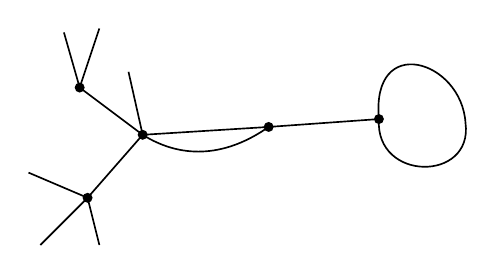
\begin{tikzpicture}[x=1cm,y=1cm,line width=.6pt]
\coordinate (a) at (0,0); \coordinate (b) at (-.8,.6); \coordinate (c) at (-.7,-.8); \coordinate (d) at (1.6,.1); \coordinate (e) at (3,.2);
\draw (a)--(b) (a)--(c) (a)--(d)--(e);
\draw (a) to[out=-32,in=-145] (d);
\draw (e) .. controls (2.9,1.3) and (4.05,.95) .. (4.1,.15) .. controls (4.2,-.6) and (2.95,-.6) .. (e);
\draw (b)--(-1,1.3) (b)--(-.55,1.35) (c)--(-1.45,-.48) (c)--(-1.3,-1.4) (c)--(-.55,-1.4) (a)--(-.18,.8);
\foreach \p in {a,b,c,d,e} {\fill (\p) circle (1.8pt);}
\end{tikzpicture}}
où les sommets sont figurés par des points gros $\bullet$, et les branches orphelines \deleted{sont} se distinguent par le fait justement qu'elles ne sont pas marquées \inserted{en} gros. Le graphe \inserted{à \unsure{b.o.|b.a.}} ci-dessus correspond donc, avec la notion des ``pieds marqués'', à
\figure{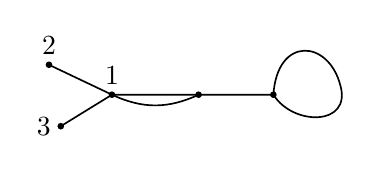
\begin{tikzpicture}[x=1cm,y=1cm,line width=.6pt]
\coordinate (a) at (0,0); \coordinate (b) at (-.8,.38); \coordinate (c) at (-.65,-.4); \coordinate (d) at (1.1,0); \coordinate (e) at (2.05,0);
\draw (b)--(a)--(c) (a)--(d)--(e);
\draw (a) to[out=-25,in=-155] (d);
\draw (e) .. controls (2.1,.75) and (2.75,.7) .. (2.9,.12) .. controls (3.05,-.4) and (2.3,-.4) .. (e);
\foreach \p in {a,b,c,d,e} {\fill (\p) circle (1.2pt);}
\node[above] at (a) {$1$}; \node[above] at (b) {$2$}; \node[left] at (c) {$3$};
\end{tikzpicture}}
\margin{96}
\scanpage{98}
\mspage{48}
Dans cette optique, on voit que dans le cas où \inserted{$S'\simeq S$,} $I'\xrightarrow{\sim}I\amalg\widetilde J$, on obtient $G'$ à partir de $G\deleted{\unsure{'}}$ en se donnant l'ens. $C$ de \deleted{\unsure{pieds}}\inserted{arêtes (ordinaires)}, de $G\deleted{\unsure{'}}$ qu'on veut ``enlever'' (\inserted{$\widetilde C$ est le} complémentaire de $\unsure{I'|\widetilde A'}$ \unsure{ds|et} $(\widehat I'\longrightarrow\widehat I)$) en prenant un pt sur chaque arête $\in C$, et en ``coupant'' l'arête en ce point avec un coup de ciseaux (i.e. prenant la découpe de $X$ suivant la partie finie marquée sur $X$)
\margin{Cas d'un morphisme de normalisation strict.}
\figure{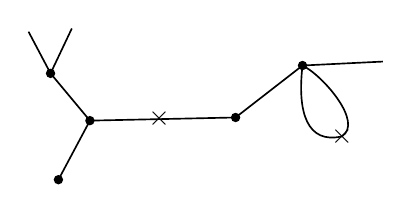
\begin{tikzpicture}[x=1cm,y=1cm,line width=.6pt]
\coordinate (a) at (0,0); \coordinate (b) at (-.5,.6); \coordinate (c) at (-.4,-.75); \coordinate (d) at (1.85,.04); \coordinate (e) at (2.7,.7);
\draw (b)--(a)--(c) (a)--(d)--(e);
\draw (b)--(-.78,1.13) (b)--(-.23,1.17) (e)--(3.72,.75);
\draw (e) .. controls (2.63,.1) and (2.76,-.3) .. (3.2,-.2) .. controls (3.48,-.02) and (2.95,.58) .. (e);
\foreach \p in {a,b,c,d,e} {\fill (\p) circle (1.7pt);}
\node at (.88,.02) {$\times$}; \node at (3.2,-.2) {$\times$};
\end{tikzpicture}}
donne
\figure{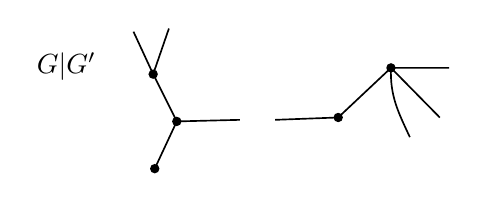
\begin{tikzpicture}[x=1cm,y=1cm,line width=.6pt]
\node[left] at (-.9,.7) {$\unsure{G|G'}$};
\coordinate (a) at (0,0); \coordinate (b) at (-.3,.6); \coordinate (c) at (-.28,-.6); \coordinate (d) at (2.05,.05); \coordinate (e) at (2.72,.68);
\draw (b)--(a)--(c) (a)--(.8,.02) (b)--(-.55,1.14) (b)--(-.1,1.18);
\draw (1.25,.02)--(d)--(e) (e)--(3.46,.68) (e)--(3.34,.05) (e) to[out=-92,in=115] (2.96,-.2);
\foreach \p in {a,b,c,d,e} {\fill (\p) circle (1.7pt);}
\end{tikzpicture}}
On trouve un nouveau graphe à branches orphelines (qui a des chances d'être disconnexe, même si $G$ était connexe \unsure{!|\}} — et si $G$ n'avait pas de branches flottantes, il a tendance à en avoir\ldots).
\margin{En sens inverse, $G$ se déduit de $G'$ en se donnant une involution ss pts fixes dans l'ens de ses branches ``flottantes'', ce qui permet de ``recoller'' celles-ci par leurs bouts.}
Si de plus on \deleted{\unsure{f}} remplace $G'$ par un sous-graphe déduit de $G'$ en enlevant certaines branches orphelines, et en prenant une réunion de composantes connexes de ce qui reste (en \deleted{\unsure{préservant}} \inserted{\unsure{outre|oubliant}}) c'est
\margin{97}
\scanpage{99}
kif-kif, car les composantes connexes ne changent pas en ajoutant ou retranchant des branches orphelines), on trouve la relation la plus générale entre $G$ et un $G'_0$, du type explicité dans la définition des ``morphismes de normalisation de m.graphes''.

On définit de façon évidente les composés de morphismes de normalisation. Le composé de morphismes de normalisation strict est strict. Les m.graphes avec morphismes de normalisation strict font une catégorie, dont les iso. sont les iso. ordinaires de m.graphes. Les morphismes de cette catégorie sont des monomorphismes. Quand on se borne aux morphismes \inserted{de norm.} stricts, on voit que (comme pour les morphismes de générisation) l'ens des sous-m.graphes stricts d'un m.graphe \inserted{$G$} est un ens. ordonné \deleted{\unsure{iso}}\inserted{anti}morphe à l'ens des parties de $A(G)$, en associant à tte partie $C\subset A(G$
\margin{98}
\scanpage{100}
\mspage{49}
la ``\uline{découpe}'' de $G$ suivant $C$, obtenue en ``coupant'' comme il a été dit \unsure{les} les milieux des arêtes $\in C$ (ce qui revient à ``enlever'' les arêtes, et à remplacer les côtés correspondants par des pts marqués).

Soit un morphisme de normalisation entre m.graphes
\[
(130)\qquad G'\longrightarrow G\deleted{\unsure{'}}.
\]
Si c'est un morphisme de normalisation \uline{strict}, on voit que $G'$ est stable ssi $G$ l'est. (Dans le cas général, on voit que si $S'\unsure{-|\longrightarrow}S$ est surjectif, et si $G'$ est stable, $G$ l'est aussi.)

\deleted{\unsure{Supp.}} Si $X$ est une courbe spéciale (sur une base quelconque $S$), épinglée par $G$, alors on voit (en procédant comme au début de la section) qu'on lui associe canoniquement une courbe spéciale $G'$-épinglée, d'où un foncteur
\[
(\unsure{130|131})\qquad M_G(S)\longrightarrow M_{G'}(S),
\]
\margin{99}
\scanpage{101}
qui pour $S$ variable est compatible aux chgts de base, et donne donc un morphisme des multiplicités modulaires \inserted{(si $G,G'$ sont stables)}
\[
(132)\qquad M_G\longrightarrow M_{G'},
\]
avec fonctorialité évidente pour les composés. Ainsi $M_G$ est un \uline{foncteur contravariant en} $G$ pour les morphismes de normalisation \inserted{de m.graphes stables}. Cette fois, on a

\uline{Proposition} a) Si $G\longrightarrow G'$ est un morphisme de normalisation \uline{strict}, alors (132) est un \uline{iso.} des multiplicités

b) Soient $G_\alpha$ des \deleted{\unsure{graphes connexes}}\inserted{m.graphes stables} \deleted{de} $G$ le m.graphe somme des $G_\alpha$. Alors le morphisme
\[
(133)\qquad M_G\longrightarrow\prod_\alpha M_{G_\alpha}
\]
est un iso. des multiplicités.
\margin{\uline{NB} On remplace la notation $\Pi M_G$ par $\Pi_1M_G$, pour ne pas confondre $\unsure{\Pi|\Pi_1}\deleted{\unsure{\Pi}}$ avec le signe du produit.}

\uline{Cor} $\Pi_1M_G$ est un foncteur contravariant en \deleted{\unsure{le}} m.graphe stable $G$ \deleted{\unsure{f}} pour les
\margin{100}
\scanpage{102}
\mspage{50}
morphismes de normalisation — il transforme morph. de norm. stricts en \deleted{isomorphismes}\inserted{équivalences} de \deleted{\unsure{multi}}groupoïdes, et sommes de m.graphes stables en produit des groupoïdes correspondants.

Pour nous, l'intérêt principal est dans la formule (obtenue en prenant le ``sous-objet strict'' minimal de $G$)
\[
(144)\qquad \Pi_1M_G\unsure{\simeq|\cong}\prod_{\alpha\in S}\Pi_1M_{\unsure{(g_\alpha,\widehat I_\alpha)|(G_\alpha,\widehat I_\alpha)}}\deleted{\unsure{*}}
\]
qui tient compte \inserted{de} et redonne automatiquement les \deleted{isomorphismes}\inserted{équivalences} des $\Pi M_{G'}\longrightarrow\Pi M_G$ par des morphismes de norm. stricts (qui induisent en effet des iso. pour les normalisés stricts $\widetilde G'$ et $\widetilde G$ de $G$,
\[
(145)\qquad
\diagram{\begin{tikzcd}[ampersand replacement=\&]
\widetilde G' \arrow[r] \arrow[d] \& \widetilde G \arrow[d] \\
G' \arrow[r] \& G
\end{tikzcd}}
\]
$G'\unsure{-|\longrightarrow}G$ est un morph. de norm. strict ssi le morphisme correspondant sur les normalisés (totaux) est un \uline{iso}\ldots)
\margin{101}
\scanpage{103}
Mais il faut encore expliciter la structure de $\unsure{S|\mathcal S}\Pi M_G$, en termes des $M_{g_\alpha,\widehat I_\alpha}$ — nous le ferons au n° suivant.

Pour un morphisme de normalisation quelconque (pas néc strict), le diagramme commutatif donne un diagramme comm (à iso. de foncteurs près)
\[
(146)\qquad
\diagram{\begin{tikzcd}[ampersand replacement=\&, column sep=small,row sep=large]
\Pi_1M_{\deleted{\unsure{G'}}G} \arrow[rr,leftrightarrow] \arrow[d,"\unsure{\sim|\wr}"] \&\& \Pi_1M_{G'} \arrow[d,"\unsure{\sim|\wr}"] \\
\Pi_1M_{\widetilde G}=\prod_{\alpha\in S}M_{g_\alpha,\widehat I_\alpha}
\arrow[rr] \arrow[dr,"{\substack{\text{on identifie }S'\\\text{à une partie de }S,\\\text{et }g_\alpha\text{ à }g'_{\alpha'}}}"'] \&\&
\Pi_1M_{\widetilde G'}=\prod_{\alpha'\in S'}\deleted{\unsure{1}}M_{g'_{\alpha'},\widehat I'_{\alpha'}} \\
\& \prod_{\alpha'\in S'\deleted{\unsure{*}}}M_{g_\alpha,\widehat I_\alpha} \arrow[ur,"\psi"'] \&
\end{tikzcd}}
\]
\margin{Ceci provient d'un diagramme analogue au niveau des multiplicités modulaires elles-mêmes\ldots}

La flèche oblique $\psi$ est induite par des flèches
\[
(147)\qquad \Pi_1M_{g_\alpha,\widehat I_\alpha}\longrightarrow\Pi_1M_{g_\alpha^{\deleted{\unsure{'}}},\widehat I'_\alpha}
\]
compte tenu du fait qu'on a $\widehat I'_\alpha\subset\widehat I_\alpha$.

Ainsi la connaissance des morphismes de normalisation \inserted{\unsure{généraux|général}} est \unsure{réduite|réduit} à celle des morphismes
\[
(148)\qquad \Pi_1M_{g,I}\longrightarrow\Pi_1M_{g,I'}\quad\text{pour }I'\subset I,
\]
\margin{102}
\scanpage{104}
\mspage{51}
qui sont induits par les morphismes de normalisation entre m.graphes associés aux graphes monoponctuels. Bien entendu, pour pouvoir reconstituer bel et bien les \inserted{effets \deleted{\unsure{sur}} en $\Pi_1M$ des} morphismes de normalisation, et leurs propriétés de commutation aux iso., il faut utiliser les \deleted{\unsure{covariances}} \unsure{commutation|covariances} de (148) à
\[
\unsure{\mathfrak S|\mathcal S}_{I,I'}\simeq\unsure{\mathfrak S|\mathcal S}_{I'}\times\unsure{\mathfrak S|\mathcal S}_{I\setminus I'}\qquad\ldots
\]

\uline{Programme} Déterminer (à équivalence ``canonique'' près) tous les groupoïdes $\Pi_1M_{g,I}$, avec leur dépendance fonctorielle pour \inserted{$g$ fixe,} $I$ variable (des mono. $I'\hookrightarrow I$) via les morphismes de normalisation (148).
\margin{par ``\unsure{gén.|génér.} et relations'' — \unsure{définies|définis} en termes purement algébriques\ldots}

De plus, pour tt MD-graphe $G$, déterminer l'extension $S\Pi_1M_G$ de
\[
\Pi_1M_G\simeq\prod_{\alpha\in S(G)}\Pi_1M_{\unsure{\alpha|g_\alpha},\widehat I_\alpha}\quad\text{par }\mathbb Z^{\widetilde A(G)},
\]
et pour un morphisme de générisation (p.ex. un iso!) \deleted{donné} $G\longrightarrow G'$ de MD-graphes, \deleted{définir}\inserted{déterminer} le morphisme de groupoïdes de générisation correspondant
\[
S\Pi_1M_G\longrightarrow S\Pi_1M_{G'}.
\]
\margin{\figure{
\begin{tikzpicture}\draw (0,0)--(.05,-8);\end{tikzpicture}}}
\margin{103}
\scanpage{105}
12) \uline{Relation entre les morphismes de générisation et morphismes de normalisation}

\deleted{Avant d'aborder une réalisation \unsure{calculatoire} de ce programme, j'ai envie d'examiner les relations entre les deux types de morphismes sur les $\Pi_1M_G$, $S\Pi_1M_G$ — \deleted{\unsure{les cas où les}}\inserted{\unsure{au delà de}} de la constatation $\pm$ triviale que pour des isomorphismes de graphes, les deux sont ``compatibles'' avec les projections $S\Pi_1M_G\longrightarrow\Pi_1M_G$. Pour le dire autrement, j'ai envie, pour une inclusion \uline{stricte} $I'\subset I$, d'examiner ``l'effet à l'infini'' des morphismes de groupoïdes (148).

Soit donc $G_{g,I}$ le \inserted{MD-}graphe réduit à un seul sommet de genre $g$, et avec $I$ comme ens de pts marqués. Soit $G$ un graphe de type numérique $(g,\nu=\operatorname{card} I)$, et considérons un morphisme de générisation
\[
(149)\qquad G\longrightarrow G_{g,I}\qquad\text{i.e. un iso. }I(G)\simeq I
\]
d'où un \deleted{diag.}\unsure{germe|gramme} de multiplicités
\margin{\deleted{$\unsure{M_G^*}$}}
\[
(150)\quad
\diagram{\begin{tikzcd}[ampersand replacement=\&, column sep=large,row sep=small]
M^*_{G,G_{g,I}} \arrow[r,leftrightarrow] \arrow[dr] \& (M_{G,G_{g,I}},\Gamma'_G) \& \\
\& M_{g,I} \& (M_G,\Gamma'_G)\arrow[ul,"\simeq"']
\end{tikzcd}}
\]
}
\margin{104}
\scanpage{106}
\mspage{52}
11) Digression : déploiement d'un diviseur à croisements normaux.

Pour fixer les idées, je vais me placer dans le contexte des multiplicités analytiques lisses — mais on pourrait aussi, en prenant des multiplicités analytiques lisses \uline{relatives} — ou en remplaçant \unsure{l'hyp.} \unsure{analytiques|analytique} par des hyp. topologiques ad-hoc — ou en passant au contexte schématique\ldots.

Soit $X$ une multiplicité analytique lisse, et $D$ un diviseur sur $X$ à croisements normaux (hyp. purement locale en $(X,D)$, par définition). \deleted{Soit \unsure{$G$} un}

Pour tout pt $x$ de $D$, l'ens des ``branches'' de $D$ passant par $x$ est un ensemble fini $I(x)$, Par définition, les \uline{germes \inserted{en $x$} de sous-multiplicités} \uuline{\unsure{attachés|attachées}} \uuline{à $D$} sont les intersections d'un \unsure{nb|ens} fini \deleted{de} parmi les $D_{x,i}\in I(x)$.
\margin{il vaut mieux prendre un $x\in X$, et poser $I(x)=\varnothing$ si $x\notin D$}
Ces germes forment un ensemble ordonné \inserted{$\Delta_x\unsure{(=\Delta_x(X,D))}$} antiisomorphe à $\mathcal P(I(x))$, \deleted{Si \unsure{$J$ est}}\inserted{la codimension} \deleted{\unsure{une}} de $D_{x,J}$ $(J\subset I(x))$ étant donnée par
\[
(149)\qquad \operatorname{codim}(D_{x,J},X_x)=\operatorname{card}J
\]
\margin{105}
\scanpage{107}
Soit $J$ un ensemble ordonné, on s'intéresse aux plongements d'ensembles ordonnés
\[
(150)\qquad J\mathrel{\overset{\varphi}{\hookrightarrow}}\Delta_x\unsure{\xi}\simeq\mathcal P(I(x))^\circ
\]
Un tel plongement donne une ``fonction codimension'' sur $J$, en composant, \inserted{soit $d$,} et \deleted{dire que $\varphi$ est un plongement d'ens. ordonnés signifie que}\inserted{on suppose donné déjà $d$ d'avance sur $J$} satisfaisant
\[
(151)\qquad\text{Si }x<y\quad\text{on a}\quad\unsure{d|c}(x)<c(y),
\]
et on se borne aux $\varphi$ qui sont des \unsure{plongts|plongements} ordonnés, compatibles avec \unsure{foncts} codim sur $J$ et sur $\Delta_x$.
\deleted{On suppose de plus que $J$ a un plus petit élément (ce qui correspond donc à une codim. maximale \deleted{qui est} soit $d(J)$) — quitte à le rajouter, s'il n'y est déjà!}

Considérons, \inserted{pour tout $\unsure{q|d}\in\mathbb N^*$,} la multiplicité analytique formée des couples $(x,\unsure{V})$, où $x$ est un pt de $D$ et $V$ un germe de sous-multiplicité de $X$ attaché à $D$, de codim $\unsure{q|d}$. On \deleted{voit} voit aisément que ce sont \inserted{bien} là les points d'une multiplicité analytique que je note $D_{\unsure{q|d}}$, et on a un morphisme
\margin{106}
\scanpage{108}
\mspage{53}
canonique
\[
(152)\qquad D_{\unsure{q|d}}\longrightarrow X
\]
\margin{On introduit aussi $D_0=X$, et $D_0\longrightarrow X$ l'identité}
qui se factorise d'ailleurs par $D$, et qui est un morphisme d'immersion local, de codim $q$. \unsure{Sur|Pour} $D_{\unsure{q|d}}$, on a un \unsure{revêtt|revêtement} étale à $q$ feuillets, noté $\overset{\deleted{\unsure{q}}}{\widetilde D_{\unsure{q|d}}}$, \deleted{formé des couples}\inserted{dont la fibre en} un pt $(x,V)$ est \unsure{formée|formé} de l'ens des $\unsure{q|d}$ branches $D_{xi}$ de $D$ en $x$ qui contiennent $V$. Donc les \deleted{\unsure{points|couples}} pts de $\widetilde D_{\unsure{q|d}}$ correspondent aux triplets $(x,\unsure{V},W)$, où $x$ est un pt de $D$, et $V\subset W$ des germes de ss-multiplicités de $X$ en $x$ attachées à $D$, de codims respectives $\unsure{q|d}$ et $1$. On trouve donc un morphisme canonique
\[
\diagram{\begin{tikzcd}[ampersand replacement=\&, row sep=small]
\widetilde D_{\unsure{q|d}}\arrow[r] \& D_1\\
(x,V,W)\arrow[r,mapsto] \& W
\end{tikzcd}}
\]

Plus généralement, si $J$ est un ens. fini ordonné comme ci-dessus, \inserted{muni d'une fonction codim,} on \deleted{\unsure{en}} désigne par $D_J$ la \deleted{\unsure{var.}} multiplicité \deleted{formée}\inserted{dont} les points sont les couples d'un $x\in\deleted{D}\inserted{X}$ \inserted{de codim $d=d(J)$,} et d'un \unsure{plongt|plongement} d'ens. ordonnés, compatible \deleted{\unsure{avec|aux}} fonctions codim
\margin{on suppose la fonction codim strictement décr. cf (151)}
\[
(152)\qquad J\mathrel{\overset{\varphi}{\hookrightarrow}}\Delta_x\simeq\mathcal P(I(x))^\circ
\]
\margin{107}
\scanpage{109}
\deleted{On va \deleted{\unsure{désormais|d'ailleurs}} supposer que $J$ a un plus petit élément $e_J$, et $d(J)=d$ sa codim.}

Alors la multiplicité $D_J$ est lisse, \deleted{de} et le morphisme canonique
\[
(153)\qquad D_J\longrightarrow X
\]
est une imm. \unsure{locale|local} de codim $d$.
Elle se factorise par $D$, sauf dans le cas où $d(I)$\inserted{$=0$ i.e. $I$} est réduit à un seul élément, de codim. nulle, auquel cas $D_J=\deleted{D_0}=X$.

Si $J$ est formé d'un seul élément, de codim $d$, on retrouve $D_d$; S'il est formé de deux éléments, \deleted{le plus} $e_J$ de codim $d$ et $e'$ de codim $1$, on retrouve $\widetilde D_d$.

Si $J$ est de dim totale $d=d(J)$, \unsure{on peut} \deleted{\unsure{retrouver}} reconstituer $D_J$ à \unsure{l'aide de} $D_d$ et de $\widetilde D_d$, via le \unsure{revêtement} principal (torseur sous $\unsure{\mathfrak S|\mathcal S}_d$) \unsure{sur} $D_d$ associé à $\widetilde D_d$, soit $\overset{\deleted{\unsure{\sim}}}{D'_d}$, qui s'identifie aussi à $D_{\mathbf I(d)}$, où $\mathbf I(d)$ l'ens ordonné
\diagram{\begin{tikzcd}[ampersand replacement=\&, column sep=small]
\underset{d}{\bullet}\arrow[r,dash]\&\underset{d-1}{\bullet}\arrow[r,dash]\&\underset{\unsure{2}}{\bullet}\arrow[r,dash]\&\underset{1}{\bullet}\arrow[r,dash]\&\underset{0}{\bullet}
\end{tikzcd}}
(degré maximal de codim $d$). En effet, considérons
\margin{Mais l'expression de $\overset{\deleted{\unsure{\sim}}}{D'_d}$ comme $D_{I_d}$ \unsure{ne met pas en évidence les opérations de|ne vaut pas une évidence, car opération de} $\unsure{\mathfrak S|\mathcal S}_d$ \unsure{sur} $\widetilde D_d$ — \unsure{pour ceci}; il faut \unsure{prendre} \illegible{2} l'ens ordonné $\unsure{K}_d$, \unsure{ayant} un \deleted{\unsure{élément}} plus petit élément de codim $d$, et $d$ éléments de codim $1$\ldots}
\margin{les \unsure{entiers} sont les \unsure{sommets identifiés par} leur codim.}
\margin{108}
\scanpage{110}
\mspage{54}
l'ensemble fini
\[
\begin{aligned}
(154)\quad H(J)={}&\text{ensemble des plongements d'ens. ordonnés, compatibles avec}\\
&\text{les \unsure{f} codim, de }J\text{ dans }\deleted{\mathcal P([1,n]\cap\mathbb N)}\mathcal P(I_d)^\circ\\
&\text{(où }I_d\overset{\mathrm{def}}=[1,d]\cap\mathbb N\text{)}
\end{aligned}
\]
alors $\unsure{\mathfrak S|\mathcal S}_d$ opère à gauche sur $H(J)$, et on a un iso. can. de $D$-multiplicités
\[
(155)\qquad D_J\simeq\unsure{\widetilde D'_d|\widetilde{\widetilde D}_d}\mathbin{\unsure{\wedge|\times}}_{(\unsure{\mathfrak S|\mathcal S}_d)_{D_d}}H(J).
\]

Soient \deleted{$J$} $(J,\underline{\unsure{c|d}})$ et $(J',\underline{c}')$ deux ens. ordonnés finis munis de fonctions codim, et
\[
(156)\qquad J'\mathrel{\overset{f}{\hookrightarrow}}J\deleted{\unsure{'}}
\]
un \unsure{plongt|plongement} d'ens ordonnés, compatible aux fonctions codim, on trouve alors un \deleted{application} morphisme canonique
\[
(157)\qquad D_{J\deleted{\unsure{'}}}\longrightarrow D_{J'},
\]
je me demande \deleted{\unsure{sous forme}}\inserted{en termes} de quelles données suppl. \inserted{(si besoin est)} sur les $(D_d,\unsure{\widetilde D'_{d'}|\widetilde D'_d})$ on peut reconstituer cette dépendance fonctorielle de $D_J$ \unsure{p.r.|p.v.} à $J$, via (155). \deleted{Considérons}\inserted{Comme la} \deleted{d'abord le plus petit élément $e_J$, de $c$} dépendance fonctorielle en $J$ pour les \uline{iso}
\margin{109}
\scanpage{111}
est \unsure{claire|clair} sur l'expression 155, \deleted{\unsure{les}} $J'\subset J$, Considérons \deleted{le plus petit}\inserted{un} élément \deleted{$e_{J'}$}\inserted{$x$} de $J'$, \inserted{$\ne e_J$} \deleted{qui} est de codim $\delta$ \inserted{($\unsure{\le|\ne}d$)} et considérons \inserted{d'abord} le composé
\[
(158)\quad
\diagram{\begin{tikzcd}[ampersand replacement=\&, column sep=large,row sep=small]
D_J\arrow[r]\arrow[dr,draw=none,"{\deleted{\searrow}}" description]\&D_{J'}\arrow[r,"f_x"]\&D_\delta\\
\&\deleted{D_{d,\delta}}\arrow[ur,draw=none,"{\deleted{\nearrow\,\unsure{\mathrm{can.}}}}" description]\&
\end{tikzcd}}
\]
\margin{\inserted{$f_x$ défini par fonctorialité par l'inclusion $\{x\}\subset J'$}}
on va le mettre en relation avec l'hom.
\[
(159)\qquad D_J\longrightarrow D_{d,\delta}
\]
suivant (où $D_{d,\delta}=D_{\Delta(d,\delta)}$, $\Delta(d,\delta)$ étant le drapeau \deleted{type} de type $d,\delta$, i.e. l'ens. ordonné \deleted{avec} fonction codim
\diagram{\begin{tikzcd}[ampersand replacement=\&, column sep=small]\underset{d}{\bullet}\arrow[r,dash]\&\underset{\delta}{\bullet}\end{tikzcd}}
(si $\delta<d$!) \deleted{\unsure{resp.} \diagram{\begin{tikzcd}\underset{d=\delta}{\bullet}\end{tikzcd}}}
\deleted{(\unsure{si|et} $\delta=1$)}, on a, en appliquant (155) au cas de $\inserted{J=}\Delta(d,\delta)$, \deleted{au lieu de} \deleted{\unsure{l'}} l'isom canonique
\[
(160)\qquad D_{d,\delta}\simeq\unsure{\widetilde D'_d|\widetilde{\widetilde D}_d}\mathbin{\unsure{\wedge|\times}}_{(\unsure{\mathfrak S|\mathcal S}_d)_{D_d}}\mathcal P_\delta(I_{\inserted{d}}\deleted{(d)})
\]
D'autre part, on a (avec la notation (154) pour $H(J)$), \deleted{pour} l'élément $\unsure{x}\in J$ fixé de $J$, \inserted{\unsure{de codim} $d'=\operatorname{cod}(e')$,} une application
\[
(161)\quad\diagram{\begin{tikzcd}[ampersand replacement=\&, row sep=small]
H(J)\arrow[r]\&\mathcal P_\delta(I_d)\\
h\arrow[r,mapsto]\&h(\unsure{x})
\end{tikzcd}}
\]
\margin{110}
\scanpage{112}
\mspage{55}
compatible avec les opérations de $\unsure{\mathfrak S|\mathcal S}_d$, d'où un morphisme
\[
(162)\quad\diagram{\begin{tikzcd}[ampersand replacement=\&, column sep=large,row sep=small]
D_J\arrow[r,"f_x"]\arrow[d,phantom,"\wr" description]\&D_{d,\delta}\deleted{\unsure{'}}\arrow[d,phantom,"\wr" description]\\
\widetilde D_d\wedge_{\unsure{\mathfrak S|\mathcal S}_d}H(J)\&\unsure{\widetilde D'_d|\widetilde{\widetilde D}_d}\wedge_{\unsure{\mathfrak S|\mathcal S}_d}\mathcal P_\delta(I_d)
\end{tikzcd}}
\]
\deleted{Ceci posé, il} Cette application est décrite entièrement en termes du rev. principal $\widetilde D_d$ de $D_d$, de groupe $\unsure{\mathfrak S|\mathcal S}_d$, \inserted{et de $x\in J$.} On a d'autre part, par ``fonctorialité \inserted{en $J$ de $D_J$}'', les \deleted{morphismes}\inserted{diagrammes} commutatifs étendant (158)
\[
\deleted{(\unsure{162})\qquad D_{d,\unsure{d'|\delta}}\longrightarrow D_{d'}}
\]
\deleted{et on a}
\[
(163)\quad\diagram{\begin{tikzcd}[ampersand replacement=\&]
D_J\arrow[r]\arrow[d]\&D_{J'}\arrow[d,"f_x"]\\
D_{d,\delta}\arrow[r]\&D_\delta
\end{tikzcd}},
\]
où $D_J-D_{d,\delta}$ et $D_{d,\delta}-D_\delta$ sont définis par fonctorialité par les inclusions $\deleted{\unsure{\{e\}}}\{x\}\subset\{x,e\}\subset J$. On \deleted{Cela signifie}\inserted{\unsure{peut voir aussitôt}} que $D_J\unsure{-|\to}D_{d,\delta}$ est décrit par la \unsure{nôtre|flèche} (162), donc le composé (158) est connu quand on connaît les $D_{d,\delta}\longrightarrow D_\delta$
\margin{111}
\scanpage{113}
-- et quand les composés (158) sont connus, on vérifie que les morphismes $D_J-D_{J'}$ sont connus,\ldots

On est donc intéressé plus particulièrement par les hom
\[
(164)\qquad D_{d,\delta}\unsure{-|\longrightarrow}D_\delta\qquad(d>\delta)
\]
qui jouent le rôle des ``morphismes but'' alors que les $D_{d,\delta}-D_d$ jouent le rôle des ``morphismes source'', et $D_{d,\delta}$ le rôle de ``\deleted{\unsure{f}}multiplicité des flèches'' (\unsure{ou|où} mor. d'inclusion) -- entre éléments de sous-multiplicités \inserted{de $X$} associés à $D$.

On a des isom. can.
\[
(165)\qquad D_{d,d'}\times_{D_{d'}}D_{d',d''}\simeq D_{d,d',d''}\qquad\text{si }d>d'>d''
\]
et on \deleted{\unsure{en}} déduit de cette description les morphismes canoniques
\diagram{
\begin{tikzcd}[ampersand replacement=\&, column sep=large,row sep=small]
\& \& D_d\\
\& D_{d,d'}\arrow[ur]\arrow[dr] \&\\
D_{d,d',d''}\arrow[ur]\arrow[dr,dash] \& \& D_{d'}\\
\& D_{d',d''}\arrow[ur]\arrow[dr] \&\\
\& \& D_{d''}
\end{tikzcd}
\qquad(166)
}
mais non directement \deleted{$\unsure{D_{d'}}$}
\[
(167)\qquad D_{d,d',d''}\longrightarrow D_{d,d''},
\]
mais on note que
\[
(168)\qquad D_{d,d''}\unsure{-|\longrightarrow}D_d\times D_{d''}.
\]
\margin{112}
\scanpage{114}
\mspage{56}
\margin{ceci marche au moins dans la Cat des espaces analytiques}
est un mono $\leftarrow$, et (167) est déterminé par la condition que son composé avec (168) est donné par les morphismes
\diagram{\begin{tikzcd}[ampersand replacement=\&, column sep=large,row sep=small]
\& D_d\\
D_{d,d',d''}\arrow[ur]\arrow[dr] \&\\
\& D_{d''}
\end{tikzcd}}
qui figurent dans (\unsure{166}).

\margin{on pourrait l'appeler aussi ``\uline{structure de drapeaux} analytiques''}
Une ``\uline{Structure de déploiement d'\unsure{intersection} normale}'' se définit \inserted{d'abord} comme une structure de ``catégorie \deleted{multiplicité} analytique'' $\mathcal D$, i.e. d'une catégorie dans la catégorie des espaces analytiques
\margin{(d'abord \unsure{$\mathcal E$} dans la cat des \uline{espaces} \unsure{analytiques})}
\diagram{
(169)\quad\left\{\begin{array}{ll}
D_* & \text{espace analytique des objets}\\[5pt]
D_{**} & \text{\rule{4cm}{0.3pt}\quad flèches}\\[8pt]
\begin{tikzcd}[ampersand replacement=\&,row sep=small,column sep=small,baseline=(current bounding box.center)]
\& D_{**}\arrow[dl,"\unsure{\sigma|s}"']\arrow[dr,"b"]\&\\
D_*\&\&D_*
\end{tikzcd}
&\text{morphismes ``source'' et ``but''}\\[8pt]
D_*\longrightarrow D_{**} & \text{morphisme ``\unsure{identique}''}\\[8pt]
\multicolumn{2}{l}{(D_{**},b)\times_{D_*}(D_{**},\unsure{\sigma|s})\longrightarrow D_{**}}\\[5pt]
\multicolumn{2}{c}{(u,v)\longmapsto v\circ u}\\[5pt]
\multicolumn{2}{l}{\text{(morphisme ``composition des flèches'')}}
\end{array}\right.
}
\deleted{Et} Ces données satisfont aux axiomes habituels (associativité, unité\ldots) exprimant que
\margin{113}
\scanpage{115}
pour $\forall S$, \unsure{les|le} \deleted{\unsure{ens}} ``p\textsuperscript{ts} de $S$ à \unsure{valeur|valeurs} dans $\mathcal D$ (formé de $D_*(S)$, $D_{**}(S)$ etc) est une catégorie. On suppose de plus donnée une fonction ``codimension'' sur $D_*$
\[
(170)\qquad D_*\xrightarrow{c}\mathbb N
\]
\margin{c'est inutile, elle sort des autres structures, cf plus bas\ldots}
ce qui revient à une décomposition
\[
(\unsure{271|171})\qquad D_*=\coprod_{d\in\mathbb N}D_d
\]
d'où une décomposition correspondante
\[
(172)\qquad D_{**}=\coprod_{d,d'\in\mathbb N\times\mathbb N}D_{d,d'}
\]
où
\[
(173)\qquad\begin{gathered}
D_{d,d'}=\text{im. inverse de }D_d\times D_{d'}\\
\text{par }D_{*,*}\xrightarrow{(\unsure{\sigma|s},b)}D_*\times D_*.
\end{gathered}
\]

On fait les hypothèses suivantes
\diagram{
(174)\quad\left\{\begin{array}{l}
\text{a) }D_{d,d'}=\varnothing\text{ si }d'>d\quad\text{(le but est de codim}\\
\hfill\leq\text{ la codim de la source)}\\[8pt]
\text{b) le morphisme ``identité'' }D_*\longrightarrow D_{**}\quad\deleted{\text{\unsure{induit}}}\\
\quad\text{(qui se factorise en }\coprod_{d\in\mathbb N}D_d\longrightarrow\coprod_{\unsure{d\in\mathbb N}}D_{d,d}\text{) induit}\\
\quad\text{des iso}\qquad D_d\simeq D_{d,d}\\
\quad\text{(une flèche dont source et but sont de }=\text{ codim,}\\
\hfill\Rightarrow\text{ une identité)}\\[8pt]
\text{c) Pour }d\in\mathbb N\text{ fixé, le morphisme ``source'' }\deleted{\underset{\unsure{\prod d'|\coprod d'}}{D_{d,*}}\xrightarrow{\unsure{b_*}}D_*}
\end{array}\right.
}
\margin{ceci conséquence de c) ci-dessous (\unsure{trop fort?|thm prouvé?})}
\margin{114}
\scanpage{116}
\mspage{57}
\margin{(174)\quad $\left\{\rule{0pt}{14em}\right.$}
\diagram{\begin{tikzcd}[ampersand replacement=\&, column sep=large,row sep=small]
D_{d,*} \arrow[r,"\sigma_d"] \arrow[d,equal,"\mathrm{def}"'] \& D_d \\
\displaystyle\coprod_{\substack{\deleted{\unsure{d'}}\\d'\in\mathbb N}}D_{d,d'}=\sigma^{-1}(D_d) \&
\end{tikzcd}}
qui fait de $D_{d,*}$ un esp. analytique sur $D_d$, \deleted{\unsure{prédisposé}} relativement ordonné (par la relation de factorisabilité
\diagram{\begin{tikzcd}[ampersand replacement=\&, column sep=small,row sep=small]
{} \& {} \arrow[dd,dotted] \\
\bullet \arrow[ru] \arrow[rd] \& \\
{} \& {}
\end{tikzcd}}
des flèches de source donnée) et loc. isomorphe à $\deleted{\unsure{E}}\unsure{\mathcal P}(I_d)^{\deleted{\unsure{0}}}_{D_d}$ \inserted{``pondéré'' par $d'$, avec sa relation d'ordre et la fonction ``cardinal''} (--- le faisceau constant d'ensembles ordonnés \unsure{simpliciaux} $\mathcal P(I_d)^0$ ---

Cela redonne donc un rev. $D'_d$ principal de groupe $\unsure{G_d|\mathfrak S_d}$, permettant de reconstituer les $D_{d,d'}$ --- mais pour reconstituer $D$, il faut de plus se donner \deleted{\unsure{les}} au moins les $D_{d,d'}\unsure{\text{---}|\longrightarrow}D_{d'}$, et (c'est plus sûr!) aussi
\[
D_{\unsure{d|d^\circ},d'}\mathbin{\times}_{D_{d'}}D_{d',d''}\unsure{\text{---}|\longrightarrow}D_{\unsure{d|d^\circ},d''}
\]
(la flèche composition), car il n'est pas clair, avec les seules hyp. faites jusqu'à présent, que les morphismes
\[
D_{d,d''}\unsure{\text{---}|\longrightarrow}D_d\times D_{d''}
\]
sont mono ?, i.e. que ``les flèches sont déterminées par sa source et par son but''. Mais finalement si, c'est une conséquence de c). Donc
\margin{115}
\scanpage{117}
la structure envisagée peut se décrire par

 a) famille d'espaces analytiques $(D_d)_{d\in\mathbb N^{\deleted{\unsure{*}}}}$

 b) $\forall\,d\in\mathbb N$, un revêtement principal \inserted{$D'_d$} de $D_d$, de groupe $\unsure{\mathfrak S_d|G_d}$ --- d'où des $D_{d,d'}$ $(0\leq d'\leq d)$

\margin{\unsure{on aura} $D_{d,d}\simeq D_{d,0}\simeq D_d$\par $D_{d,1}$ est le rev. à $d$ feuillets de $D_d$ qui correspond à $D'_d$.}

 c) des morphismes
\[
D_{d,d'}\xrightarrow{b}D_{d'}\qquad(\text{pour }0\leq d'\unsure{<|\leq}\unsure{d|d''}),
\]
et en plus des diagrammes cartésiens

\deleted{avec la condition que les morphismes can. (pour $d\geq d'\geq d''$)}
\[
\deleted{D_{d,d',d''}\overset{\mathrm{def}}{=}D_{d,d'}\mathbin\times_{D_{d'}}D_{d',d''}\longrightarrow D_d\mathbin\times D_{d''}}
\]
\deleted{d) $D_{d,d'}\mathbin\times_{D_{d'}}D'_{d'}\unsure{\sim|\simeq}$}
\deleted{d) $\unsure{D'_{d'}|D'_{d,d'}}$}
\deleted{$\unsure{B_{d,d'}|D_{d,d'}}$}

 d) \quad(175)
\diagram{\begin{tikzcd}[ampersand replacement=\&, column sep=large,row sep=large]
D'_{d,d'} \arrow[r,very thick] \arrow[d,"\mathrm{can}"'] \arrow[dr,phantom,"\uline{\mathrm{cart}}"] \& D'_{d'} \arrow[d,"\mathrm{can}"] \\
D_{d,d'} \arrow[r,"b"'] \& D_{d'}
\end{tikzcd}}
où $D'_{d,d'}$ est le revêtement $\unsure{\mathfrak S_{d'}|G_{d'}}$-principal de
\[
D_{d,d'}\simeq D'_d\mathbin\times_{(\unsure{\mathfrak S_d|G_d})_{D_d}}\mathcal P_{d'}(I_d),
\]
associé au $d'$-rev. ``tautologique'' de $D_{d,d'}$; ce qui donne, pour $D_{d,d',d''}$ déduit de ce rev. de $D_{d,d'}$ par
\[
D_{d,d',d''}\overset{\mathrm{def}}{=}D'_{d,d'}\mathbin\wedge_{(\unsure{\mathfrak S_{d'}|G_{d'}})_{D_{d,d'}}}\mathcal P_{d''}(I_{d'}),
\]
\margin{\uline{NB} $D_{d,d'}$ et $D_{d,d',d''}$ sont déduits directement de $D'_d$.}
un \deleted{\unsure{rev.}} diagramme cartésien

(176)\quad
\diagram{\begin{tikzcd}[ampersand replacement=\&, column sep=large,row sep=large]
D_{\unsure{d},d',d''}\arrow[r]\arrow[d]\arrow[dr,phantom,"\mathrm{cart}"] \& D_{d',d''}\arrow[d]\\
D_{d,d'}\arrow[r]\&D_{d'}
\end{tikzcd}}
\margin{116}
\scanpage{118}
\mspage{58}
et il faut demander de plus qu'on ait commutativité dans le \deleted{\unsure{simple}} diagramme

(177)\quad
\diagram{\begin{tikzcd}[ampersand replacement=\&, column sep=large,row sep=large]
D_{d,d',d''}\arrow[r]\arrow[d,"\mathrm{tautol.}"'] \& D_{d',d''}\arrow[d,"\text{``but''}"]\\
D_{d,d''}\arrow[r,"\text{``but''}"'] \& D_{d''}
\end{tikzcd}}.

\uline{Remarque} L'axiomatique précédente a un sens dans chaque site (\deleted{\unsure{ce qui}} le fait de travailler dans un site donne un sens à la notion de revêtement principal\ldots), où on suppose que les fonctions loc constantes définissent une décomposition en sommes disjointes d'un objet. Il est inutile en fait de se \uline{donner} la fonction codimension, elle est contenue dans la condition c), qui implique a) et b).

Pour faire le lien avec l'intuition ``croisements normaux'', on va faire de plus une hypothèse ad hoc sur la nature des morphismes
\[
D_{d,d'}\longrightarrow D_{d'}
\]
(NB $D_{d,d'}\longrightarrow D_d$ est un rev. fini étale\ldots), p.ex.
\margin{117}
\scanpage{119}
que c'est une \uline{immersion locale} d'espaces \uline{analytiques} lisses (ou lisses sur un esp. analytique donné, dans une situation relative\ldots);

\deleted{\inserted{de codimens. $d-d'$}}
\deleted{On doit faire l'hyp. de finité, que}
\deleted{Notons que pour que $D_{d,d'}\unsure{\text{---}|\longrightarrow}D_{d'}$ soit une imm. loc., il suffit que}
\[
\deleted{D_{d,0}\longrightarrow D_0\quad\text{et}\quad D_{d',0}\longrightarrow D_0}
\]
\diagram{\begin{tikzcd}[ampersand replacement=\&, column sep=large,row sep=small]
\deleted{D_{d,0}}\arrow[r]\arrow[d,equal]\&\deleted{D_0}\&\deleted{D_{d',0}}\arrow[r]\arrow[d,equal]\&\deleted{D_0}\\
\deleted{D_d}\&\&\deleted{D_{d'}}\&
\end{tikzcd}}
\deleted{le soient, comme on voit en considérant}
\diagram{\begin{tikzcd}[ampersand replacement=\&, column sep=large,row sep=large]
\&\deleted{D_{d,0}}\arrow[dr] \&\\
\deleted{D_{d,d',0}}\arrow[ur]\arrow[r]\arrow[d,"\deleted{\sim}"'] \& \deleted{D_{d',0}}\arrow[r]\arrow[d,"\deleted{\sim}"] \&\deleted{D_0}\\
\deleted{D_{d,d'}}\arrow[r,Rightarrow]\arrow[ur,phantom,"\deleted{\mathrm{cart}}"] \&\deleted{D_{d'}}\&
\end{tikzcd}}

Dans le cas lisse ou relativement lisse, l'hyp. d'imm. loc. équivaut d'ailleurs à celle de mono local, qui garde un sens dans tout site.

Notons que pour $\unsure{\forall|\mathrm{tt}}\,d$ on a

(178)\quad
\diagram{\begin{tikzcd}[ampersand replacement=\&, column sep=large,row sep=large]
D_{d,0}\arrow[d,"\sim"']\arrow[dr,no head]\&\\
D_d\&D_0\overset{\mathrm{def}}{=}X
\end{tikzcd}}
\margin{$D$ est une catég. dans la catégorie $(\mathrm{An})_{D_0}$.}
donc les $D_d$ s'envoient tous \unsure{can\textsuperscript{t}} dans $X=D_0$, et on aura commutativité dans

(179)\quad
\diagram{\begin{tikzcd}[ampersand replacement=\&, column sep=large,row sep=large]
D_{d,d'}\arrow[r,"b"]\arrow[d,"\sigma"']\&D_{d'}\arrow[d]\\
D_d\arrow[r]\&\deleted{\unsure{D_0}}\inserted{\unsure{X}}
\end{tikzcd}}
\margin{118}
\scanpage{120}
\mspage{59}
où $\sigma$ est un rev. étale donc un iso. local. Donc on voit que si $D_d\unsure{\text{---}|\longrightarrow}D_0$ et $D_{d'}\unsure{\text{---}|\longrightarrow}D_0$ sont des immersions locales (resp. des mono. locaux), il en est de $=$ de $D_{d,d'}\unsure{\text{---}|\longrightarrow}D_{d'}$. De plus, dans le cas lisse, on voit que la codim. de $D_{d,d'}\unsure{\text{---}|\longrightarrow}D_{d'}$ est égale à la diff. des codim de $D_d\unsure{\text{---}|\longrightarrow}D_0$ et $D_{d'}\unsure{\text{---}|\longrightarrow}D_0$. On supposera, bien sûr (dernier axiome ! (?))
\[
(180)\qquad D_d\unsure{\text{---}|\longrightarrow}D_0\quad\text{est de codim }d
\]

\deleted{\unsure{Et}} Et plus précisément encore ceci. Soit \deleted{\unsure{(181)}} $x\in D_d$, d'où $I(x)$ de cardinal $d$ (tel qu'on ait
\[
(181)\qquad(D'_d)_x\simeq\unsure{\mathcal P}(I_x)
\]
)
\deleted{qui} \deleted{considérons les} on a aussi
\[
(182)\qquad\begin{aligned}
I_x&=\text{germes de sections en }x\\
&\qquad\text{du rev. }D_{d,1}\text{ au dessus de }\unsure{D_d}\\
&\simeq(D_{d,1})_x,
\end{aligned}
\]
Considérons alors les composés $(i\in I)$
\diagram{\begin{tikzcd}[ampersand replacement=\&, column sep=large]
D_d\arrow[r,"s_i"]\&D_{d,1}\arrow[r,"\substack{\mathrm{can}\\\unsure{b|a}}"]\&\unsure{D_1|D_d}\deleted{\unsure{=D_d}}\arrow[r]\&X
\end{tikzcd}}
qui sont tous égaux au morph. can. $D_d\xrightarrow{\mathrm{id}}\deleted{\unsure{D_d}}$, d'autre part les \unsure{images} $x_i$ de $x$ dans $D_1$ pr. les $s_i$.
\margin{119}
\scanpage{121}
définissent des germes de sous-espaces \inserted{$D_x^i$} de $X$ en l'image $a$ de $x$ dans $X$, qui contiennent le germe défini par $(D_d,x)\longrightarrow(X,a)$. Ceci dit, on veut que ce dernier germe soit l'\uline{intersection} des germes $D_x^i$, \inserted{et} \unsure{q.} bien sûr que cette intersection soit transversale.

Cette axiomatique inclut des cas tels que
\figure{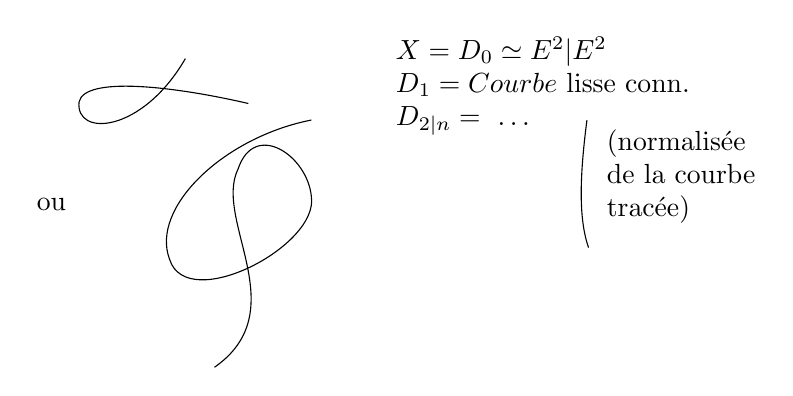
\begin{tikzpicture}[x=1cm,y=1cm]
\draw (1.0,3.5) .. controls (.45,2.55) and (-.40,2.50) .. (-.35,2.95) .. controls (-.28,3.28) and (.85,3.15) .. (1.80,2.93);
\node at (-.70,1.65) {ou};
\draw (2.60,2.72) .. controls (1.48,2.50) and (.55,1.60) .. (.80,.95) .. controls (1.02,.25) and (2.70,1.12) .. (2.60,1.75) .. controls (2.55,2.27) and (1.88,2.72) .. (1.67,2.10) .. controls (1.35,1.45) and (2.40,.30) .. (1.37,-.42);
\node[anchor=north west,align=left] at (3.55,3.90) {$X=D_0\simeq\unsure{\mathbb E^2|E^2}$\\$D_1=\unsure{\text{Courbe}}$ \uline{lisse} conn.\\$D_{\unsure{2|n}}=\varnothing\ \ldots$};
\draw (6.10,2.72) .. controls (6.00,1.95) and (6.00,1.45) .. (6.12,1.10);
\node[anchor=north west,align=left] at (6.23,2.72) {(normalisée\\de la courbe\\tracée)};
\end{tikzpicture}}
qui ne peut être décrit par la donnée d'un diviseur sur $X$, \deleted{lorsqu'on \unsure{en a choisi}}

\deleted{tel diviseur, dans}

L'opération de $\unsure{\mathfrak S_d|G_d}$ sur $\mathbb Z^d$ permet de construire sur $D_d$ un système local
\[
(183)\qquad T_d=D'_d\mathbin\wedge_{(\unsure{\mathfrak S_d|G_d})_{D_d}}(\mathbb Z^d)_{D_d},
\]
\deleted{\unsure{ou}} qui donne naissance à un groupe analytique (et $=$ algébrique) relatif sur $D_d$:
\[
(184)\qquad G_d=T_d\otimes_{\mathbb Z}\mathbb G_{m\,D_d}\simeq\unsure{D'_d|D_d^d}\mathbin\wedge_{(\unsure{\mathfrak S_d|G_d})_{D_d}}\mathbb G_m^d
\]
\deleted{Enfin} et $T_d$ s'interprète en termes de $G_d$ comme le syst. local des $\pi_1$ ou $H_1$ des fibres
\margin{120}
\scanpage{122}
\mspage{60}
On désigne par $T'_d$ l'image inverse de $T_d$ sur $D'_d$, sur lequel $\unsure{\mathfrak S_d|G_d}$ opère donc (c'est un \deleted{rev.} syst. local sur $(D'_d,\unsure{\mathfrak S_d|G_d})\simeq D_d$). Or sur $D'_d$ on a les \inserted{$d$} morphismes
\[
(185)\qquad s_i:D'_d\longrightarrow D_1\qquad(1\leq i\leq d)
\]
permutés par $\unsure{\mathfrak S_d|G_d}$, et d'autre part, si $D_1\longrightarrow D_0$ est une immersion \uline{régulière} \inserted{de codim 1}, on a \deleted{le \inserted{sur $D_1$} \unsure{faisceau}} le faisceau \uline{normal} par l'immersion
\[
(186)\qquad L_1\quad\begin{gathered}\text{faisceau inversible}\\\text{canonique sur }D_1\end{gathered}
\]
et on peut considérer sur $D'_d$ les $d$ faisceaux inv.
\[
(187)\qquad L_{d,i}=s_i^*(L_1)\qquad1\leq i\leq d.
\]
Ils correspondent à des torseurs sous $(\mathbb G_m)_{D_d}$
\[
(188)\qquad\underline L_{d,i}^*=\begin{gathered}\mathbb G_{m\,D_d}\text{-torseur sur }D_d\text{ associé}\\\text{au faisceau inv. }L_{d,i}
\end{gathered}
\]
et on peut considérer
\[
(189)\qquad P'_d=\prod_{1\leq i\leq d}\underline L_{d,i}^*\qquad\text{torseur sous }\mathbb G_m^d
\]
Comme $\unsure{\mathfrak S_d|G_d}$ opérant sur $D'_d$ permute les \inserted{$s_i$ donc les} $\underline L_{d,i}$ entre eux, il opère sur $P_d$, \deleted{qui} \inserted{de} \deleted{devient} façon compatible avec son opération sur
\margin{121}
\scanpage{123}
\[
(190)\qquad G'_d\overset{\mathrm{def}}{=}\mathbb G_{m\,D'_d}\otimes_{\mathbb Z}T'_d\simeq\underbrace{\mathbb G^{d}_{m\,D'_d}}_{\substack{\text{avec opération de}\\\unsure{\mathfrak S_d|G_d}\text{ donnée par}\\\text{permutation des}\\\text{facteurs}}}
\]
et par descente on trouve sur $D_d$ un torseur
\[
(191)\qquad P_d\quad\text{torseur sur }D_d,\text{ de groupe }G_d,
\]
et par suite on a aussi
\[
(192)\qquad T_d\simeq\begin{gathered}\text{\unsure{syst.} local des }H_1\text{ (ou des }\unsure{\pi_1|\pi_0}\text{)}\\\text{des fibres de }P_d
\end{gathered}
\]
On considère le groupoïde fondamental $\Pi P_d$ de $P_d$, et \deleted{le groupoïde} \inserted{(quand} $D_d^*$ est défini comme $D_d\setminus(\text{image des }D_{d',d}\longrightarrow D_d\text{ pour }d'>d,\text{ cf plus bas})$, plus essentiellement pour la suite,
\[
\Pi(\underbrace{P_d\mid D_d^*}_{\overset{\mathrm{def}}{=}\unsure{T_d^*|P_d^*}})=\Pi P_d^*.
\]
On va considérer la variation des objets précédents $T_d,G_d,\inserted{P_d,P_d^*,}T'_d,G'_d,P'_d,\Pi P_d,\Pi\unsure{P_d^*|P''_d}$ \margin{(un couple)} pour $d$ variable. Considérons donc
\deleted{$d\geq d'$}
\[
d\geq d'\geq0
\]
d'où \deleted{\unsure{avec}}
\diagram{\begin{tikzcd}[ampersand replacement=\&, column sep=large,row sep=large]
\&D_{d,d'}\arrow[dl,"\text{rev. ét.}"']\arrow[dr,"\text{imm. loc.}"]\&\\
\unsure{D_d|D_d^*}\&\&D_{d'}
\end{tikzcd}}
\margin{122}
\scanpage{124}
\mspage{61}
Considérons les images inverses de $T_d$ et $T_{d'}$ sur $D_{d,d'}$, qu'on va noter
\deleted{$\unsure{T_d}_{D_{d,d'}}$}
\[
(193)\quad\left\{\begin{aligned}
T(d,d')_d&=(T_d)_{D_{d,d'}}&&\text{syst. local de rang }d\text{ sur }D_{d,d'}\\
T(\unsure{d|d^*},d')_{d'}&=(T_{d'})_{D_{\unsure{d|d^*},d'}}&&\text{syst. local de rang }d'\text{ sur }D_{d,d'}
\end{aligned}\right.
\]
on a alors un hom. canonique surjectif (dit ``tautologique'')
\[
(194)\qquad T(d,d')_d\longrightarrow T(d,d')_{d'}
\]
qui, par image inverse sur $D'_{d,d'}=D'_d\mathbin\times_{D_d}D_{d'}$ (cf diagramme can.

(195)\quad
\diagram{\begin{tikzcd}[ampersand replacement=\&, column sep=large,row sep=large]
\&\mathcal P_{d'}(I_d)_{D'_d}\simeq D'_{d,d'}\arrow[dl]\arrow[dr,"\unsure{\mathfrak S_d|\mathfrak S_{d'}}"]\arrow[rr,dashed]\&\&D'_{d'}\arrow[dd,"\mathfrak S_{d'}"]\\
D'_d\arrow[dr,dash,"\mathfrak S_d"']\&\&D_{d,d'}\arrow[dl]\arrow[dr]\&\\
\&D_d\&\&D_{d'}
\end{tikzcd}}
s'identifie à l'hom. de projection
\[
(196)\qquad\mathbb Z^d\unsure{\text{---}|\longrightarrow}\mathbb Z^{d'}
\]
de $\mathbb Z^d$ sur un produit partiel défini par une partie de cardinal $d'$ de l'ens $I_d$ en exposant : $\mathbb Z^d\simeq\mathbb Z^{I_d}$.
\margin{123}
\scanpage{125}
On déduit de (194) un morphisme correspondant (qui est épi lisse)

(197)\quad
\diagram{\begin{tikzcd}[ampersand replacement=\&, column sep=huge,row sep=large]
G(d,d')_d\arrow[r]\arrow[d,equal,"\mathrm{def}"']\&G(d,d')_{\unsure{d'}}\arrow[d,equal,"\mathrm{def}"]\\
\begin{gathered}G_d\mathbin\times_{D_d}D_{d,d'}\\\simeq T(d,d')_d\otimes_{\mathbb Z}\mathbb G_m\end{gathered}\&\begin{gathered}G_{d'}\mathbin\times_{D_{d'}}D_{d,d'}\\\simeq T(d,d')_{d'}\otimes_{\mathbb Z}\mathbb G_m\end{gathered}
\end{tikzcd}}
et on voit que l'on a un isom. correspondant

(198)\quad
\diagram{\begin{tikzcd}[ampersand replacement=\&, column sep=large,row sep=large]
P(d,d')_{\unsure{d'}}\arrow[r,equal,"\sim"]\arrow[d,equal,"\mathrm{def}"']\&\underbrace{P(d,d')_d}\mathbin\wedge_{G(d,d')_d}G(d,d')_{d'}\arrow[d,equal,"\mathrm{def}"]\\
P_d\mathbin{\unsure{\times|\otimes}}_{D_d}D_{d,d'}\&P_{d'}\mathbin\times_{D_{d'}}D_{d,d'}
\end{tikzcd}}

On a des relations de transitivité
\deleted{Au niveau des groupoïdes fondamentaux, on peut dire que $\Pi P(d,d')_{d'}$}
pour les morphismes précédents,
\deleted{$\unsure{\Pi P(d,d')_d}$}
\unsure{relatifs} à la donnée d'un triple
\[
d\geq d'\geq d''
\]
en se plaçant sur $D(d,d',d'')$, où on a des \deleted{objets} systèmes locaux
\[
(199)\qquad T(d,d',d'')_d,\quad T(d,d',d'')_{d'},\quad T(d,d',d'')_{d''},
\]
des tores correspondants
\[
(200)\qquad G(d,d',d'')_d,\quad G(d,d',d'')_{d'},\quad G(d,d',d'')_{d''}
\]
\margin{124}
\scanpage{126}
\mspage{62}
et des torseurs sous ceux-ci
\[
(201)\qquad P(d,d',d'')_d,\quad P(d,d',d'')_{d'},\quad \unsure{M|P}(d,d',d'')_{d''},
\]
en prenant les images inverses des quantités correspondantes sur $D\deleted{(d)}_{\inserted{d}},D\deleted{(d')}_{\inserted{d'}},D\deleted{(d'')}_{\inserted{d''}}$ par
\diagram{\begin{tikzcd}[ampersand replacement=\&, column sep=large,row sep=large]
\&D_{d,d',d''}\arrow[dl]\arrow[d]\arrow[dr]\&\\
D_d\&D_{d'}\&D_{d''}
\end{tikzcd}}.
Prenant de $=$ les images inverses, par
\diagram{\begin{tikzcd}[ampersand replacement=\&, column sep=large,row sep=large]
\&D_{d,d',d''}\arrow[dl]\arrow[d]\arrow[dr]\&\\
D_{d,d'}\&D_{d',d''}\&D_{d,d''}
\end{tikzcd}}
des morphismes des types (194), (197), (198), on trouve des transitivités

(202)\quad
\diagram{\(\left\{\begin{gathered}\begin{tikzcd}[ampersand replacement=\&, column sep=large,row sep=huge]
T(d,d',d'')_d\arrow[r,no head]\arrow[rr,bend left=18]\&T(d,d',d'')_{d'}\arrow[r]\&T(d,d',d'')_{d''}\\
G(d,d',d'')_d\arrow[r,no head]\arrow[rr,bend left=18]\&G(d,d',d'')_{d'}\arrow[r,no head]\&G(d,d',d'')_{d''}\\
P(d,d',d'')_d\arrow[r,no head]\arrow[rr,bend left=18]\&P(d,d',d'')_{d'}\arrow[r,no head]\&P(d,d',d'')_{d''}
\end{tikzcd}\end{gathered}\right.\)}.

Toutes ces relations sont essentiellement tautologiques. En voici une qui ne l'est plus, et qui fait \unsure{sûrement} appel à \deleted{toute la force de} l'hypothèse ``croisements normaux'' (dans \unsure{tt|tte} sa force\ldots)
\margin{125}
\scanpage{127}
\deleted{On a envie de définir des torseurs}
\[
\deleted{D_{d,d'}^*=D_{d,d'}\mid D_d^*\quad\text{ouvert de }D_{d,d'}}
\]
\deleted{(quand on fait l'hyp.}

On suppose maintenant que la situation envisagée provient d'un diviseur à croisements normaux $D$ sur $X=D_0$, en déployant celui-ci. Alors \inserted{$\forall\,d\in\mathbb N$} la structure \inserted{de} déploiement \unsure{s'induit|induite} sur les $D_d$ (en posant $D_{\deleted{\unsure{d}}i}^{\langle d\rangle}=D_{d+i,d}$ --- je me \unsure{dispenserai|dispense} de développer au long et au large) avec les $=$ propriétés --- elle provient d'un diviseur à croisements normaux \inserted{$\Theta_d$ \deleted{\unsure{(cf)}}} sur $D_d$, dont le complémentaire du support est noté $D_d^*$.

\deleted{On note}
\[
\deleted{(203)\qquad D_{d,d'}^*=D_{d,d'}\mid D_d^*}
\]
\deleted{ouvert de $D_{d,d'}$ (complémentaire d'un diviseur à croisements normaux $\Delta(d,d')$ sur $D_{d,d'}$)}
\deleted{(image inverse de $\unsure{\Theta(d)|D(d)}$)}

\deleted{On \deleted{pose alors} \inserted{veut définir} \deleted{des} morphismes canoniques de groupoïdes}
\[
\deleted{(203)\qquad\boxed{\Pi_1P_d^*\xrightarrow{\gamma_{d,d'}}\Pi_1P_{d'}^*}\qquad\text{pour }d'<d}
\]
\deleted{\uuline{``hom de générisation''}}
\margin{126}
\scanpage{128}
\mspage{63}
Il faut introduire encore les espaces analytiques
de drapeaux $D_{d_0,d_1,\ldots,d_r}$ pour $d_0\geq d_1\geq\cdots\geq d_r\geq0$
leur somme est notée $D_{\Delta_r}$, où $\Delta_r$ désigne
maintenant l'ens. ordonné
\[
\tag{203}\Delta_r=[0,r]\cap\mathbf N
\]
ou simplexe ordonné type de dim $r$. Cette notation
$D_{\Delta_r}$ est compatible avec la notation $D_J$ pour $J$
ens. fini ordonné ayant un plus petit élément.
Alors $D_{\unsure{I_r|\Delta_r}}$ dépend fonctoriellement de façon
contravariante en $\unsure{I_r|\Delta_r}$, pour les applications
croissantes, entre simplexes, donc on a un
espace analytique $1/2$-simplicial, qu'on désigne par
$\mathcal D_*$, donc
\[
\tag{204}
\underset{\inserted{\text{ou }D_{\Delta_r}}}{\mathcal D_r}
=\deleted{\unsure{D_{\Delta_I}|D_{\Delta_r}}}\inserted{D_{\Delta_r}}
=\coprod_{\substack{(d_0,\ldots,d_r)\in\mathbf N^r\\d_0>d_1\cdots>d_r}}
D_{d_0,d_1,\ldots,d_r}.
\]
\deleted{$\unsure{D_{d_0,d_r}|D_{\Delta_r,d_r}}$}
La composante $D_{d_*}=D_{d_0,d_1,\ldots,d_r}$ est
un revêtement étale fini de $D_{d_0}$, s'identifiant
à
\[
\tag{205}
D_{d_*}=D'_{d_0}\wedge_{(\unsure{\mathfrak S_{d_0}|G_{d_0}})_{D_{d_0}}}
\underbrace{\mathcal P_{d_*}\bigl(\deleted{\unsure{[1,d_0]}}I_{d_0}\bigr)}_{
\substack{\text{ens des « drapeaux de}\\
\text{type }d_*\text{ » de l'ens fini}\\I_{d_0}=[1,d_0]\cap\mathbf N}}
\]
on désigne par $D^*_{d_0,d_1,\ldots,d_r}$ l'image inverse
de $D^*_{d_0}$, qui est donc le complémentaire
de l'image inverse $\Delta_{d_0- d_r}$ du diviseur
$\Theta_{d_0}$ sur $D_{d_0}$. On peut bien sûr plus \unsure{simple-|simple}
\margin{127}
\scanpage{129}
ment définir tout de suite
\[
\tag{206}
\left\{\begin{aligned}
\mathcal D_*^*&=\coprod_{d_0\geq d_1\cdots\geq d_r\geq0}D^*_{d_0,d_1,\ldots,d_r}\\
&=\text{image inverse de }D_*^*=\coprod_{d\in\mathbf N}D_d^*\text{ par}\\
&\quad\text{le morphisme }\unsure{0|o}:\mathcal D_*\longrightarrow D_*\\
&\quad\text{défini par les }D_{d_0,\ldots,d_r}\longrightarrow D_{d_0}\\
&\quad\text{i.e. défini par les }\mathcal D_r\longrightarrow D_*
\end{aligned}\right.
\]
\inserted{applications « premier sommet »}
(transposé de
\diagram{\begin{tikzcd}[ampersand replacement=\&, column sep=small,row sep=small]
\&\bullet\,0\arrow[d]\\
\underset{0}{\bullet}\arrow[ur]\&1\arrow[d]\\
\&2\arrow[d,no head]\\
\&\vdots\arrow[d]\\
\&r
\end{tikzcd}}
)

Nous allons définir
\[
\tag{207}
\left\{\begin{aligned}
P_{d_0,d_1,\ldots,d_r}&=\text{image inverse du }\overbrace{P_{d_0}}^{G_{d_0}\text{-torseur}}\text{ sur }D_{d_0}\\
&\qquad\text{par }D_{d_0,\ldots,d_r}\unsure{\text{---}|\longrightarrow}D_{d_0}\\
P^*_{d_0,d_1,\ldots,d_r}&=P_{d_0,\ldots,d_r}\mid D^*_{d_0,\ldots,d_r}
\end{aligned}\right.
\]
\unsure{c'est}\inserted{\unsure{là|sont}} des torseurs sous les Groupes analytiques
(tores)
\[
\tag{208}
\begin{aligned}
G_{d_0,\ldots,d_r}&=\text{image inverse de }G_{d_0}\\
&\quad\text{sur }\unsure{D_{d_0}|d_0}\text{, par }D_{d_0,\ldots,d_r}\unsure{\text{---}|\longrightarrow}D_{d_0}\\
G^*_{d_0,\ldots,d_r}&=G_{d_0,\ldots,d_r}\mid D^*_{d_0,\ldots,d_r}.
\end{aligned}
\]
On a donc un diagramme $2$-cartésien de groupoïdes
\[
(209)
\]
\diagram{\begin{tikzcd}[ampersand replacement=\&, column sep=large,row sep=large]
\bigl(\widetilde\Pi_{d_0- d_r}\overset{\mathrm{déf}}{=}\Pi_1P^*_{d_0,\ldots,d_r}
\arrow[r]\arrow[d]
\&\Pi_1P^*_{d_0}\bigl(\overset{\mathrm{déf}}{=}\widetilde\Pi_{d_0}\bigr)\arrow[d]\\
\Pi_{d_0,\ldots,d_r}=\Pi_1\unsure{D_{d_0,\ldots,d_r}}\arrow[r]
\&\Pi D_{d_0}\bigl(\overset{\mathrm{déf}}{=}\Pi_{d_0}\bigr)
\arrow[ul,phantom,"2\text{-cart.}" description]
\end{tikzcd}}
\margin{128}
\scanpage{130}
\mspage{64}
les flèches verticales sont des morphismes
d'extensions par des noyaux qui sont des $\mathbf Z^{d_0}$
tordus -- en fait par les systèmes locaux
$T_{d_0}$, et son image inverse sur $D^*_{d_0,\ldots,d_r}$ --
on pose donc
\margin{du moins si les $\pi_2$ de $D_{d_0}^{\unsure{\circ|0}}$ et $D_{d_0}^*$ \unsure{etc.} sont nuls...}
\[
\tag{210}
\left\{\begin{aligned}
T_{d_0,\ldots,d_r}&=\text{image inverse de }\overbrace{T_{d_0}}^{\text{syst. loc.}}\text{ (sur }D_{d_0},\\
&\qquad\text{par }D_{d_0,\ldots,d_r}\unsure{\text{---}|\longrightarrow}D_{d_0}\\
\deleted{\unsure{D^*_{d_0,\ldots,d_r}}=}
&\simeq\text{syst. local des }\pi_1\text{ (ou des }H_1\text{)}\\
&\qquad\text{des fibres de }P_{d_0- d_r}/D_{d_0- d_r}\\
T^*_{d_0- d_r}&=T_{d_0- d_r}\mid D^*_{d_0,\ldots,d_r},
\end{aligned}\right.
\]
\inserted{$(\overset{\mathrm{loc}}{\simeq}\mathbf Z^{d_0})$}
de sorte que $\widetilde\Pi_{d_0,\ldots,d_r}$ est une ext. de
$\Pi_{d_0,\ldots,d_r}$ par $T^*_{d_0- d_r}$.
\margin{du moins si $\pi_2(D^*_{d_0,-d_r})=0\ldots$}

On posera bien sûr
\deleted{\[
\unsure{\widetilde\Pi_{*\Delta_r}|\Pi_{\Delta_r}}=\coprod\Pi_{d_0,\ldots,d_r}
\]}
\[
\tag{211}
\left\{\begin{aligned}
\unsure{G_{\Delta_r}}&=
\coprod_{\substack{\deleted{\unsure{d_r\geq\cdots\geq d_0}}\\(d_0,\ldots,d_r)\in\mathbf N^{r+1}\\d_0\geq d_1\cdots\geq d_r}}
\unsure{G_{d_0,-d_r}|B_{d_0,-d_r}}\qquad\text{groupe sur }D_{\Delta_r}\\
P_{\Delta_r}&=\coprod P_{d_0,-d_r}\qquad\text{torseur sous }G_{\Delta_r}\\
T_{\Delta_r}&=\coprod T_{d_0,-d_r}\qquad\text{système local des}\\
&\hspace{4cm}\pi_1\text{, ou }H_1\text{, de}\\
&\hspace{4cm}G_{\Delta_r}\text{ -- }P_{\Delta_r}\text{, --}\\
G^*_{\Delta_r},\ P^*_{\Delta_r},\ T^*_{\Delta_r}&\qquad\unsure{\text{dés}|\text{dire}}\ \text{les restrictions à }D^*_{\Delta_r}.
\end{aligned}\right.
\]
\margin{129}
\scanpage{131}
\[
\tag{212}
\left\{\begin{aligned}
\Pi_{\Delta_r}&=\Pi_1D^*_{\Delta_r}\qquad\text{groupoïde fond.}\\
&\hspace{4cm}\text{de }D^*_{\Delta_r}\\
\widetilde\Pi_{\unsure{\Delta_r}}&=\Pi_1P^*_{\Delta_r}\qquad\text{et de }P^*_{\Delta_r}
\end{aligned}\right.
\]
donc on a
\[
(213)
\]
\diagram{\begin{tikzcd}[ampersand replacement=\&]\widetilde\Pi_{\Delta_r}\arrow[r]\&\Pi_{\Delta_r}\end{tikzcd}}
qui fait de $\widetilde\Pi_{\Delta_r}$ un groupoïde
extension de $\Pi_{\Delta_r}$ par $T_{\Delta_r}$.
Notons « pour mémoire »
\[
\tag{214}
\left\{\begin{aligned}
\Pi_{\Delta_r}&=\coprod_{d_0\geq d_1\geq\cdots\geq d_r}\Pi_{d_0,d_1,\ldots,d_r}\\
\widetilde\Pi_{\Delta_r}&=\coprod_{d_0\geq\cdots\geq d_r}\widetilde\Pi_{d_0,d_1,\ldots,d_r}
\end{aligned}\right.
\]
\margin{\deleted{\unsure{au fait}}}
le système local $T_{\Delta_r}$ sur $\Pi_{\Delta_r}$ \deleted{\unsure{pourra}}
\unsure{s'identifiant|s'identifie} aux systèmes locaux
$T_{d_0\cdots d_r}$ sur les $\Pi_{d_0,\ldots,d_r}$.

Les $\Pi_{\Delta_r}$ n'ont pas de « dépendance
simpliciale » p.r. aux $\Delta_r$, p. ex. on n'a
pas de morphisme naturel entre
$\Pi_{d,d'}=\Pi_1D^*_{d,d'}$, et $\Pi_{d'}=\Pi_1D^*_{d'}$, (\unsure{par|car}
\margin{130}
\scanpage{132}
\mspage{65}
contre il y en a entre $\Pi_{d,d'}$ et $\Pi_d$.
Précisons ce point, en considérant un
morphisme
\[
(215)
\]
\diagram{\begin{tikzcd}[ampersand replacement=\&]\Delta_r\arrow[r,"\alpha"]\&\Delta_{r'}\end{tikzcd}}
\uuline{tel que} $\alpha(0)=0$
alors $D_{\Delta_{r'}}\longrightarrow D_{\Delta_r}$ est un morphisme
étale fini, donc aussi $D^*_{\Delta_{r'}}\unsure{\text{---}|\longrightarrow}D^*_{\Delta_r}$ induit
au dessus de $D^*_{\Delta_r}$, donc on trouve
un diagramme $2$-cartésien (qui \deleted{\unsure{suit|vient}}
\deleted{(209)} \unsure{aussi} se déduit de (209)
\[
(216)
\]
\diagram{\begin{tikzcd}[ampersand replacement=\&, column sep=large,row sep=large]
\widetilde\Pi_{\Delta_{r'}}\arrow[r]\arrow[d]\&\widetilde\Pi_{\Delta_r}\arrow[d]\\
\Pi_{\Delta_{r'}}\arrow[r]\&\Pi_{\Delta_r}\arrow[ul,phantom,"2\text{-cart.}" description]
\end{tikzcd}}
)
\margin{Ceci montre que les $\widetilde\Pi_{\Delta_r}\longrightarrow\Pi_{\Delta_r}$ et $\widetilde\Pi\unsure{\text{---}|\longrightarrow}\Pi$ sont connus \unsure{quand on} connaît les $\widetilde\Pi_d\longrightarrow\Pi_d$, \unsure{des projections locales|des fibrations locales}.}
\margin{\deleted{et les $\unsure{\Pi_d|P_d}$ \unsure{comme}}
\deleted{\diagram{\begin{tikzcd}[ampersand replacement=\&]\unsure{\Pi_d|P_d}\arrow[r]\&\unsure{G_d|\Pi_d}\end{tikzcd}}}
$D_d^*!$ sur $D_{\unsure{\Delta_r|\Delta}}$
\deleted{\diagram{\begin{tikzcd}[ampersand replacement=\&]\unsure{D_d}\arrow[r]\&\unsure{D^*_{\Delta_r}}\end{tikzcd}}}}
où les flèches horizontales induisent sur
les $\pi_1$ des applications injectives à
image d'indice fini (on peut dire que
$\Pi_{\Delta_{r'}}\unsure{\text{---}|\longrightarrow}\Pi_{\Delta_r}$ fait de $\Pi_{\Delta_{r'}}$ un
rev. fini de $\Pi_{\Delta_r}$).

Toutes ces relations sont encore de
nature essentiellement formelle et triviale,
et marcheraient dans un site quelconque,
sans l'hypothèse spécifique des croisements
normaux, et sans que le remplacement des
\margin{131}
\scanpage{133}
$D_{\Delta_r}$ par les $D^*_{\Delta_r}$, pour définir les
$\Pi_{\Delta_r}$ et $\widetilde\Pi_{\Delta_r}$, \inserted{semble y}
jouer\deleted{\unsure{a|ait}} un rôle particulier.
\inserted{et}
Pour \uline{$d_0$ fixé}, les systèmes
\diagram{\begin{tikzcd}[ampersand replacement=\&]
\widetilde\Pi_{d_0d_1-d_r}\arrow[r,no head]\&\Pi_{d_0,-d_r}
\end{tikzcd}}
\unsure{forment|font} un hom de groupoïdes semi-
simpliciaux, mais de nature essentiellement
triviale (il faudrait cepend.t examiner
à l'occasion de plus près cette soi-disant
trivialité -- \unsure{?} elle s'explicite sans peine
en termes de la théorie de Galois
des revêtements de $D^*_{d_0}$ resp. de $P^*_{d_0}$ --).

Nous allons maintenant introduire
un élément de structure tout à fait
non-formel, qui ne peut s'obtenir
qu'avec des hypothèses \unsure{de voisinages}
\unsure{d'intersection normale}, et s'exprimant
par le fait que les $\widetilde\Pi_{\Delta_r}$ (NB et
non les $\Pi_{\Delta_r}$ !) forment un groupoïde
$1/2$ simplicial, pour $\Delta_r$ variable. En d'autres
\margin{132}
\scanpage{134}
\mspage{66}
termes, il faut introduire, \deleted{\unsure{des cas}}
pour un morphisme
\[
(218)
\]
\diagram{\begin{tikzcd}[ampersand replacement=\&]\Delta_r\arrow[r,no head,"\alpha"]\&\Delta_{r'}\end{tikzcd}},
un \uline{morphisme correspondant} de groupoïdes
\[
(219)
\]
\diagram{\fbox{\begin{tikzcd}[ampersand replacement=\&]\widetilde\Pi_{\Delta_{r'}}\arrow[r,"\widetilde\alpha^*"]\&\Pi_{\Delta_r}\end{tikzcd}}}
qu'on appellera l'\uline{hom de générisation}
associé à $\alpha$.
\margin{\figure{\begin{tikzpicture}\draw (0,0)--(0,1);\draw (.05,0)--(.05,1);\end{tikzpicture}}}
Comme $\alpha$ se factorise
canoniquement en un hom surjectif
suivi d'un hom injectif de simplexes,
on est ramené à examiner séparément
les deux cas. Mais si $\alpha$ est surjectif
(« hom de dégénérescence »), \deleted{l'homomorphisme}
\inserted{on a $\alpha(0)=0$}
donc on est dans le cas déjà envisagé --
\deleted{\unsure{correspondant}}\inserted{d'ailleurs} dans ce cas
\diagram{\begin{tikzcd}[ampersand replacement=\&]D^*_{\Delta_{r'}}\arrow[r]\&D^*_{\Delta_r}\end{tikzcd}}
\unsure{se}
décompose en des morphismes
\[
(220)
\]
\diagram{\begin{tikzcd}[ampersand replacement=\&]
D^*_{d'_0,\ldots,d'_{r'}}\arrow[r]\&D^*_{\unsure{d_0|d'_0},\ldots,\unsure{d_r|d'_r}}
\end{tikzcd}},
$(d_0,\ldots,d_r)$ est déduite de $(d'_0,\ldots,\unsure{d'_r|d'_{r'}})$
en \unsure{réécrivant} cette suite, en répétant certains
de ses éléments -- et \deleted{les} alors (220) est
un iso -- donc \uline{si $\alpha$ est un hom}
\margin{On voit que la considération des $\widetilde\Pi_{d_0- d_r}$, $\Pi_{d_0,-d_r}$ pour $d_0,\ldots,d_r$ \unsure{non} \uline{strictement} décroissants, et celle de $\alpha^*$, pour $\alpha$ \unsure{non} \uline{stricts} croissants, \unsure{est de la poudre aux yeux}, \unsure{simplement} !.}
\margin{133}
\scanpage{135}
\uline{de dégénérescence}, \uline{alors} (219) \uline{est \unsure{un|une}}
\deleted{\unsure{équiv.}}\uline{isomorphisme}, de nature ess.t triviale.
On est donc réduit à regarder le
cas d'une application \uline{injective} $\alpha$ (« opération
face »), et le \inserted{seul} cas qui \deleted{\unsure{pose}} pose problème
est bien sûr celui où $\alpha(0)\ne0$. Donc
\[
\tag{221}
\left\{\begin{aligned}
d_*&=\{d_0\unsure{\geq|>}d_1\cdots>d_r\},\quad\text{et si}\\
d'_*&=\{d'_0>d'_1\unsure{\geq|>}\cdots>d'_{r'}\}\text{ est }
\deleted{\unsure{une sous-suite}}\inserted{\text{contenu dans }d_*},\\
&\quad d'_0\ne d_0\text{ i.e. }d'_0<d_0,\quad\text{il faut}
\end{aligned}\right.
\]
définir l'hom
\[
(222)
\]
\diagram{\begin{tikzcd}[ampersand replacement=\&]
\Pi_1P^*_{d_0\deleted{\unsure{\geq}}d_1,\ldots,d_r}\arrow[r]\&
\Pi_1P^*_{d'_0,\ldots,d'_r}
\end{tikzcd}}
\margin{Attention, on a subrepticement changé de notations, en intervertissant $d_*$ et $d'_*$ !}
\margin{on se réduit au cas de $d_0,d_1,\ldots,d_r$ strict.t décroissants -- auquel on parvient aussitôt. En fait, on est ramené au cas où $\unsure{r'=r-1}$, et où il s'agit de l'opération « face de codim $1$ » pour laquelle $\alpha(0)\ne0$, donc correspondant :
\diagram{\begin{tikzcd}[ampersand replacement=\&]D_{d_0,d_1,\ldots,d_r}\arrow[r]\&D_{d_1,\ldots,d_r}\end{tikzcd}}}
Notons que l'on a
\[
(223)
\]
\diagram{\begin{tikzcd}[ampersand replacement=\&]
D^{\deleted{*}}_{d_0,\ldots,d_r}\arrow[r]\&D_{d'_0,\ldots,d'_{r'}}
\end{tikzcd}}
(mais \uline{non} un morphisme entre les
espaces avec $*$ !), qui est une immersion \inserted{locale}
d'espaces analytiques lisses, de codim
$d_0-d'_0$, \deleted{qui}\inserted{\unsure{ainsi|et}} s'insère dans le diagramme
\margin{134}
\scanpage{136}
\mspage{67}
\[
(224)
\]
\diagram{\begin{tikzcd}[ampersand replacement=\&]
D_{d_0,\ldots,d_r}\arrow[r]\arrow[d]\&D_{d'_0,\ldots,d'_{r'}}\arrow[d]\\
D_{d_0,d'_0}\arrow[r]\&D_{\unsure{d'_0}}^{\deleted{\unsure{*}}}
\end{tikzcd}}
où les flèches verticales sont étales,
et la $2^{\mathrm{ième}}$ flèche horizontale est une
immersion locale de codim \deleted{$d_0-d'_0$. \unsure{On a}}
\[
\tag{225}\unsure{d|\delta}=d_0-d'_0
\]
[Dans le \unsure{typique} (auquel on se réduit)
où $d'_* = \{\uline{d_1}>\cdots>d_r\}$, le diagramme
(224) est cartésien -- \deleted{\unsure{comme on voit}}\inserted{plus génér.t}, il
\unsure{reste} \deleted{\unsure{tjs}} cartésien, \inserted{si $d'_0=d_1$}, et c'est trivial.]
\margin{\uline{NB} Dans le cas général, on a :
\diagram{\begin{tikzcd}[ampersand replacement=\&, column sep=small]
D_{d_*}\arrow[r,"{\text{fini étale}}"']\arrow[dd,dotted]\&D_{\unsure{\widetilde d_*}}\arrow[r]\arrow[d]\&D_{d'_*}\arrow[d]\\
\&D_{d_0,d'_0}\arrow[dl,dotted]\arrow[r]\&D_{d'_0}\\
D_{d_0}\&\&
\arrow[ul,phantom,from=2-3,to=1-2,"{\text{cart.}}" description]
\end{tikzcd}}}
Considérons le morphisme induit
\[
(225)
\]
\diagram{\begin{tikzcd}[ampersand replacement=\&]D^*_{d_*}\arrow[r]\&D_{d'_*}\end{tikzcd}}
(Attention, on a mis un $*$ en exposant
à $D_{d_*}$ seulement, non à $D_{d'_*}$ !).

Nous munissons $D_{d'_*}$ du diviseur
$\Theta_{d'_*}$ image inverse de $\Theta_{d_0}$ sur $D_{d_0}$.
On désigne par $\Theta_{d'_*}^{(p)}$ le « squelette
de dim $p$ » de $\Theta_{d'_*}^{p}$, et \deleted{\unsure{p}} on pose
\margin{135}
\scanpage{137}
\[
\tag{226}
\Theta_{d'_*}^{\unsure{d}*}\overset{\mathrm{def}}=
\Theta_{d'_*}^{\unsure{d}}\setminus\Theta_{d'_*}^{\unsure{d+1|d1}}
\]
squelette \unsure{purifié|ponctué}
de codim. $d$ de
$\Theta_{d'_*}$ dans $D_{d'_*}$.

Ceci posé, on voit que $225$ \uline{induit}
un \deleted{morphisme} \uline{isomorphisme local}
\uline{de} $D_{d_*}$ \uline{sur} \deleted{$\unsure{D_{d'_*}|\Theta_{d'_*}}$} $\Theta_{d'_*}^{d*}$. Plus
précisément, \deleted{$\Theta_{d'_*}^{d*}$ s'identifie à
$\unsure{D_{d_0,d'_0,\ldots,d'_r}}\quad D_{\unsure{\widetilde d_*}}$, où}
\[
(227)
\]
\diagram{\begin{tikzcd}[ampersand replacement=\&]
\Theta_{d'_*}^{(d)}\&D_{\widetilde d'_*}\arrow[l,"\sim"']
\end{tikzcd}}
où \deleted{\unsure{$d$}}
\[
\widetilde d'_*=(d_0,d'_0,\ldots,d'_r)
\]
et cet isom. induit un isom.
\[
(228)
\]
\diagram{\begin{tikzcd}[ampersand replacement=\&]
D_{\widetilde d'_*}^{*}\arrow[r,"\sim"]\&\Theta_{d'_*}^{(d)*},
\end{tikzcd}}
d'autre part (223) $D_{d_*}\unsure{\longrightarrow|\text{---}}D_{d'_*}$ se
factorise en
\[
(229)
\]
\diagram{\begin{tikzcd}[ampersand replacement=\&]
D_{d_*}\arrow[r,no head]\&D_{\widetilde d'_*}\arrow[r]\arrow[d,no head,"\sim" description]\&D_{d'_*}\\
\&\Theta_{d'_*}^{(d)\unsure{*}}\&
\end{tikzcd}}
donc c'est un morphisme étale fini,
suivi \deleted{d'un}\inserted{\unsure{du|est}} morphisme d'inclusion de
$\Theta_{d'_*}^{(d)}$ dans $D_{d'_*}$. De plus, comme $D_{d_*}^{*}$ est
\margin{136}
